In this chapter, we take another look at a number of components in thermodynamic systems, using entropy to compare their actual performance to their real performance.  After looking specifically at compressors and turbines, we will be able to revisit the Rankine and Refrigeration cycles, as well as explore the Brayton cycle, which is used in jet engines and gas generators.

%====================================================================
\section{Mollier ($h$-$s$) Diagram}
%====================================================================
The primary tool we will use to investigate the efficiency of components is the Mollier, or $h$-$s$ diagram.  In this case, the entalpy is plotted on the $y$-axis, and the entropy on the $s$ axis.  The $h$-$s$ diagram for water is shown in Figure \ref{fig:hs_water}.

\begin{figure}[H]
  \centering
  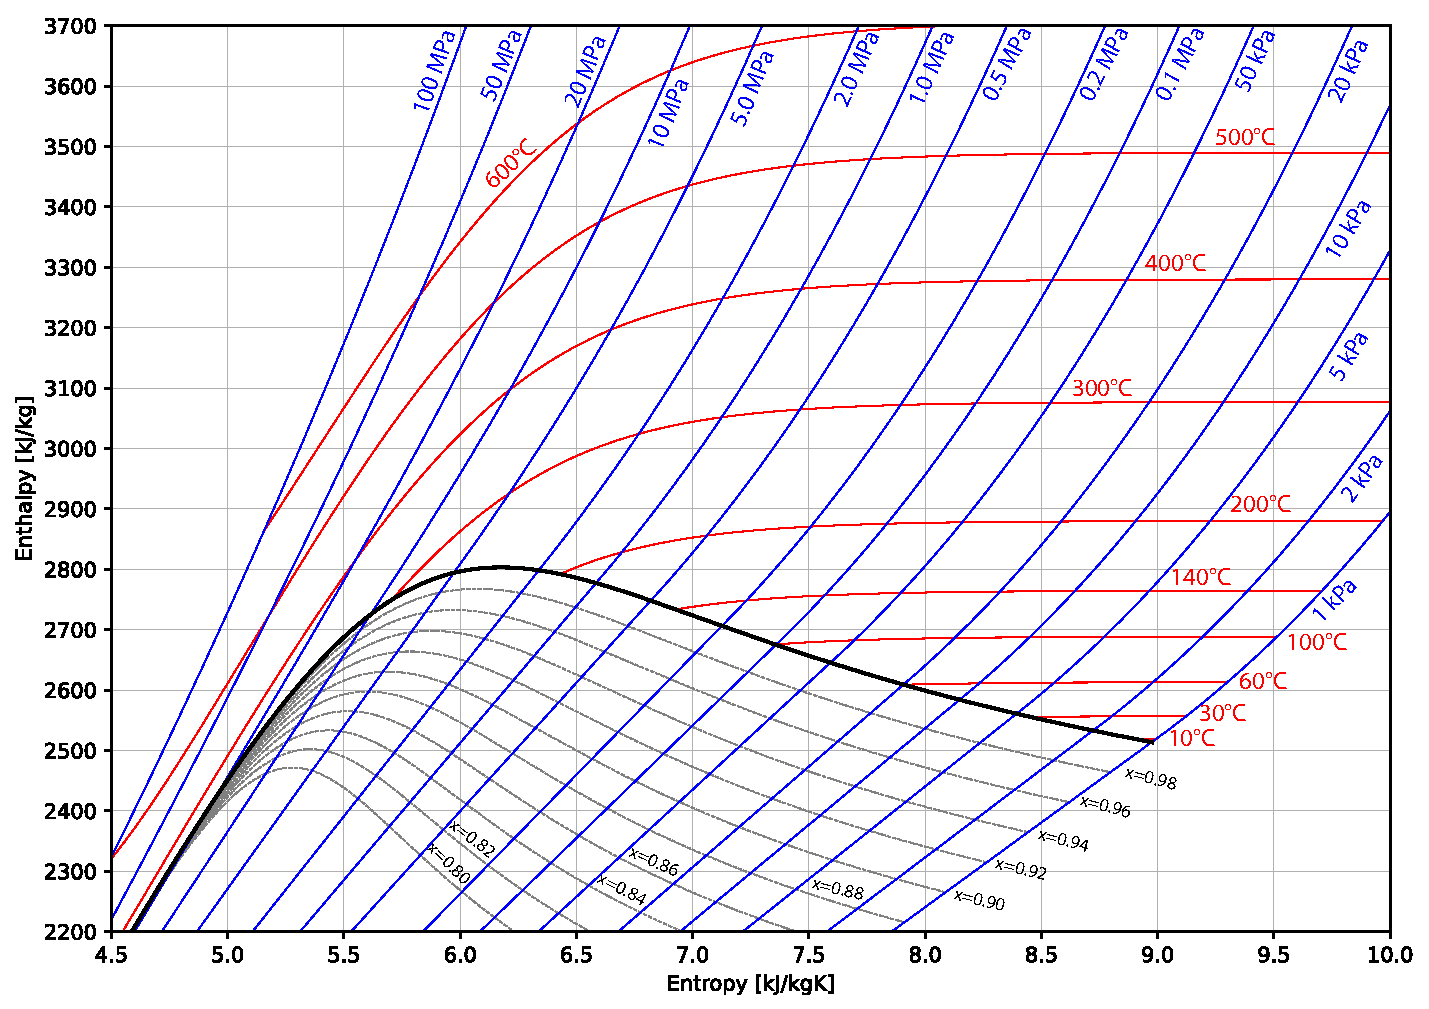
\includegraphics[width=.7\linewidth]{h-s_water}
  \caption{The Mollier, or $h$-$s$ diagram, for water}
  \label{fig:hs_water}
\end{figure}

Notice the focus on superheated steam.  While some of the vapor curve is visible, the vast majority is not shown on the diagram.  Typically, the $h$-$s$ diagram is used for processes which are primarily vapor.  For instance, we will plot a turbine on the $h$-$s$ diagram in Section \ref{sec:turbine_eff}, and a compressor in Section \ref{sec:compressor_eff}.

In some circumstances, an entire cycle can be plotted on the $h$-$s$ diagram.  This is the case for the Brayton cycle, which is used in gas generators and turbojets.  We will analyze the Brayton cycle in Section \ref{sec:Brayton}.

%====================================================================
\section{Isentropic Efficiency}
%====================================================================

One of the important applications of isentropic processes is in defining the ideal performance of various adiabatic components. These include turbines, compressors, pumps, and diffusers and nozzles in aircraft jet engines. Before, we have made the statement that steam turbines are designed to be adiabatic, and that any heat loss from the turbine will result in a reduction in output power. Now, however, we can make the statement that the ideal turbine is isentropic. This enables us to evaluate the {\bf isentropic efficiency} of these components.

\subsection{Isentropic Efficiency of Turbines} \label{sec:turbine_eff}
%--------------------------------------------------------------------
One important characteristic of the $h$-$s$ diagram is that the ideal turbine can be plotted as a vertical line.  An actual turbine will always have an increase of entropy, shown on the $h$-$s$ diagram as a deviation to the right. This is shown in Figure \ref{fig:turbine_eff}.
\begin{figure}[H]
  \centering
  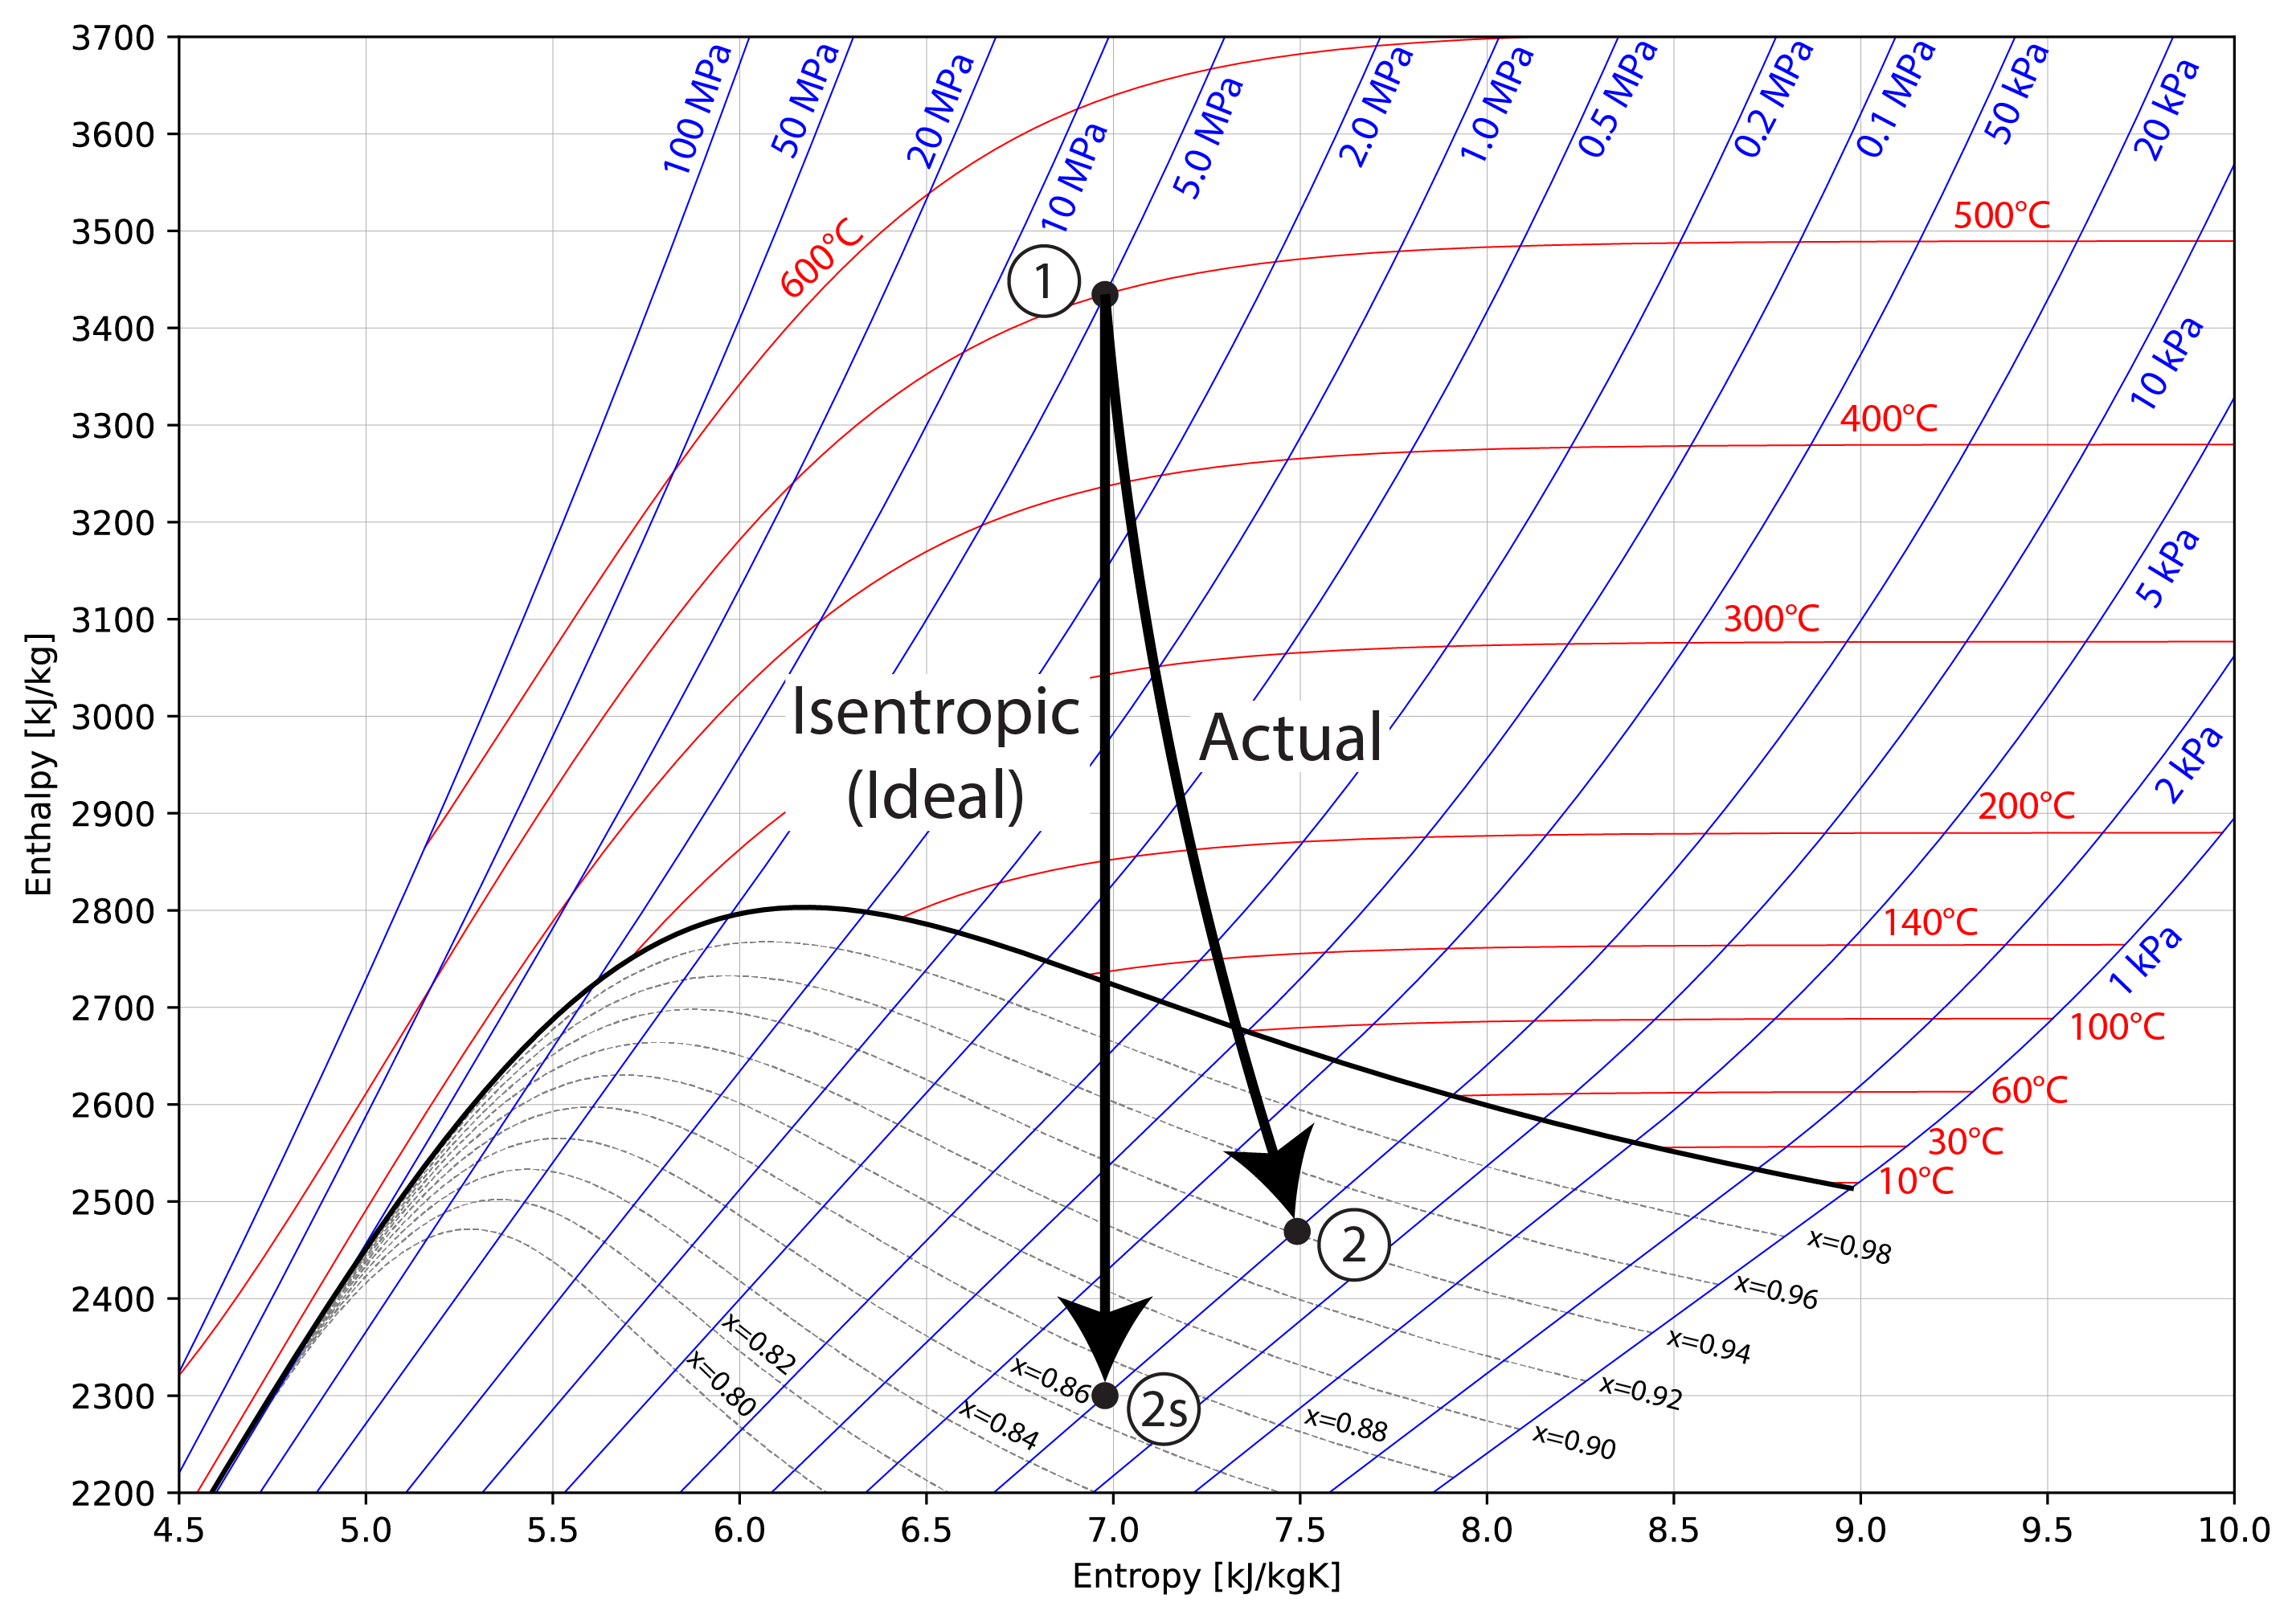
\includegraphics[width=.75\linewidth]{turbinehs}
  \caption{An isentropic turbine process (1-2s) shown next to an actual turbine process (1-2).  Note that the pressure is the same between states 2 and 2s, but the enthalpy changes significantly.}
  \label{fig:turbine_eff}
\end{figure}
The common links between the two processes are the initial state and final pressure.  An increase of entropy with this constraint will always cause a decrease in the amount of work extracted (shown as the vertical distance on the $h$-$s$ diagram).  This leads to the definition of isentropic efficiency for a turbine:
\begin{equation} \label{eq:turbine_eff}
  \eta_T = \frac{\rm actual\ work}{\rm isentropic\ work} = \frac{w_a}{w_s} = \frac{h_1 - h_{2}}{h_1 - h_{2s}}
\end{equation}

The isentropic efficiency is used in Example \ref{ex:isentropicEffTurbine} as a link between the ideal and actual performance of a turbine.

% vvvvvvvvvvvvvvvvvvvvvvvvvvvvvvvvvvvvvvvvvvvvvvvvvvvvvvvvvvvvvvvvvvvv
\begin{example}[label=ex:isentropicEffTurbine]{Steam Turbine Isentropic Efficiency}
  Consider an adiabatic steam turbine having an isentropic efficiency of $\eta_T$ = 80\%, with 2 kg/s of steam coming into the inlet at 1 MPa and 500°C and exiting the turbine at 10 kPa.

  \begin{enumerate}[a)]
  \item Using steam tables, determine the enthalpy and entropy values at state (1) and state (2s) assuming that the turbine is isentropic.
  \item Determine the actual enthalpy and entropy values as well as the temperature at state (2). 
  \item Plot the actual and isentropic turbine processes on the $h$-$s$ diagram, then draw the specific work for each process.
  \item Determine the actual power output of the turbine (kW). 
  \end{enumerate}

  \subsubsection*{Enthalpy and Entropy - States 1 and 2s}
  Since we have two properties for state 1, we can use the steam tables to determine the enthalpy and entropy:

  \begin{align*}
    h_1 &= 3479 \frac{\rm kJ}{\rm kg} & s_1 &= 7.764 \frac{\rm kJ}{\rm kg\,K}
  \end{align*}

  In order to find state 2s, we use the entropy of state 1 (as the process 1-2s is isentropic) and the pressure of state 2, and again go to the steam tables.

  \begin{align*}
    h_{2s} &= 2461 \frac{\rm kJ}{\rm kg} & s_{2s} &= 7.764 \frac{\rm kJ}{\rm kg\,K}
  \end{align*}

  \subsubsection*{Enthalpy, Entropy, and Temperature - State 2a}

  In order to find the properties of state 2a, we need to use the isentropic efficiency:
  \begin{equation*}
    \eta_T = \frac{h_1 - h_2}{h_1 - h_{2s}} \qquad \rightarrow \qquad h_2 = h_1 - \eta_T \left( h_1 - h_{2s} \right)
  \end{equation*}

  Plugging in our values gives:
  \begin{equation*}
    h_2 = 3479 \frac{\rm kJ}{\rm kg} - 0.8 \left( 3479 \frac{\rm kJ}{\rm kg} - 2461 \frac{\rm kJ}{\rm kg} h_{2s} \right) = \redbox{ 2665 \frac{\rm kJ}{\rm kg}}
  \end{equation*}

  This gives us enough information (pressure and enthalpy) to go to the steam tables:

  \begin{align*}
    s_{2s} &= 7.764 \frac{\rm kJ}{\rm kg\,K} & T_{2} &= 88°C
  \end{align*}


  \subsubsection*{$h$-$s$ Diagram}
  \begin{center}
    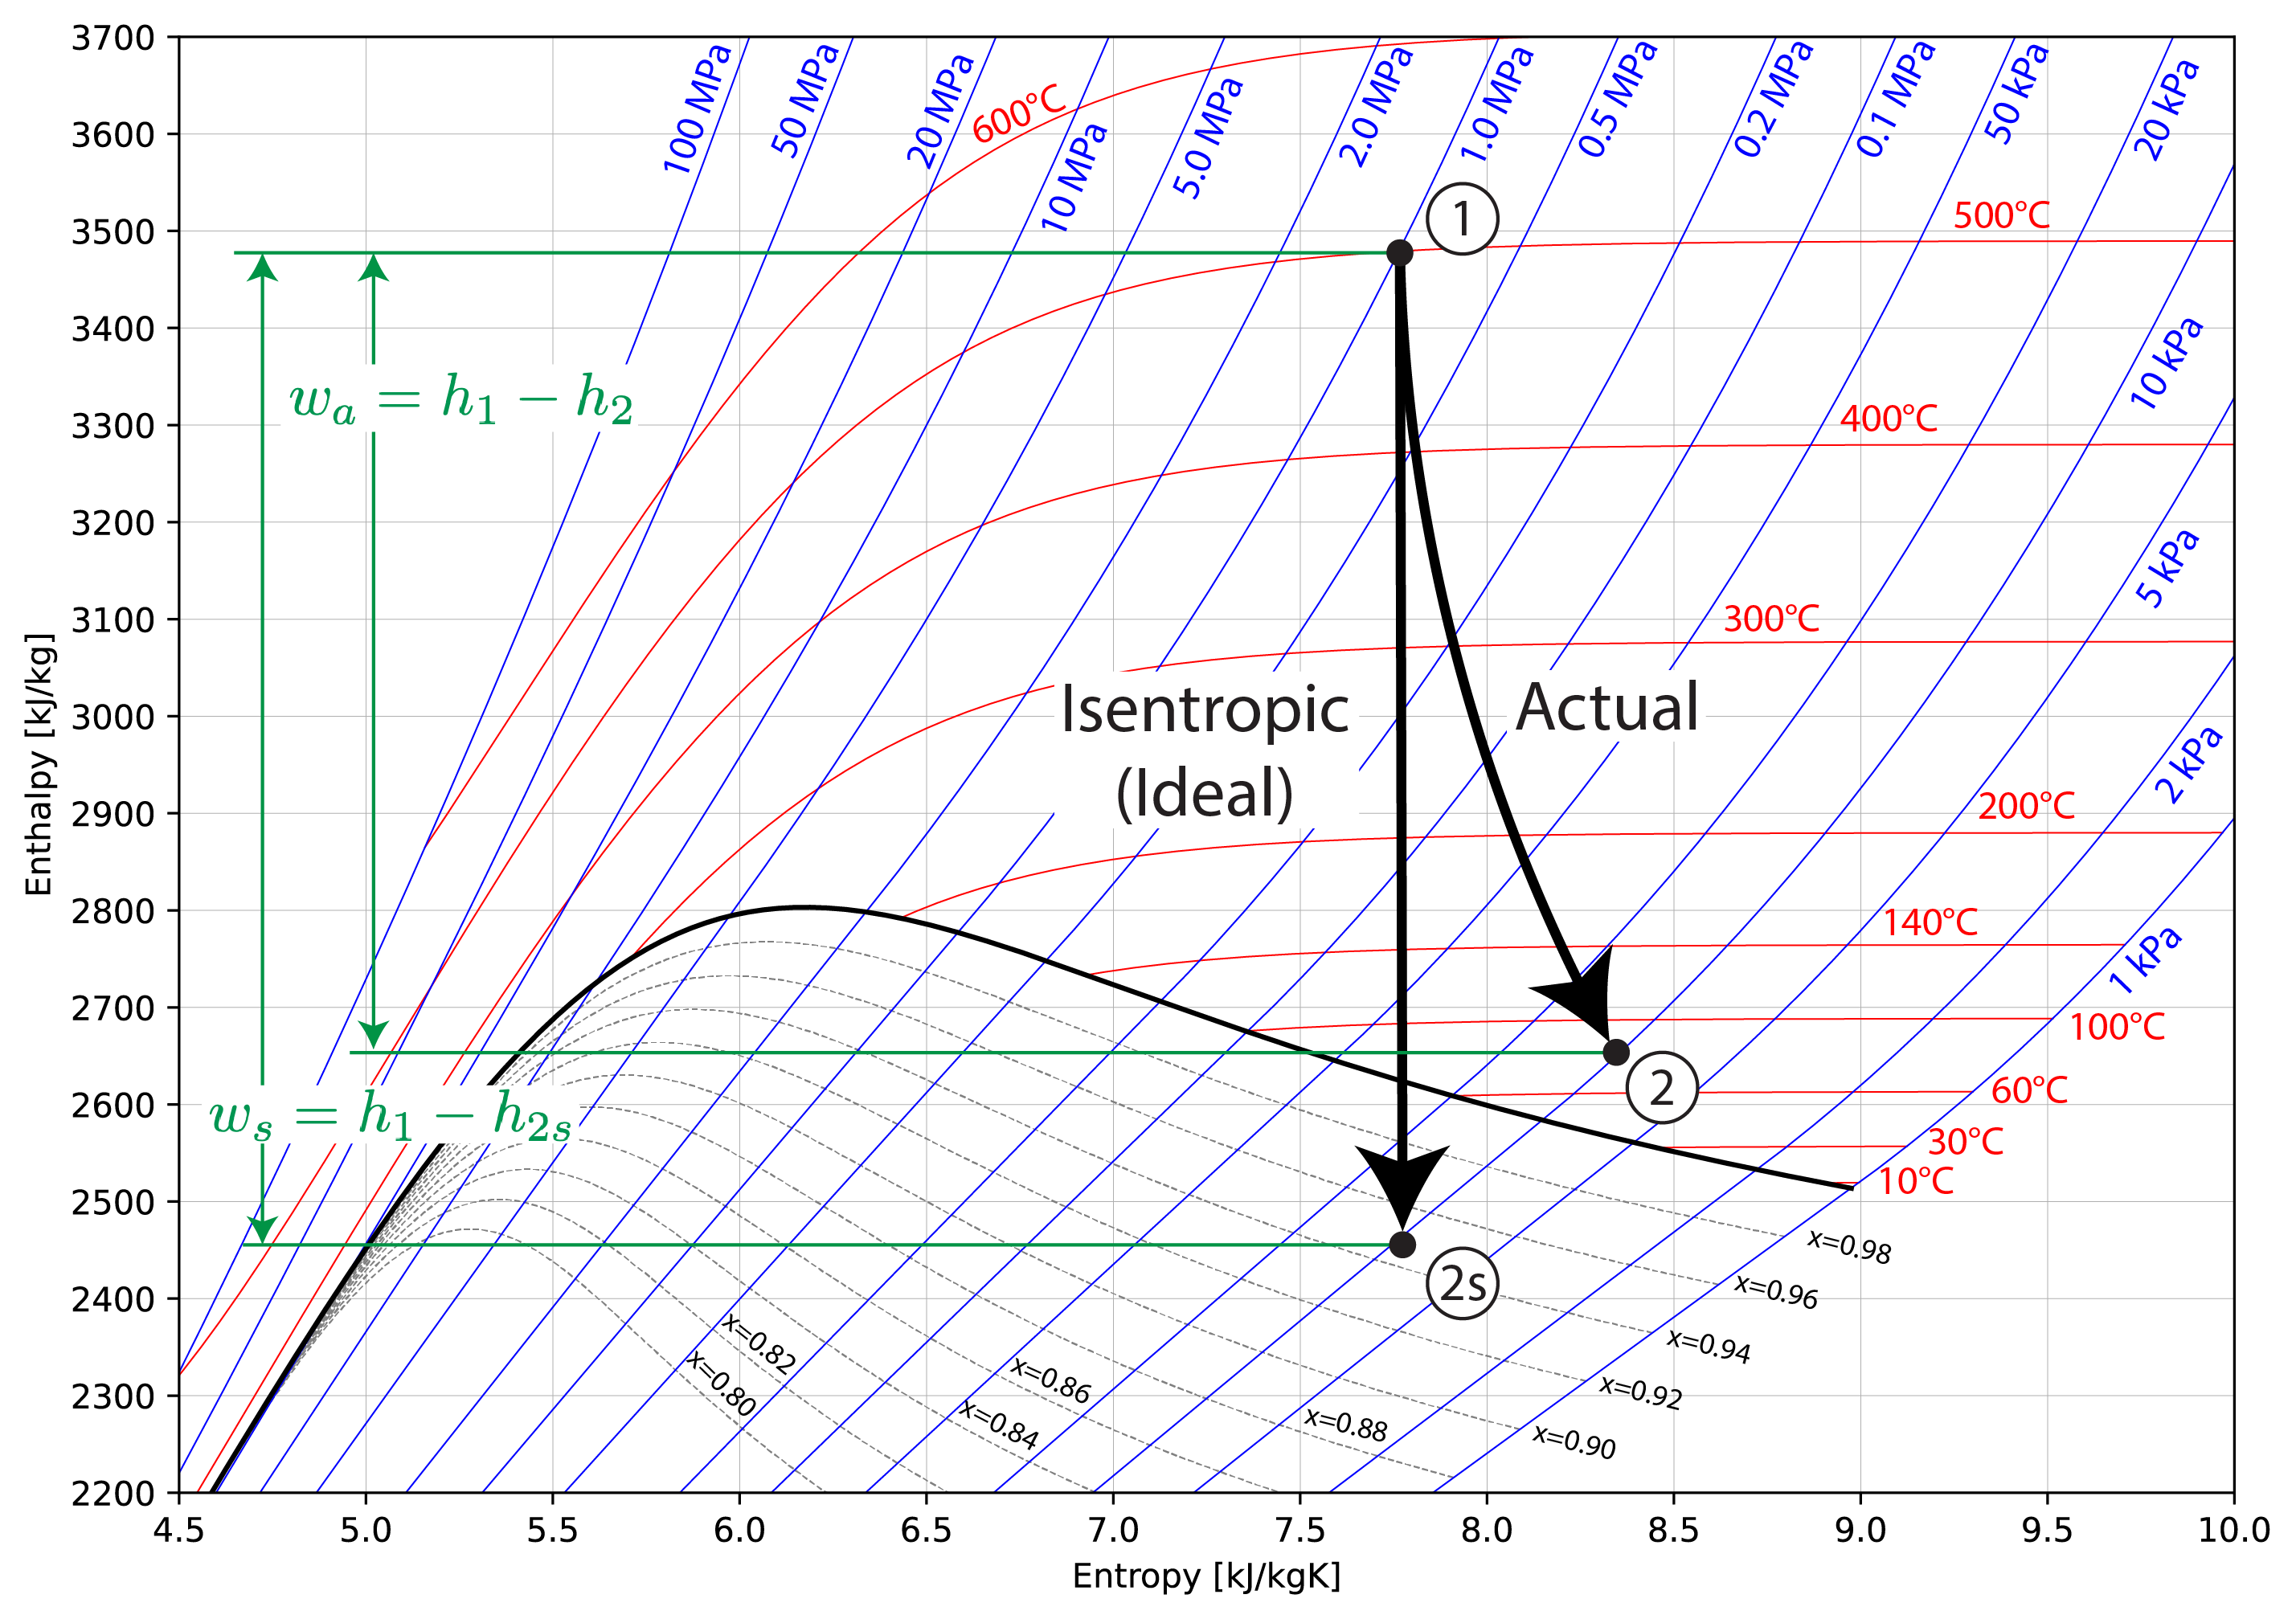
\includegraphics[width=0.8\linewidth]{turbIsentropicEffExample}
  \end{center}
  
  \subsubsection*{Actual Turbine Power}
  The turbine power can be calculated through the simple equation $\dot{W} = \dot{m} w$:
  \begin{equation*}
    \dot{W} = \left(2 \frac{\rm kg}{\rm s}\right) \left(3479 \frac{\rm kJ}{\rm kg} - 2665 \frac{\rm kJ}{\rm kg}\right) = \redbox{1628 \rm kW}
  \end{equation*}
  
\end{example}
% vvvvvvvvvvvvvvvvvvvvvvvvvvvvvvvvvvvvvvvvvvvvvvvvvvvvvvvvvvvvvvvvvvvv

\subsection{Isentropic Efficiency of Compressors} \label{sec:compressor_eff}

As with ideal turbines, ideal compressors are a vertical line on the $h$-$s$ diagram.  Real systems add entropy, which means that the actual process will again veer to the right.  This is shown in Figure \ref{fig:compressor_eff}.

\begin{figure}[H]
  \centering
  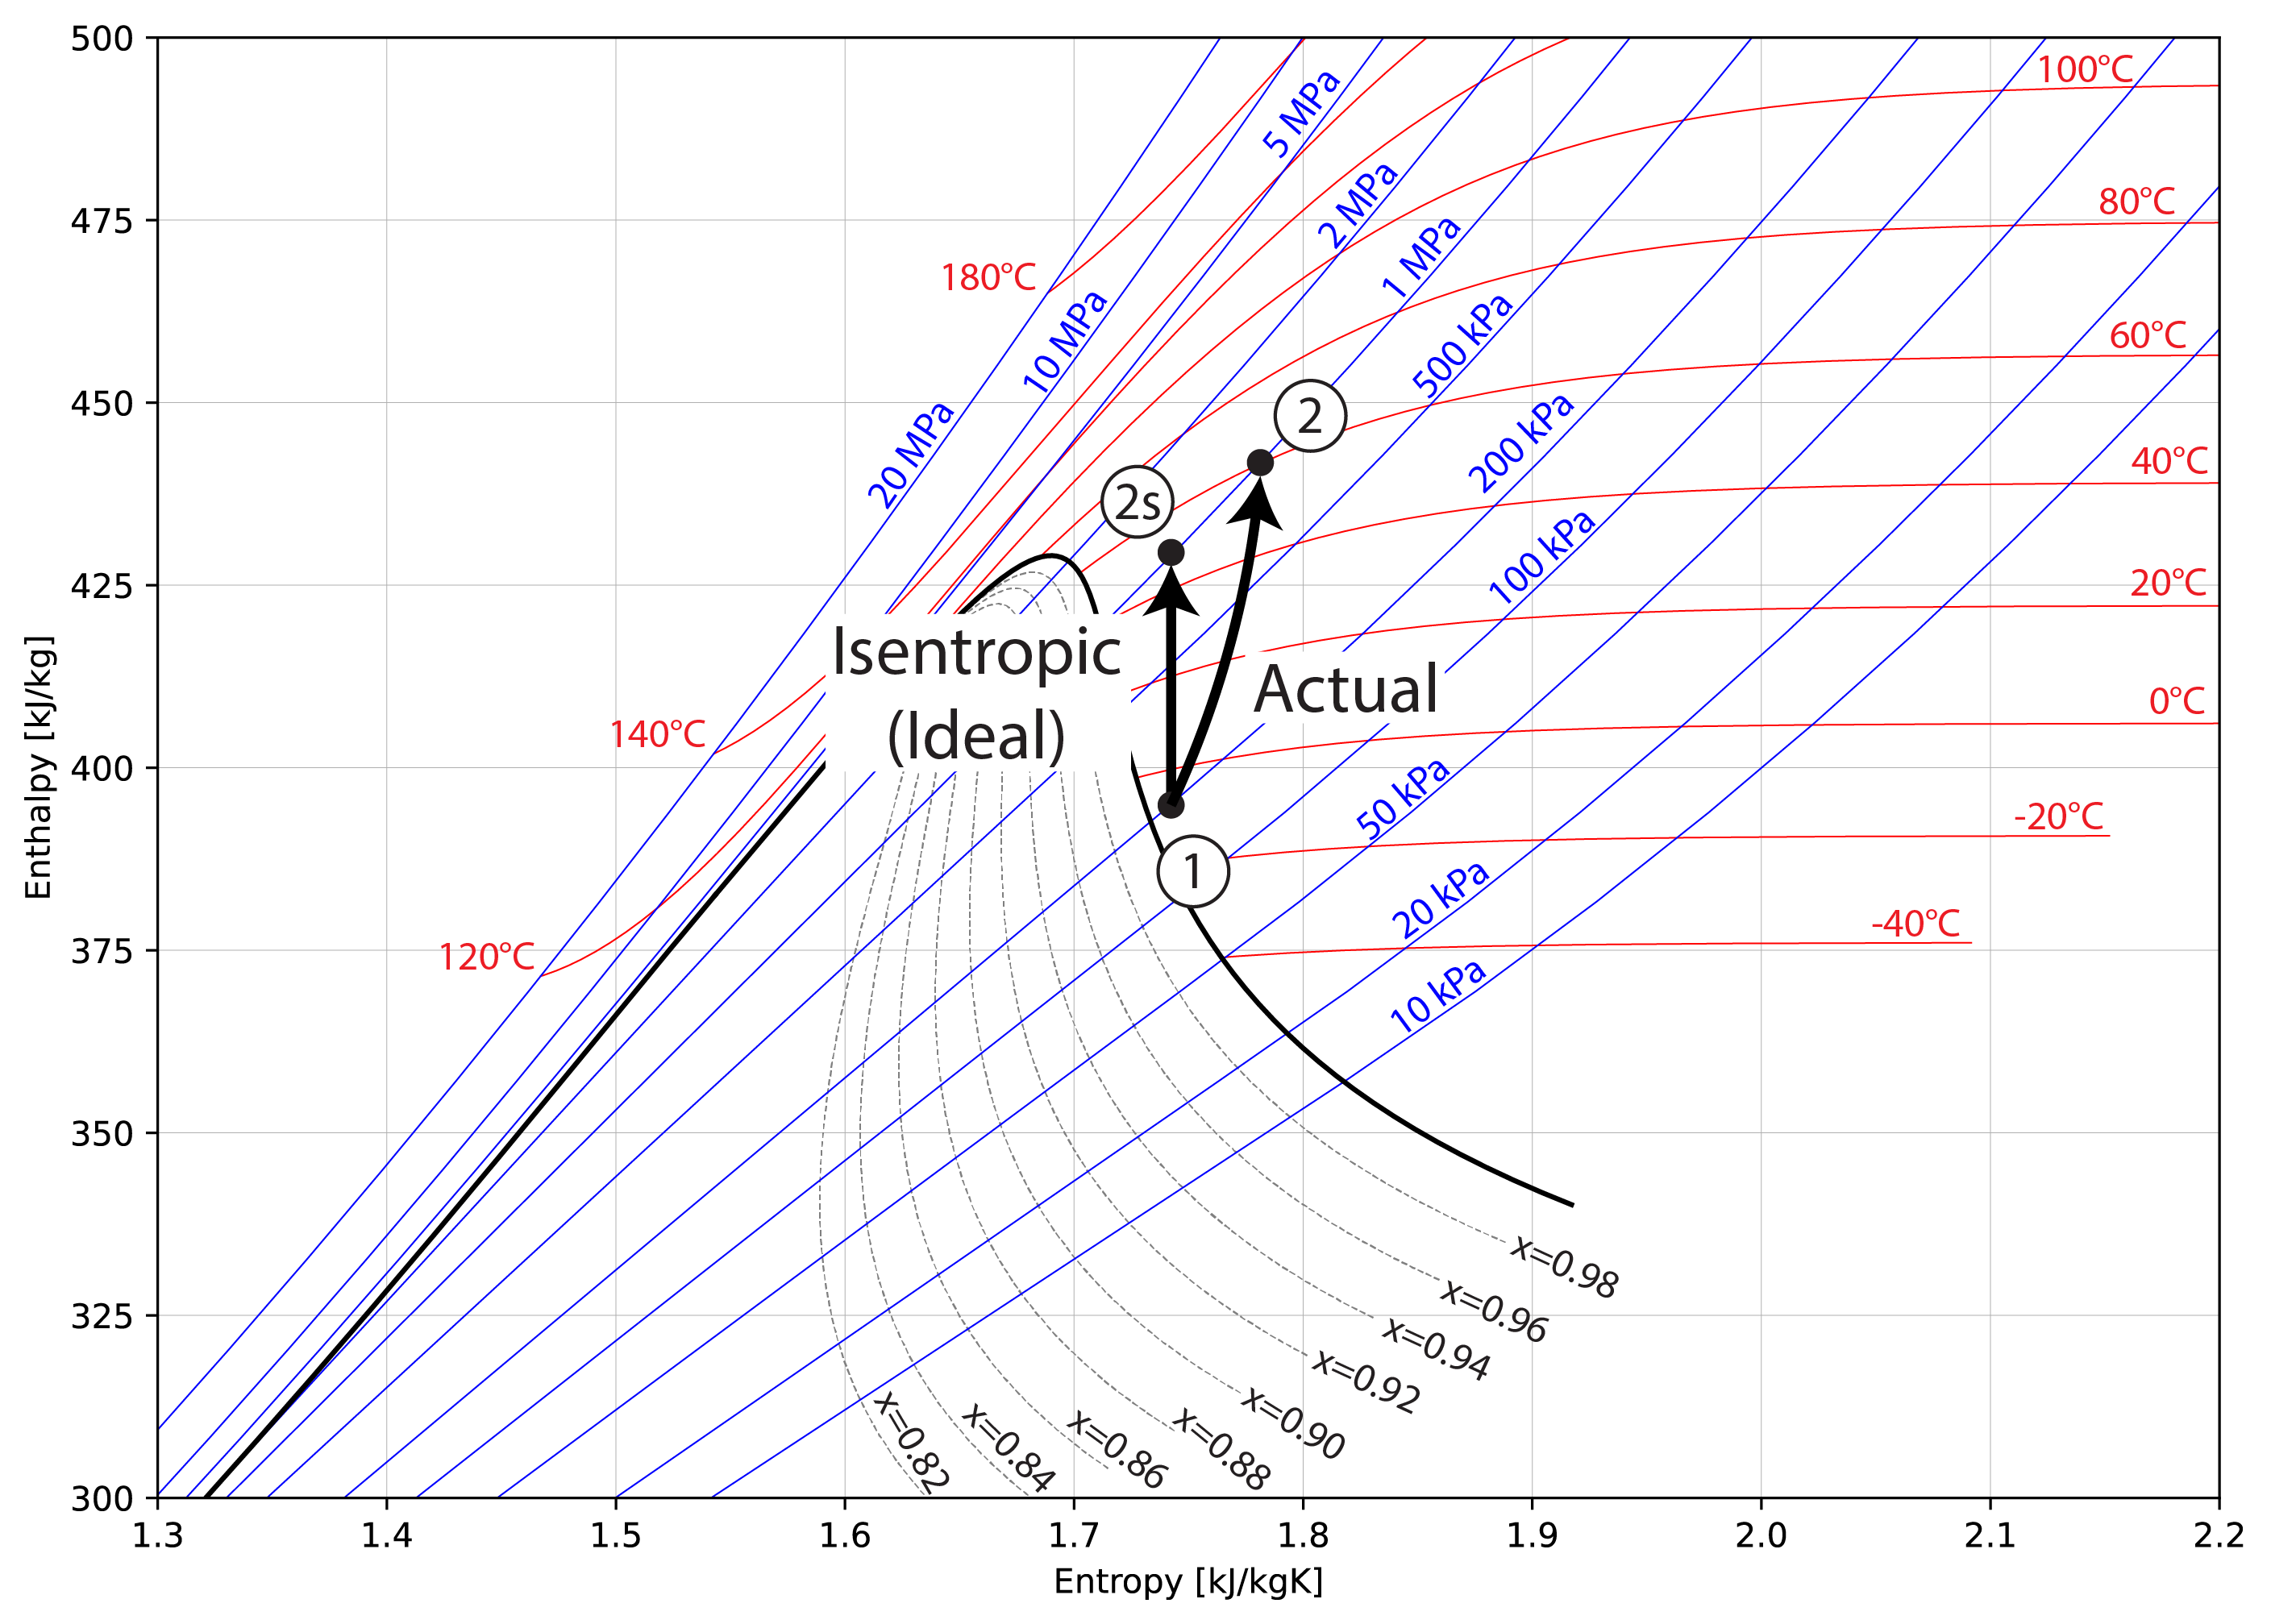
\includegraphics[width=.75\linewidth]{compressorhs}
  \caption{An isentropic compressor process (1-2s) shown next to an actual turbine process (1-2).}
  \label{fig:compressor_eff}
\end{figure}

As with the turbine, both the ideal and actual processes modeling the compressor will start and end at the same pressure.  The increase of entropy in the actual compressor causes an increase in the final enthalpy, which means that the actual compressor requires more work to operate than an ideal compressor.  We therefore define the isentropic efficiency as the inverse of Equation \ref{eq:turbine_eff}:

\begin{equation}\label{eq:comp_eff}
  \eta_C = \frac{\rm isentropic\ work}{\rm actual\ work} = \frac{w_s}{w_a} = \frac{h_{2s} - h_{1}}{h_{2} - h_{1}}
\end{equation}

The isentropic efficiency of a compressor is calculated in Example \ref{ex:isentropicEffCompressor}.

\begin{example}[label=ex:isentropicEffCompressor]{Compressor Isentropic Efficiency}
  Consider an adiabatic compressor that has an inflow of R134a at 100 kPa and -20°C and an outflow at 1 MPa and 60°C.

  \begin{enumerate}[a)]
  \item Plot the actual and isentropic compression processes on the $h$-$s$ diagram, then draw the specific work for each process.
  \item Using R134a refrigerant tables, determine the enthalpy and entropy values at each state (1, 2s, 2).
  \item Calculate the specific work required to drive the compressor.
  \item Determine the isentropic efficiency of the compressor.
  \end{enumerate}
  \subsubsection*{$h$-$s$ Diagram}
  Because both states are known for the actual process, it is trivial to draw on the $h$-$s$ diagram.  In order to draw the ideal process, we simple draw a line straight up from state 1, and continue until we hit the outflow pressure of 1 MPa.

  \begin{center}
    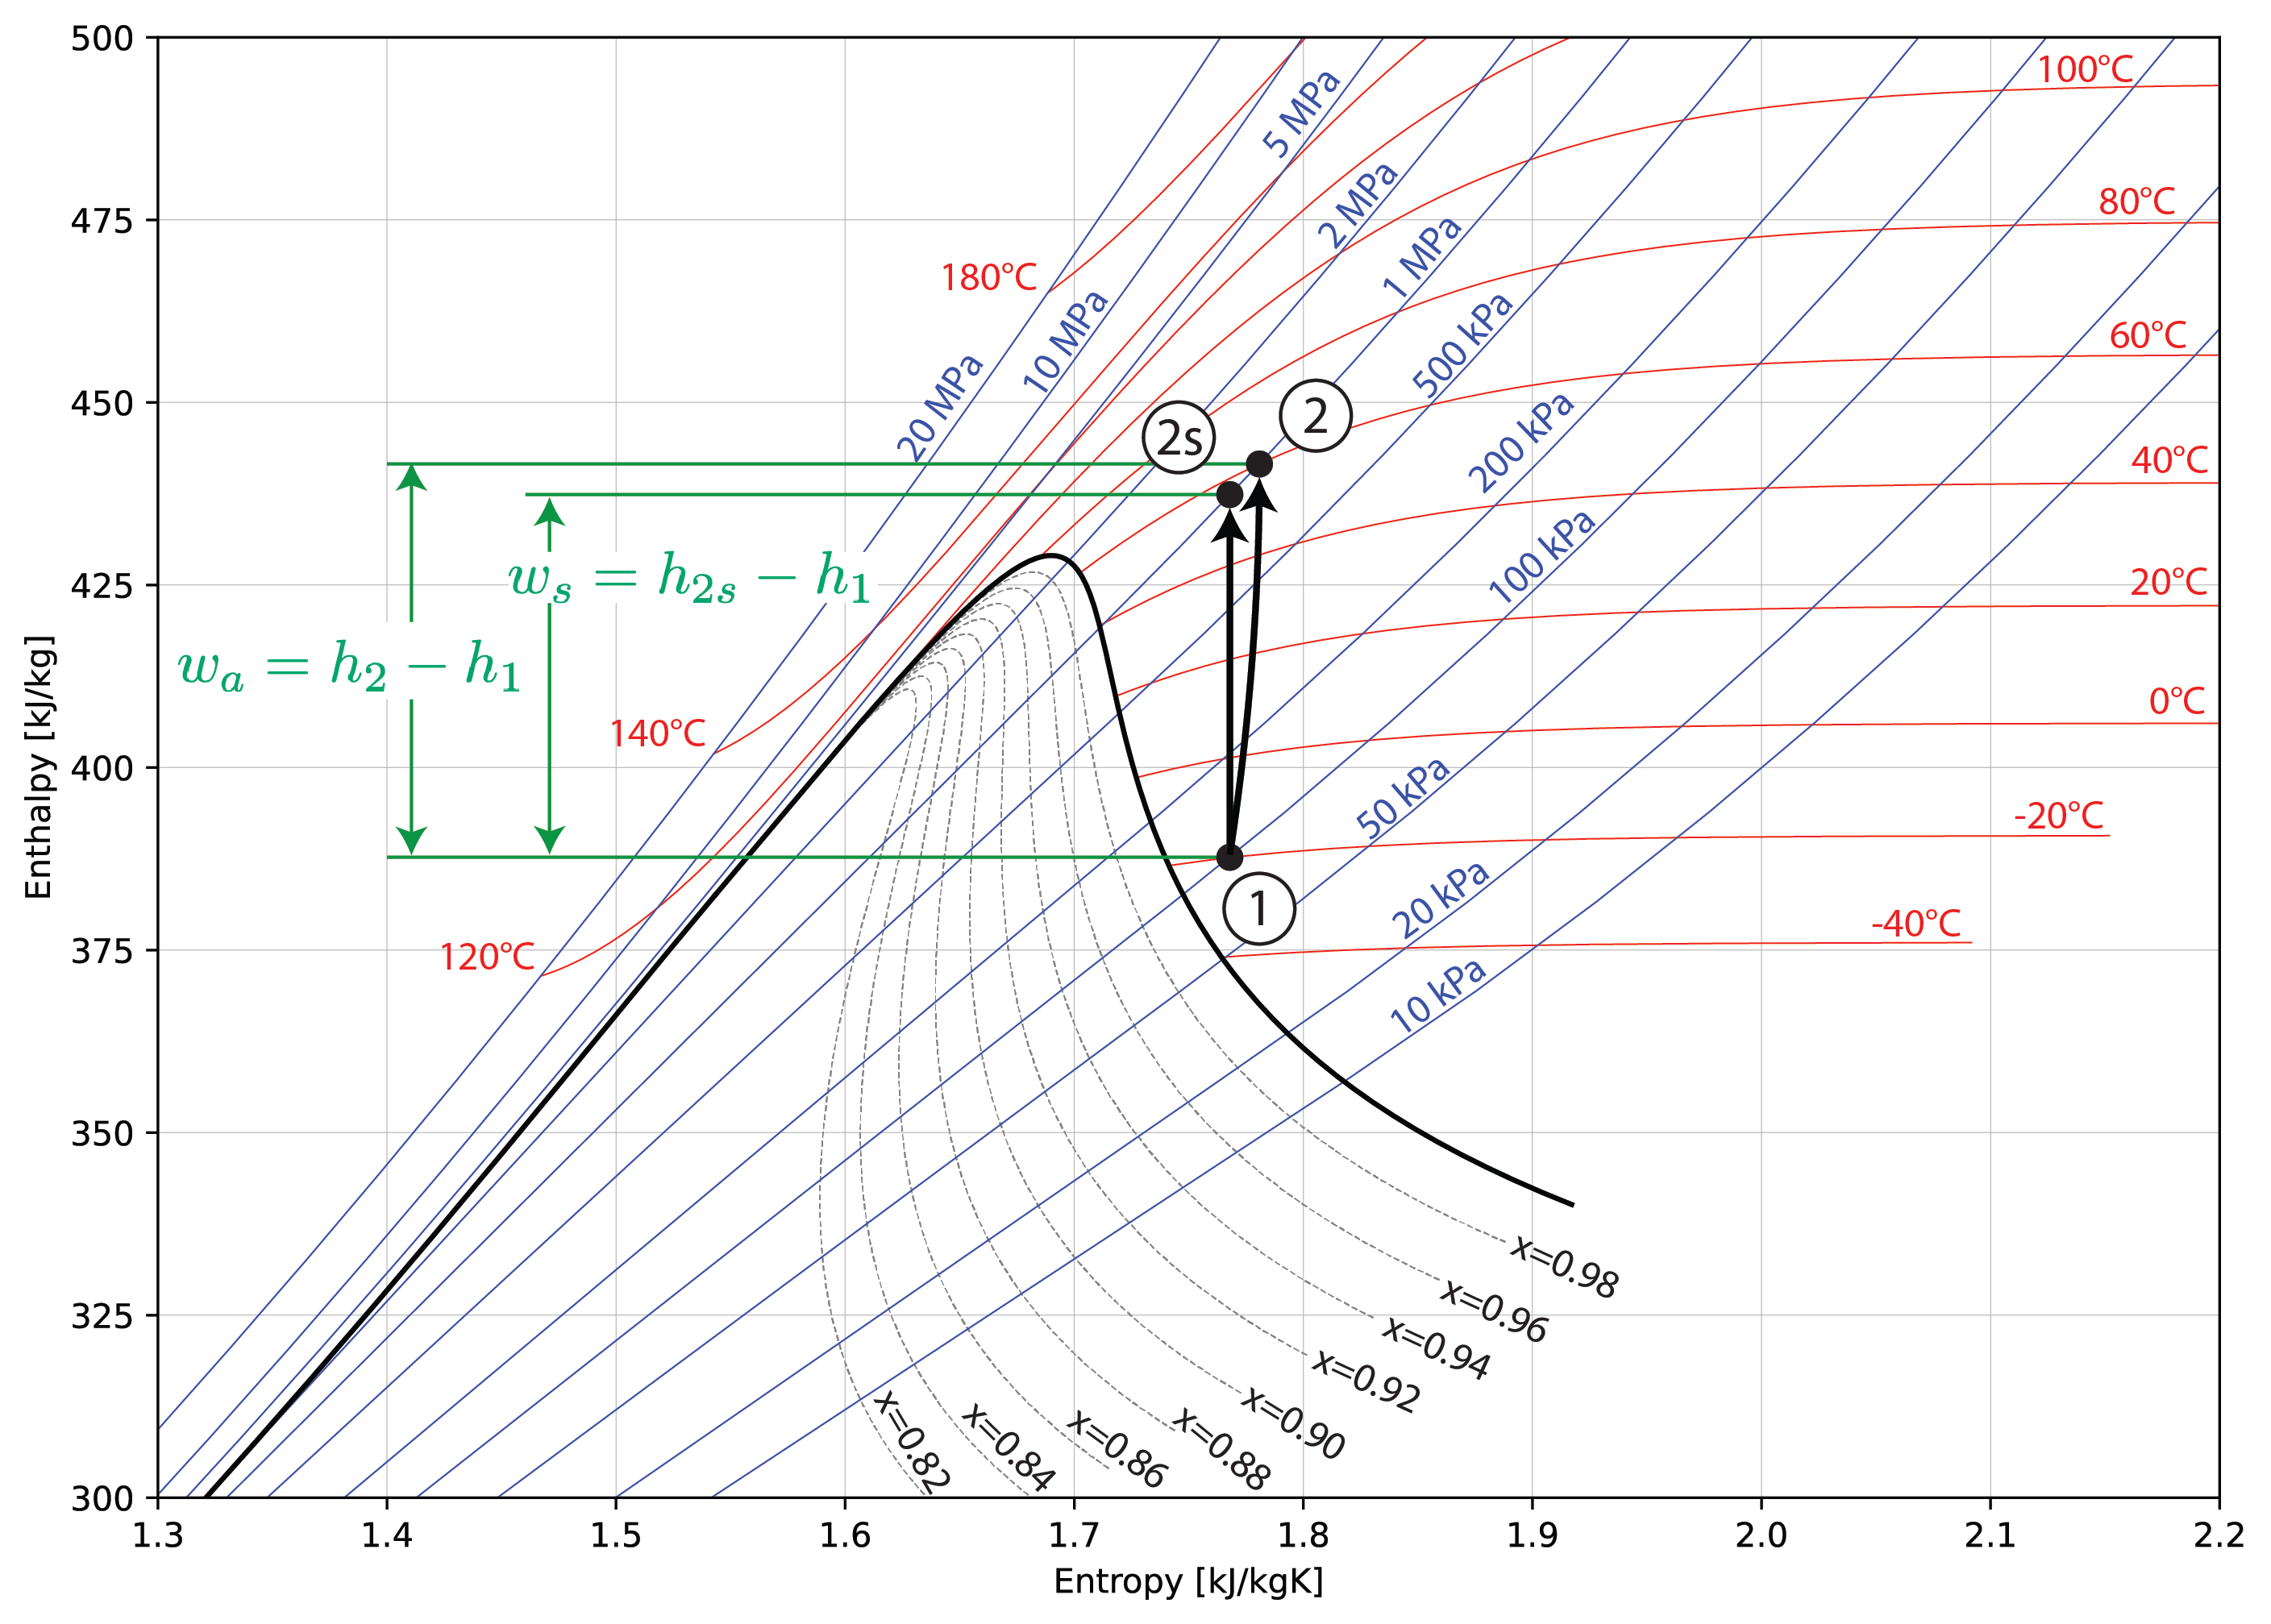
\includegraphics[width=0.75\linewidth]{compIsentropicEffExample}
  \end{center}

  \subsubsection*{Table of Properties}
  The table below lists the pressure, temperature, enthalpy, and entropy for each state.  Properties in black are directly given by the problem statement, properties in blue are inferred based on knowledge of the processes involved, and properties in red are calculated through CoolProp or the R134a tables.
  \begin{table}[H]
    \centering
    \def\arraystretch{1.5}
    %\caption{Tabular Representation of Energy Equation for Stirling Cycle}
    %\label{tab:ch3_stirling}
    \begin{tabular}{r|ccc}
      & State 1 & State 2s & State 2  \\ \hline
      Pressure    & 100 kPa & {\color{Blue} 1 MPa} & 1 MPa  \\
      Temperature & -20°C   & {\color{Red} 56°C}  &   60°C   \\
      Enthalpy    & $\color{Red} 387.6\ \frac{\rm kJ}{\rm kg}$ & $\color{Red} 437.3\ \frac{\rm kJ}{\rm kg}$ & $\color{Red} 441.5\ \frac{\rm kJ}{\rm kg}$ \\
      Entropy     & $\color{Red} 1.768\ \frac{\rm kJ}{\rm kg\,K}$  & $\color{Blue} 1.768\ \frac{\rm kJ}{\rm kg\,K}$  & $\color{Red} 1.781\ \frac{\rm kJ}{\rm kg\,K}$ 
    \end{tabular}
    \def\arraystretch{1.0}
  \end{table}
  \subsubsection*{Specific Work and Isentropic Efficiency}
  Both specific works can be computed as the difference of enthalpies, due to the adiabatic assumption for compressors.
  \begin{align*}
    w_a &= h_2 - h_1 = 53.9 \frac{\rm kJ}{\rm kg} & w_s &= h_{2s} - h_1 = 49.6 \frac{\rm kJ}{\rm kg}
  \end{align*}

  With these in hand, we can use the definition of isentropic efficiency for a compressor:
  \begin{equation*}
    \eta_C = \frac{w_s}{w_a} = \redbox{0.92}
  \end{equation*}
  The isentropic efficiency of this compressor is 92\%.
\end{example}


%====================================================================
\section{The Brayton Cycle} \label{sec:Brayton}
%====================================================================

The Brayton cycle is very similar to the Diesel cycle.  Both are composed of isentropic compression, followed by combustion at constant pressure, followed by isentropic expansion.  Both cycles are plotted on $p$-$v$ and $h$-$s$ diagrams in Figure \ref{fig:BraytonDieselComp}.

\begin{figure}[H]
\centering
\begin{subfigure}{.5\textwidth}
  \centering
  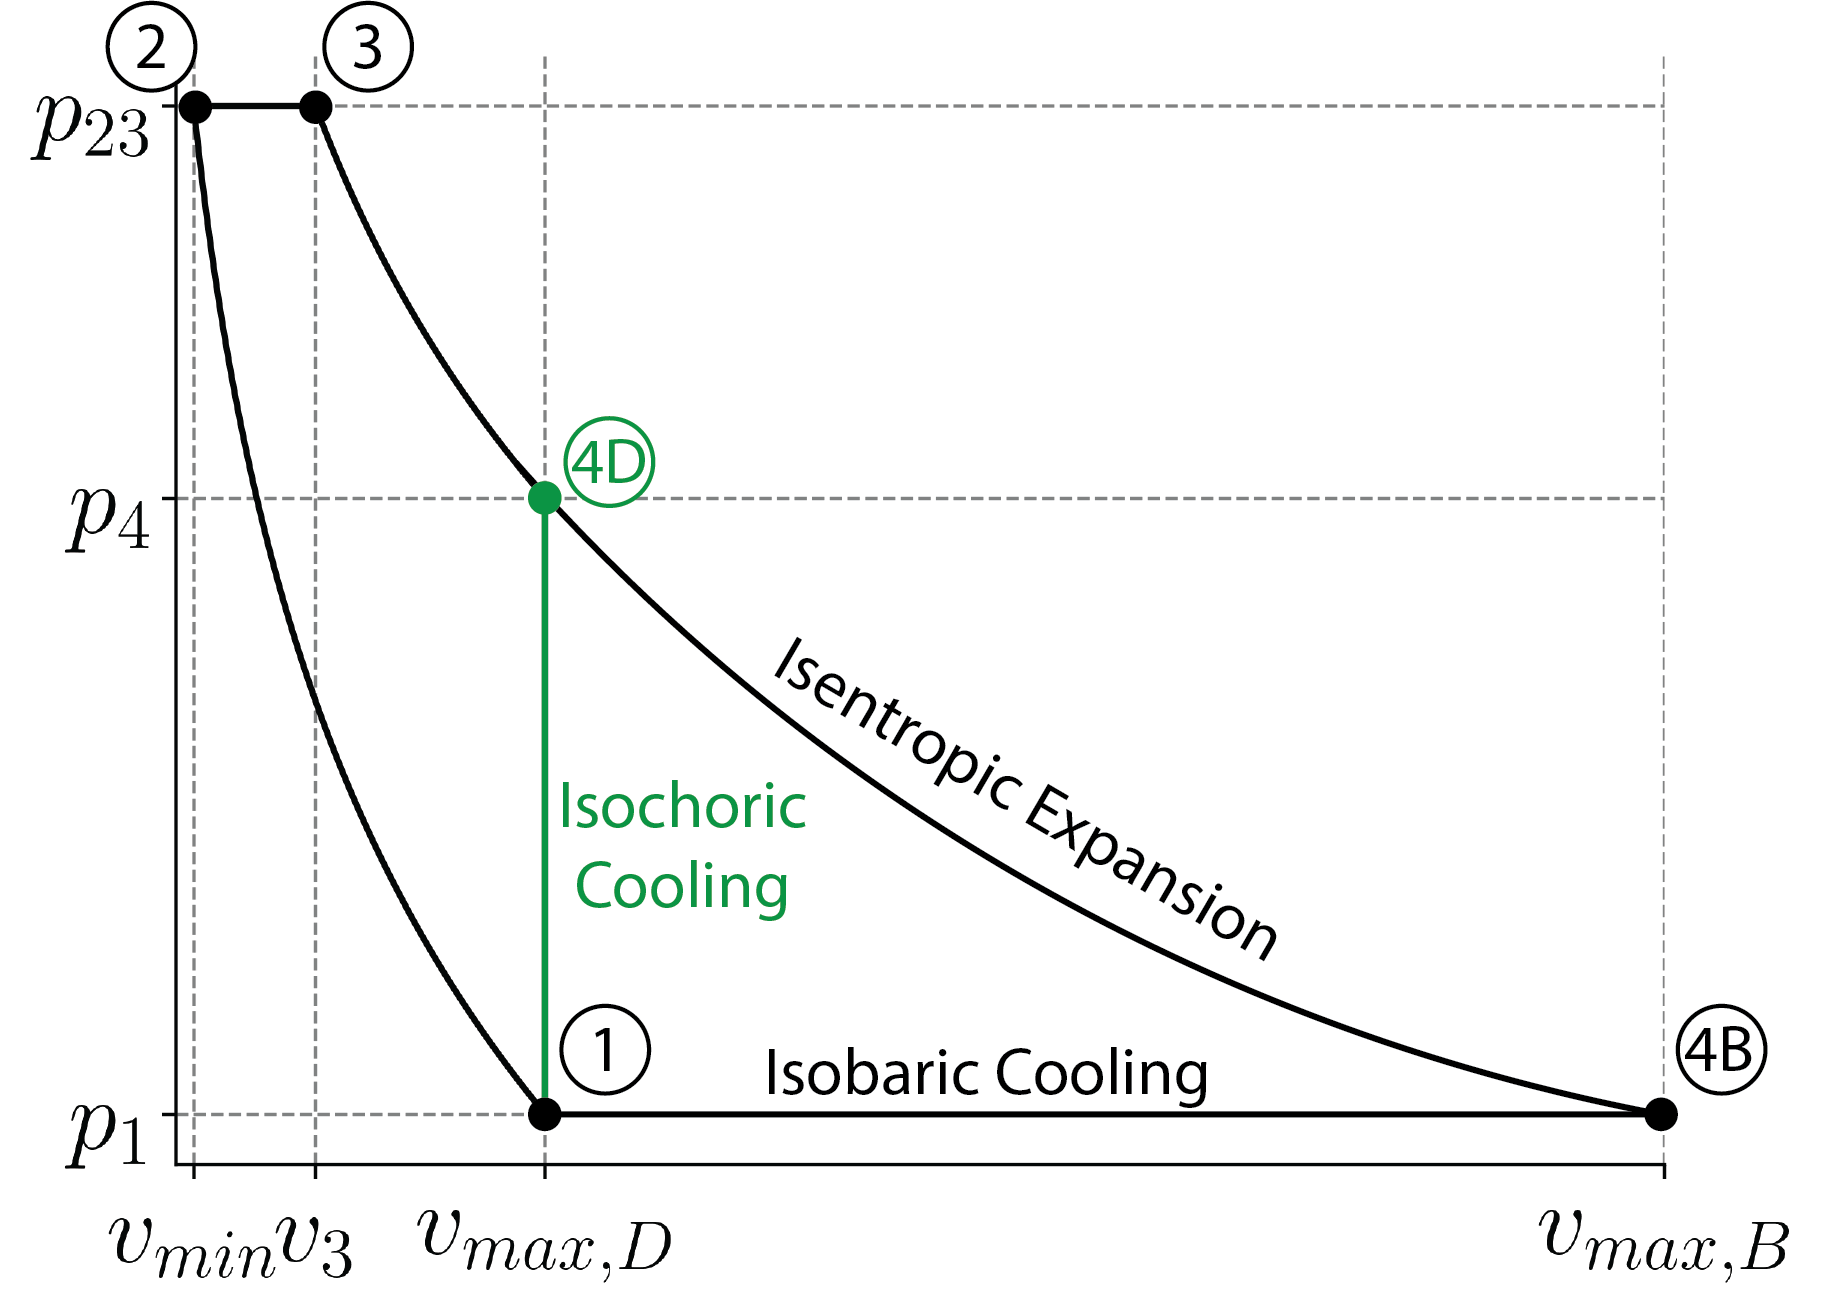
\includegraphics[width=.95\linewidth]{BraytonDieselpv}
  %\caption{Photograph of the GE T700 engine.}
  %\label{fig:t700_baseline}
\end{subfigure}%
\begin{subfigure}{.5\textwidth}
  \centering
  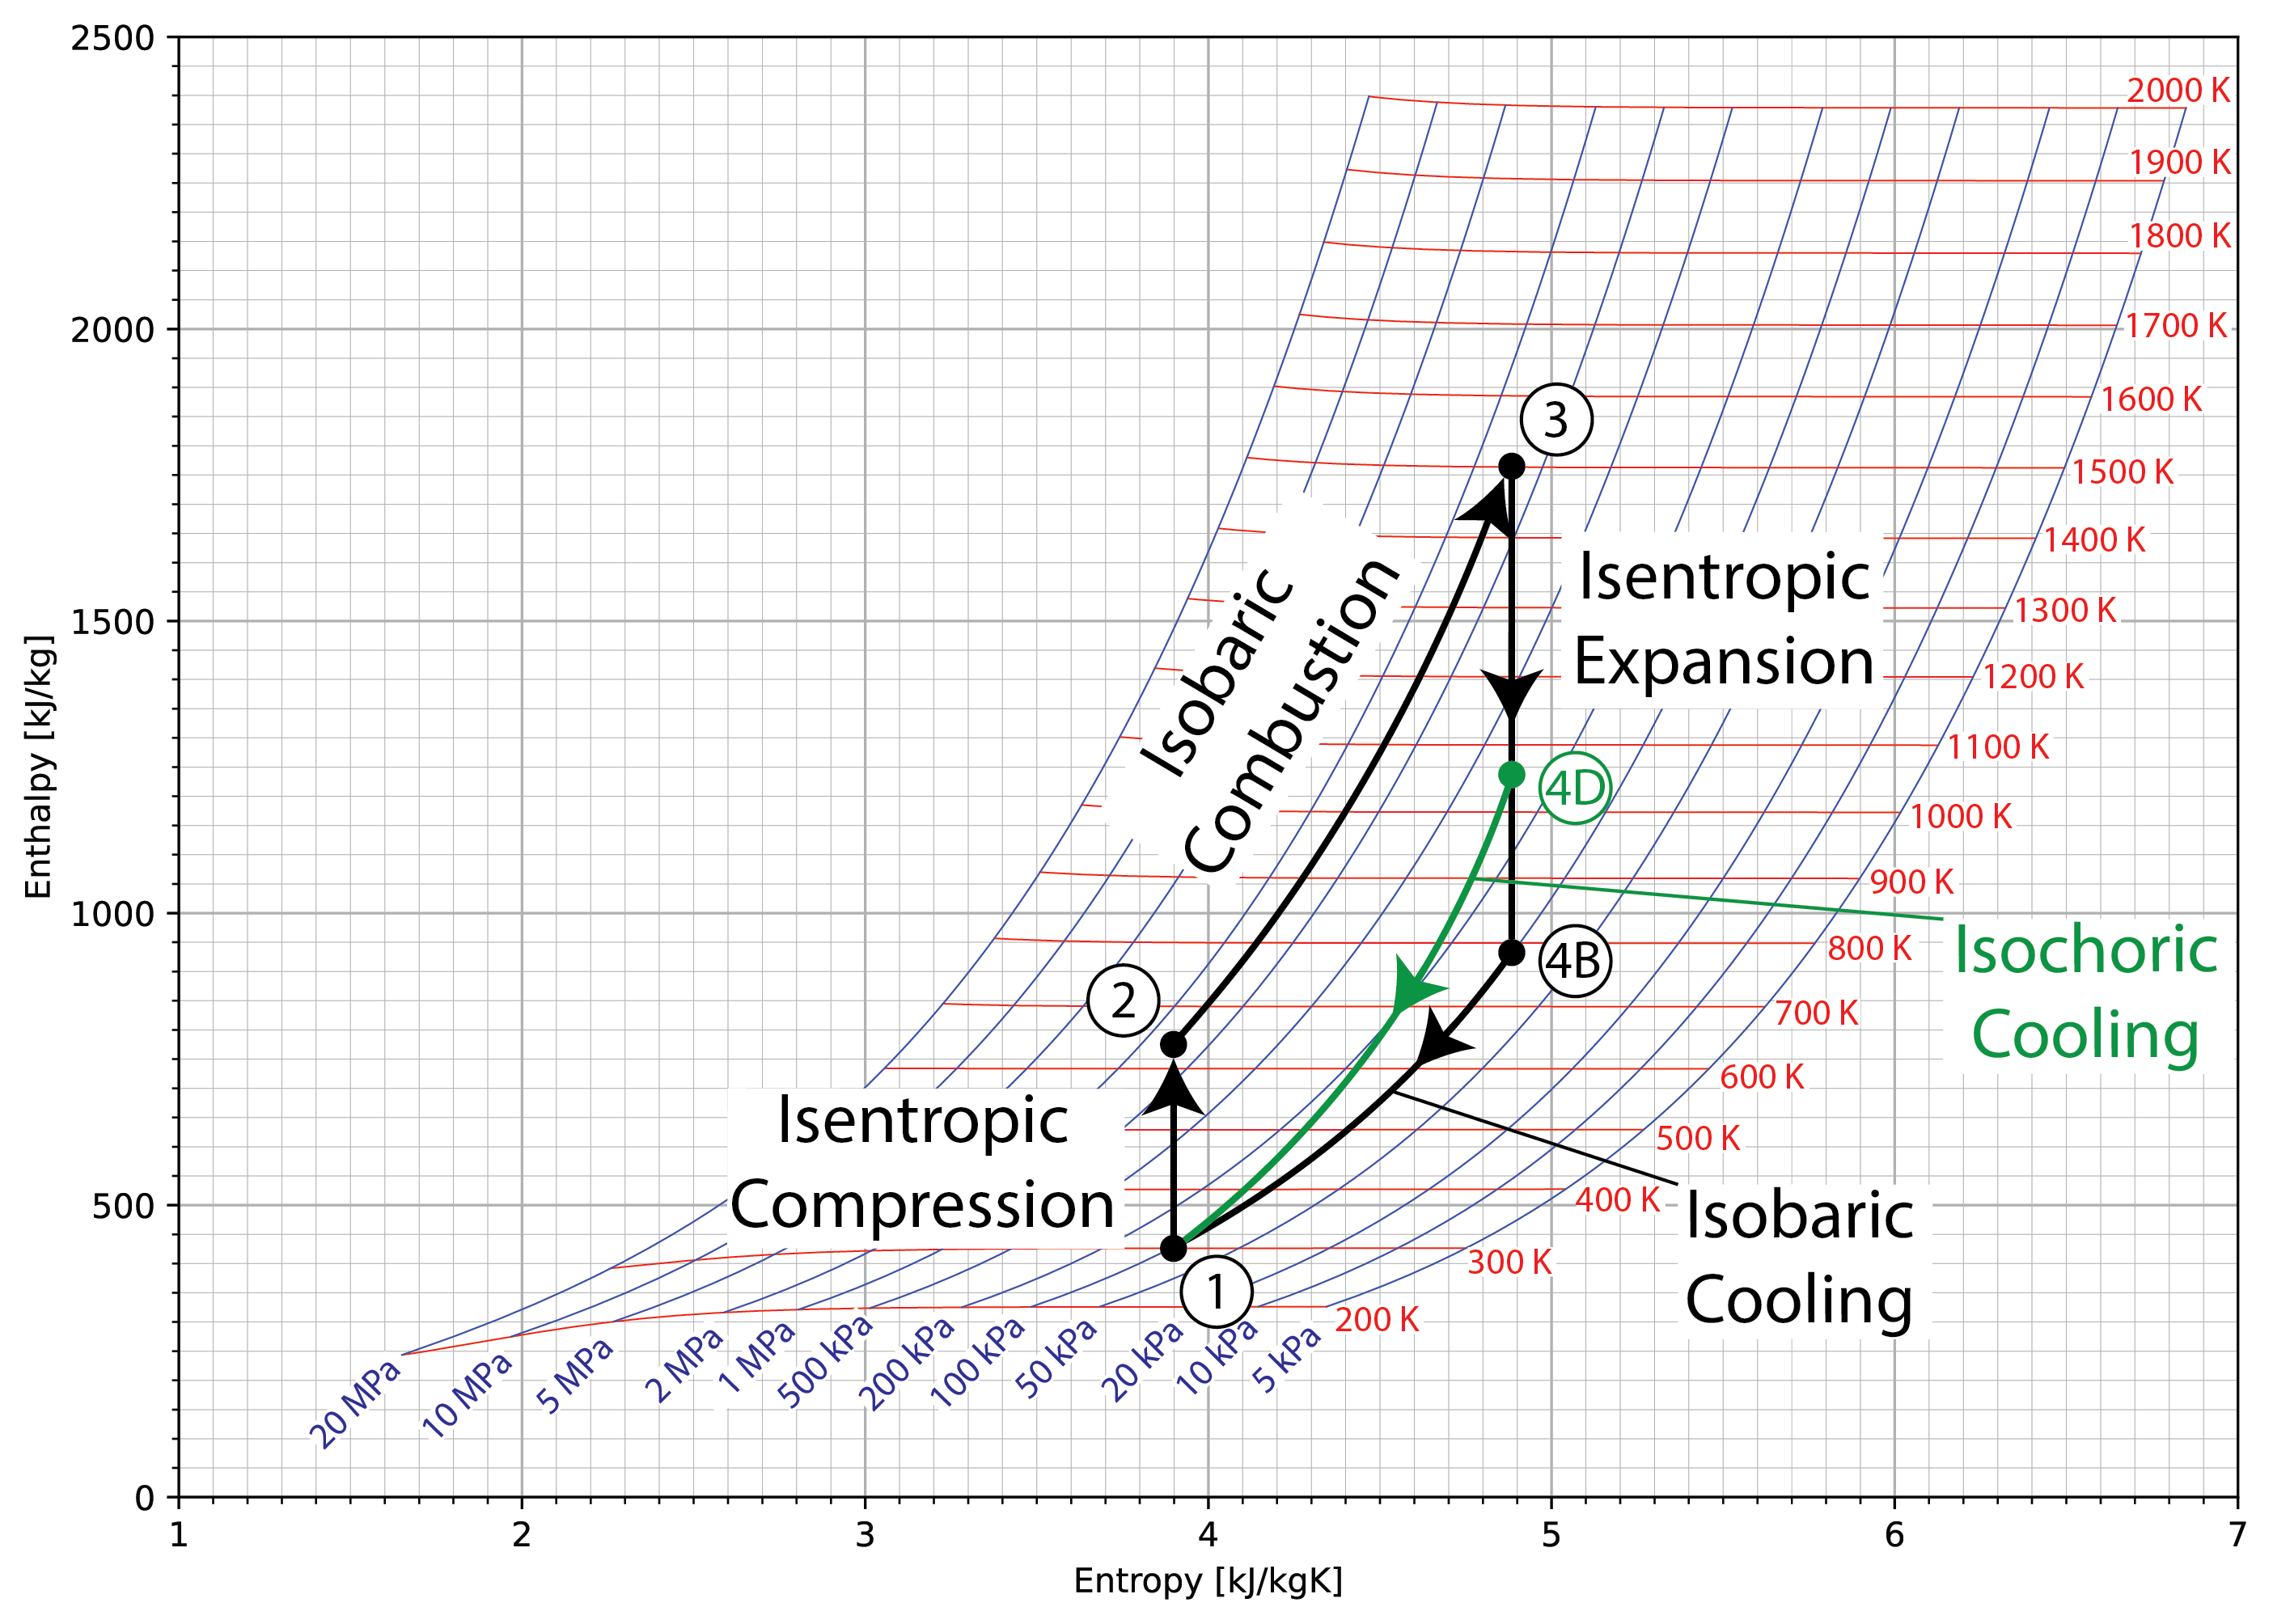
\includegraphics[width=.95\linewidth]{BraytonDieselhs}
  %\caption{Section view schematic of GE T700 engine.}
  %\label{fig:t700_section}
\end{subfigure}
\caption{The Brayton and Diesel cycles plotted on the $p$-$v$ (left) and a $h$-$s$ (right) diagrams.  The Diesel cycle is plotted in green when it diverges from the Brayton cycle.}
\label{fig:BraytonDieselComp}
\end{figure}

The primary difference comes from the state after expansion.  For the Diesel cycle, the assumption is that the volume will be equal between states 1 and 4, but the pressures are different.  For the Brayton cycle, the pressures are equal, with different volumes.  Maintaining the Brayton cycle in a piston requires a significant amount of added complexity.  As such, the Brayton cycle is better suited for open systems, while the Diesel cycle is more suitable for closed systems.

Note the additional amount of work generated in the expansion of the Brayton cycle.  Assuming that the compression ratio is the same and the maximum temperature is the same between the two cycles, the Brayton cycle will have significantly higher efficiency.

\subsection{Basic Brayton Cycle}
%--------------------------------------------------------------------
The basic Brayton cycle is quite simple (composed of only three components), but as with the Rankine cycle, has the potential for a large variety of modifications.
The basic Brayton cycle has the following components:

\begin{itemize}
\item A compressor - does work on the air and increases the enthalpy and pressure.
\item A combustion chamber (or combustor) - adds energy to the air as heat at constant pressure.
\item A turbine - extracts energy from the air as work while reducing the pressure.
\end{itemize}

Figure \ref{fig:turboshaft} shows a fairly standard arrangement of a gas generator engine.  Cutaway views of actual gas generators can be seen on \href{https://www.ge.com/gas-power/products/gas-turbines}{GE's website}.
\begin{figure}[H]
  \centering
  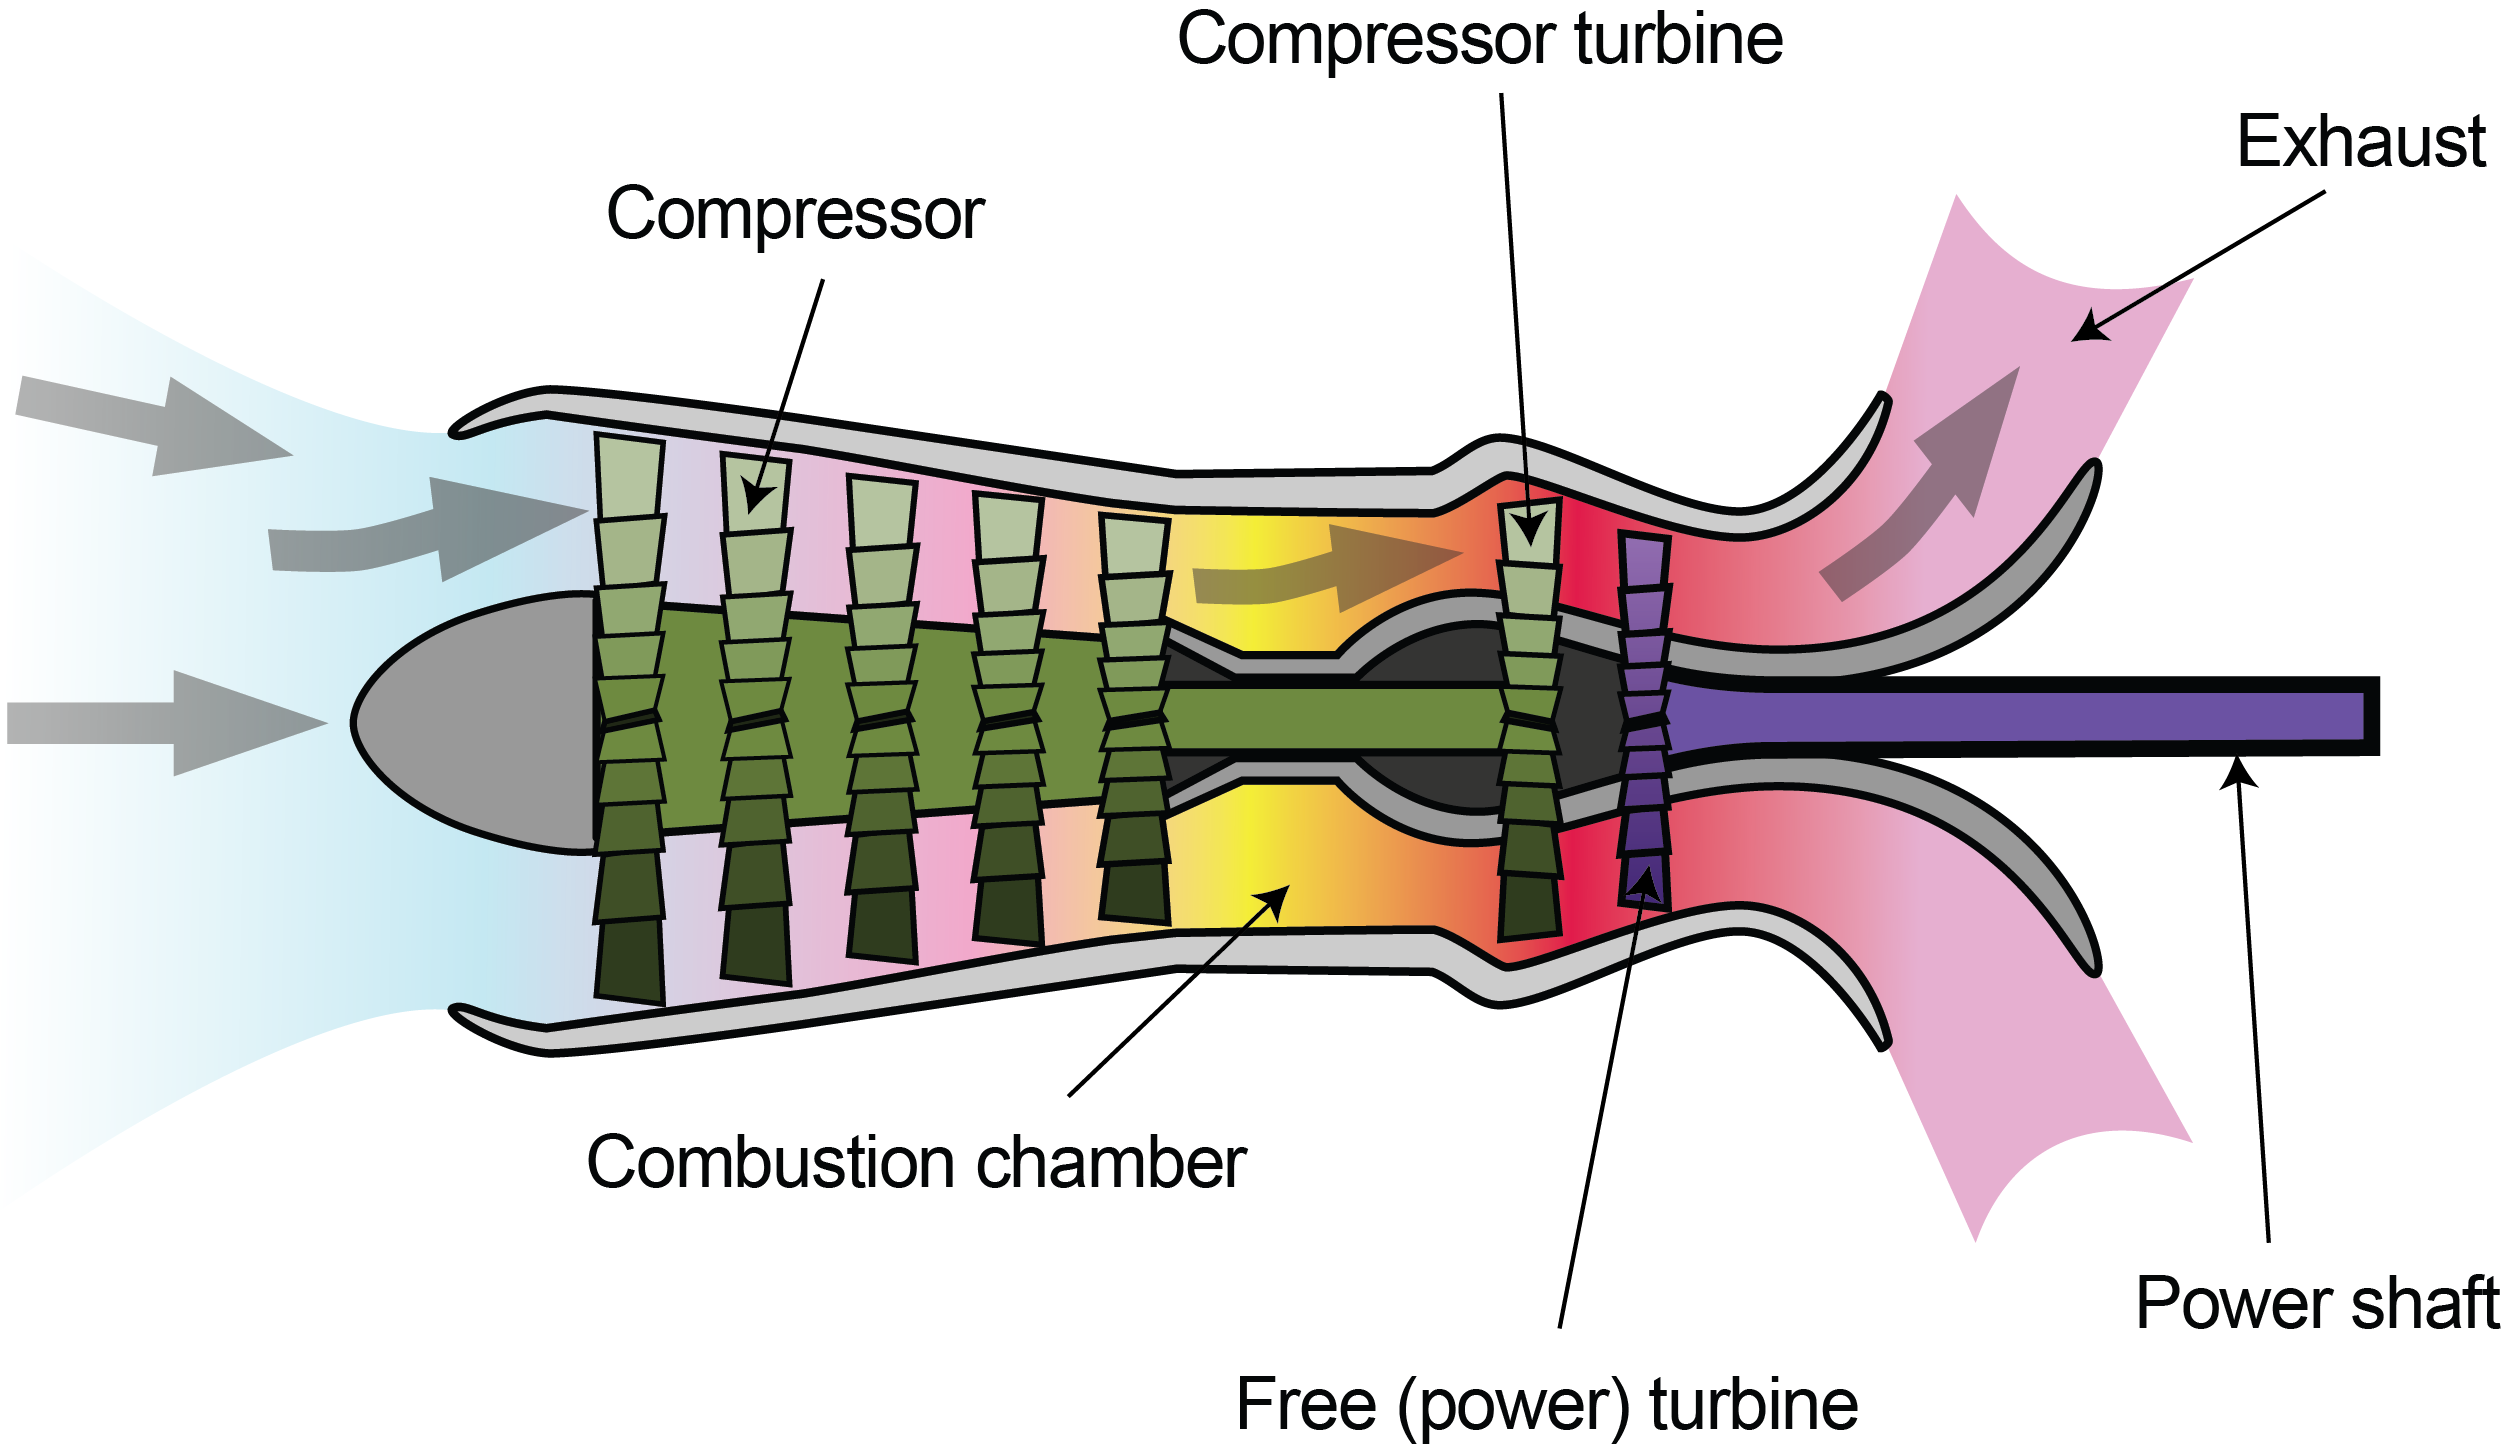
\includegraphics[width=.7\linewidth]{turboshaftDiagram}
  \caption{A diagram showing the various components of a gas generator engine, which uses the Brayton Cycle. Credit: Mliu92, \href{https://commons.wikimedia.org/wiki/File:Turboshaft_operation_(multilanguage).svg}{Wikipedia}.}
  \label{fig:turboshaft}
\end{figure}

Air is typically used as the working fluid, as it is easily accessible and free to use.  Figure \ref{fig:turboshafths} shows the cycle on an $h$-$s$ diagram.  The cooling process which was present in Figure \ref{fig:BraytonDieselComp} is typically omitted, as the exhaust gas is vented, rather than being reused.

\begin{figure}[H]
  \centering
  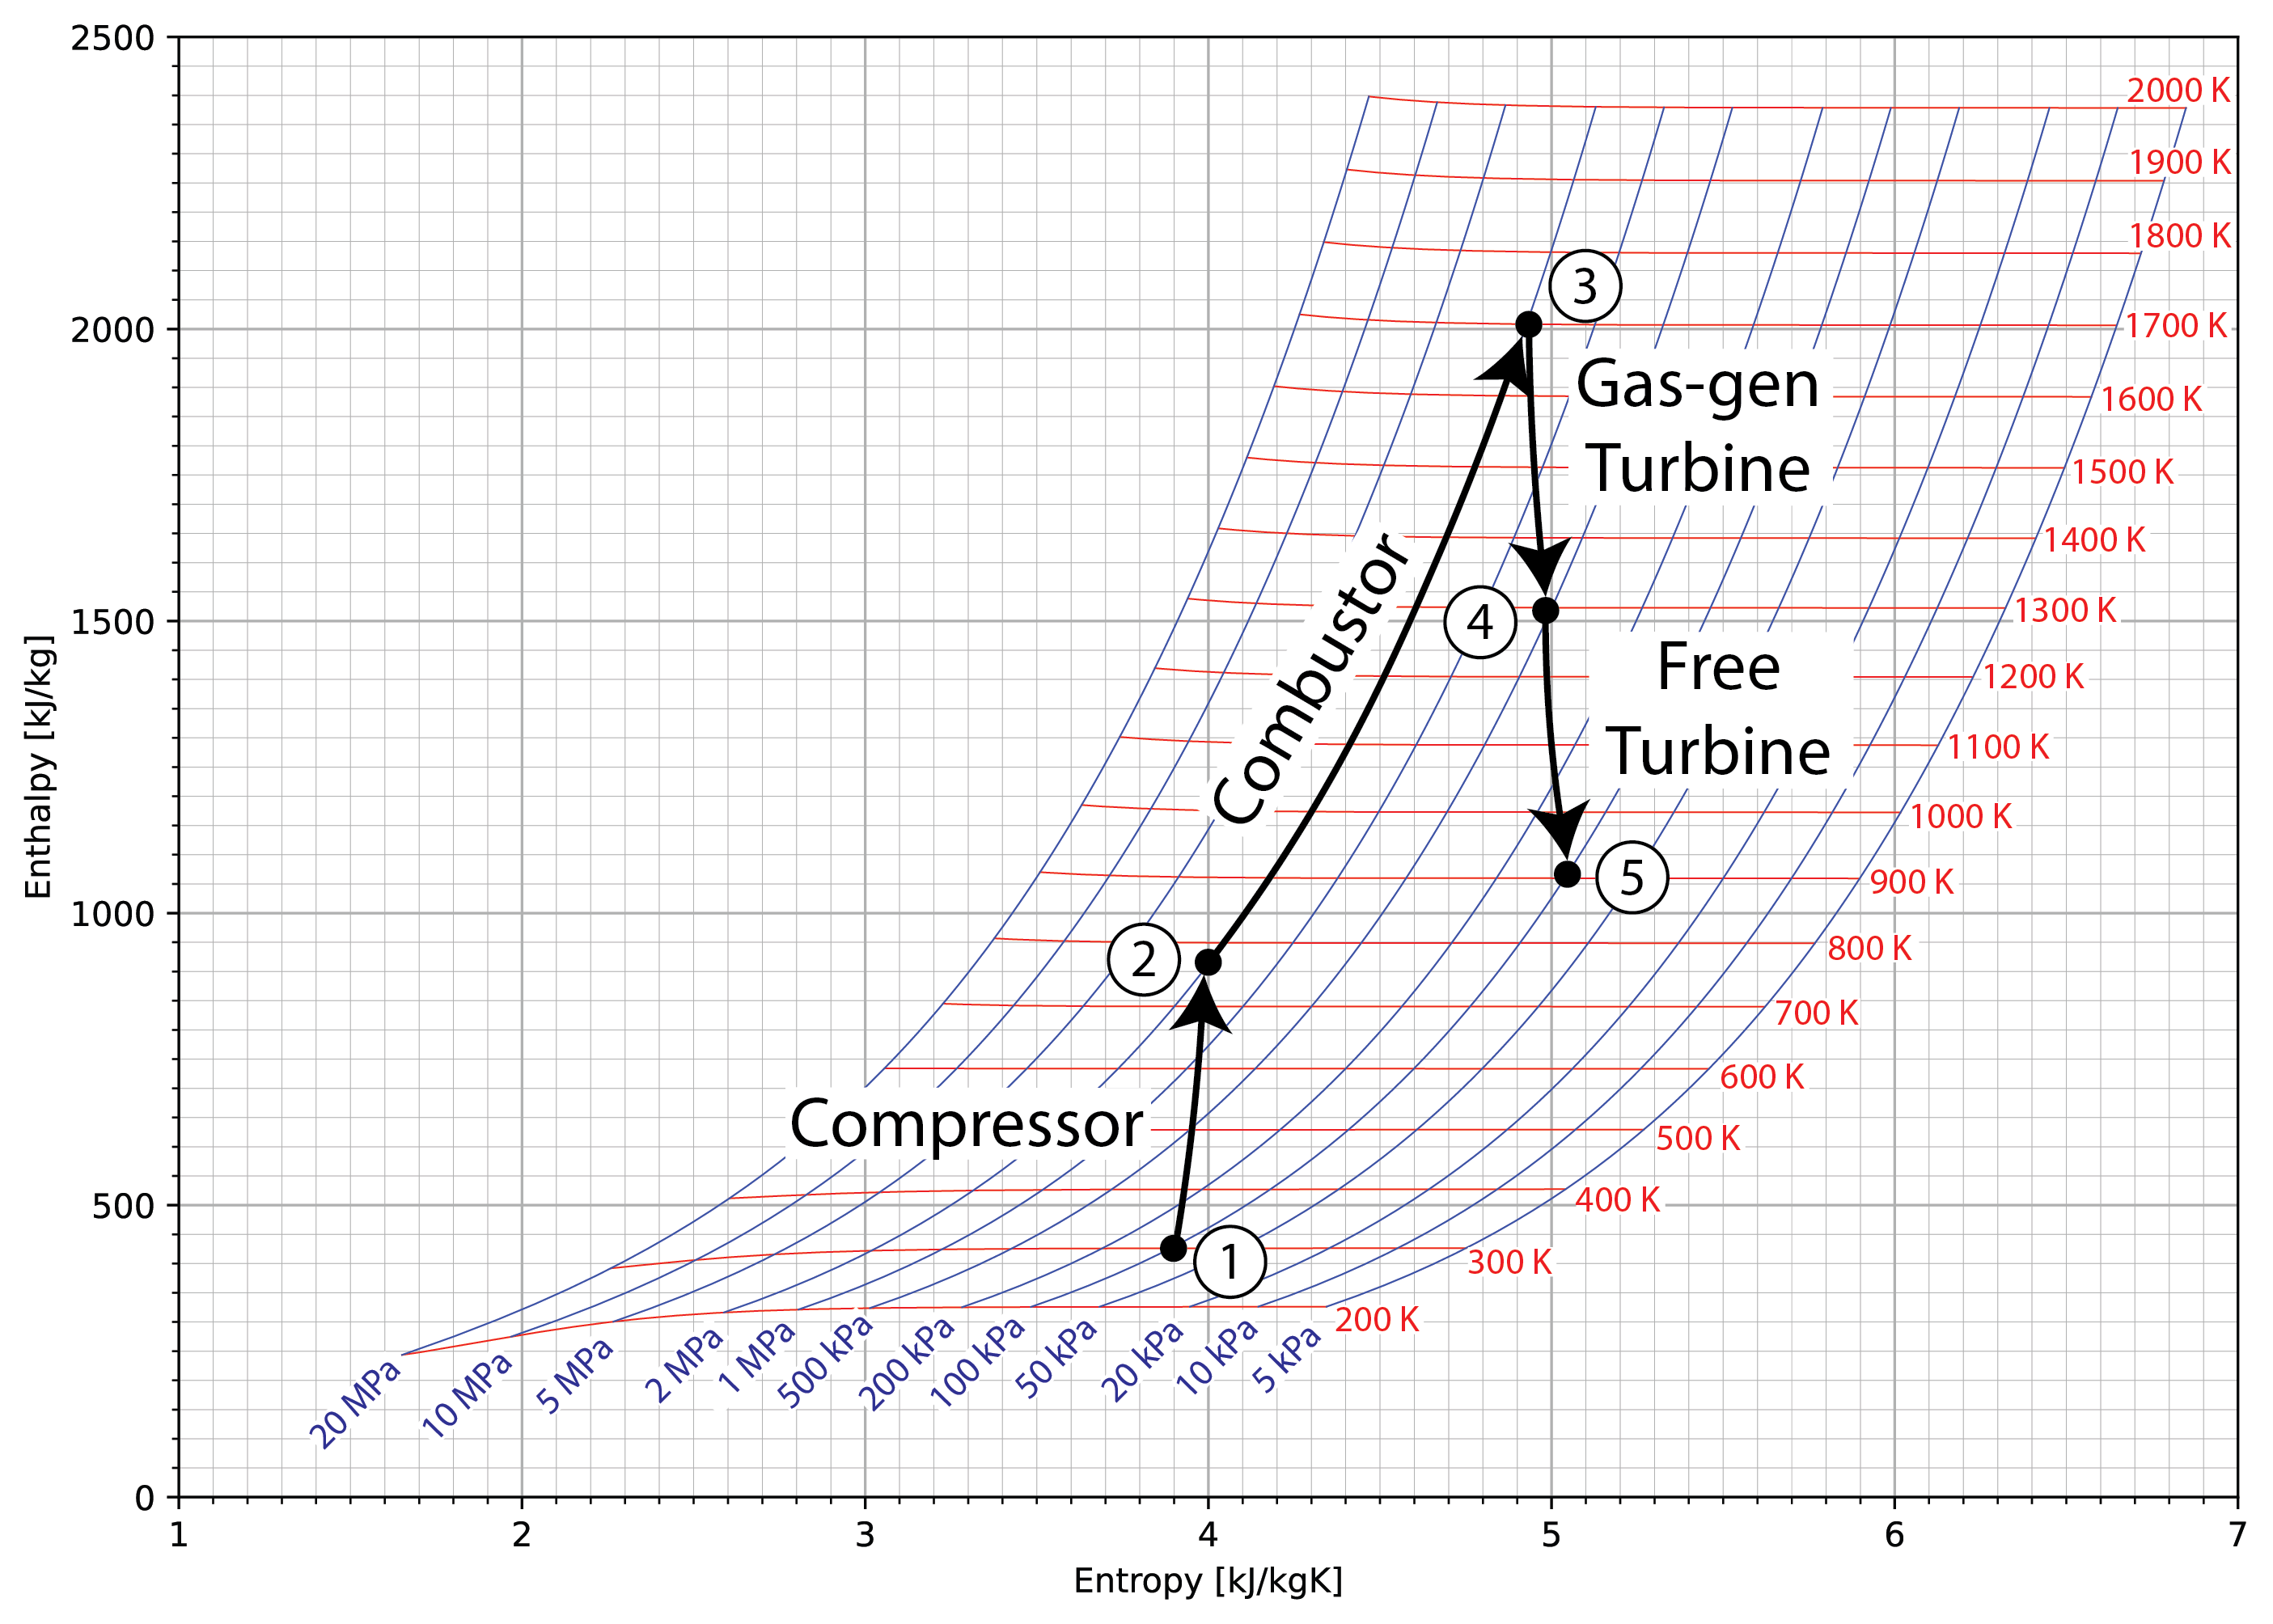
\includegraphics[width=.7\linewidth]{gasgenhs}
  \caption{An example Brayton cycle plotted on the $h$-$s$ diagram for air.}
  \label{fig:turboshafths}
\end{figure}

Example \ref{ex:turboshaft} looks at power generation from a Brayton cycle.


\begin{example}[label=ex:turboshaft]{Brayton Cycle Power Generation}
  A Brayton cycle gas generator intakes air at 300 K and 100 kPa.  The compressor has a pressure ratio of 15, and the gas-generator turbine has an inlet temperature of 1500 K. The compressor and both turbines are isentropic.  

  \begin{enumerate}[a)]
  \item Plot each state and process on the $h$-$s$ diagram for air.
  \item Determine the temperature, pressure, enthalpy, and entropy of each state.
  \item Find the work/heat transfer of each component.
  \item Determine the efficiency of the gas generator.
  \end{enumerate}

  \subsubsection*{$h$-$s$ Diagram}
  The $h$-$s$ diagram is relatively straightforward for ideal cycles, as the compressor and turbines can be represented as vertical lines.  We can find each of the states as follows:
  \begin{itemize}
  \item {\bf State 1 - } The intersection of 300 K and 100 kPa
  \item {\bf State 2 - } Directly above state 1, at 1.5 MPa (from the pressure ratio of 15)
  \item {\bf State 3 - } The intersection of 1500 K and 1.5 MPa
  \item {\bf State 4 - } Directly below state 3, with the same enthalpy change as the compressor
  \item {\bf State 5 - } Directly below state 4, at a pressure of 100 kPa
  \end{itemize}

  \begin{center}
    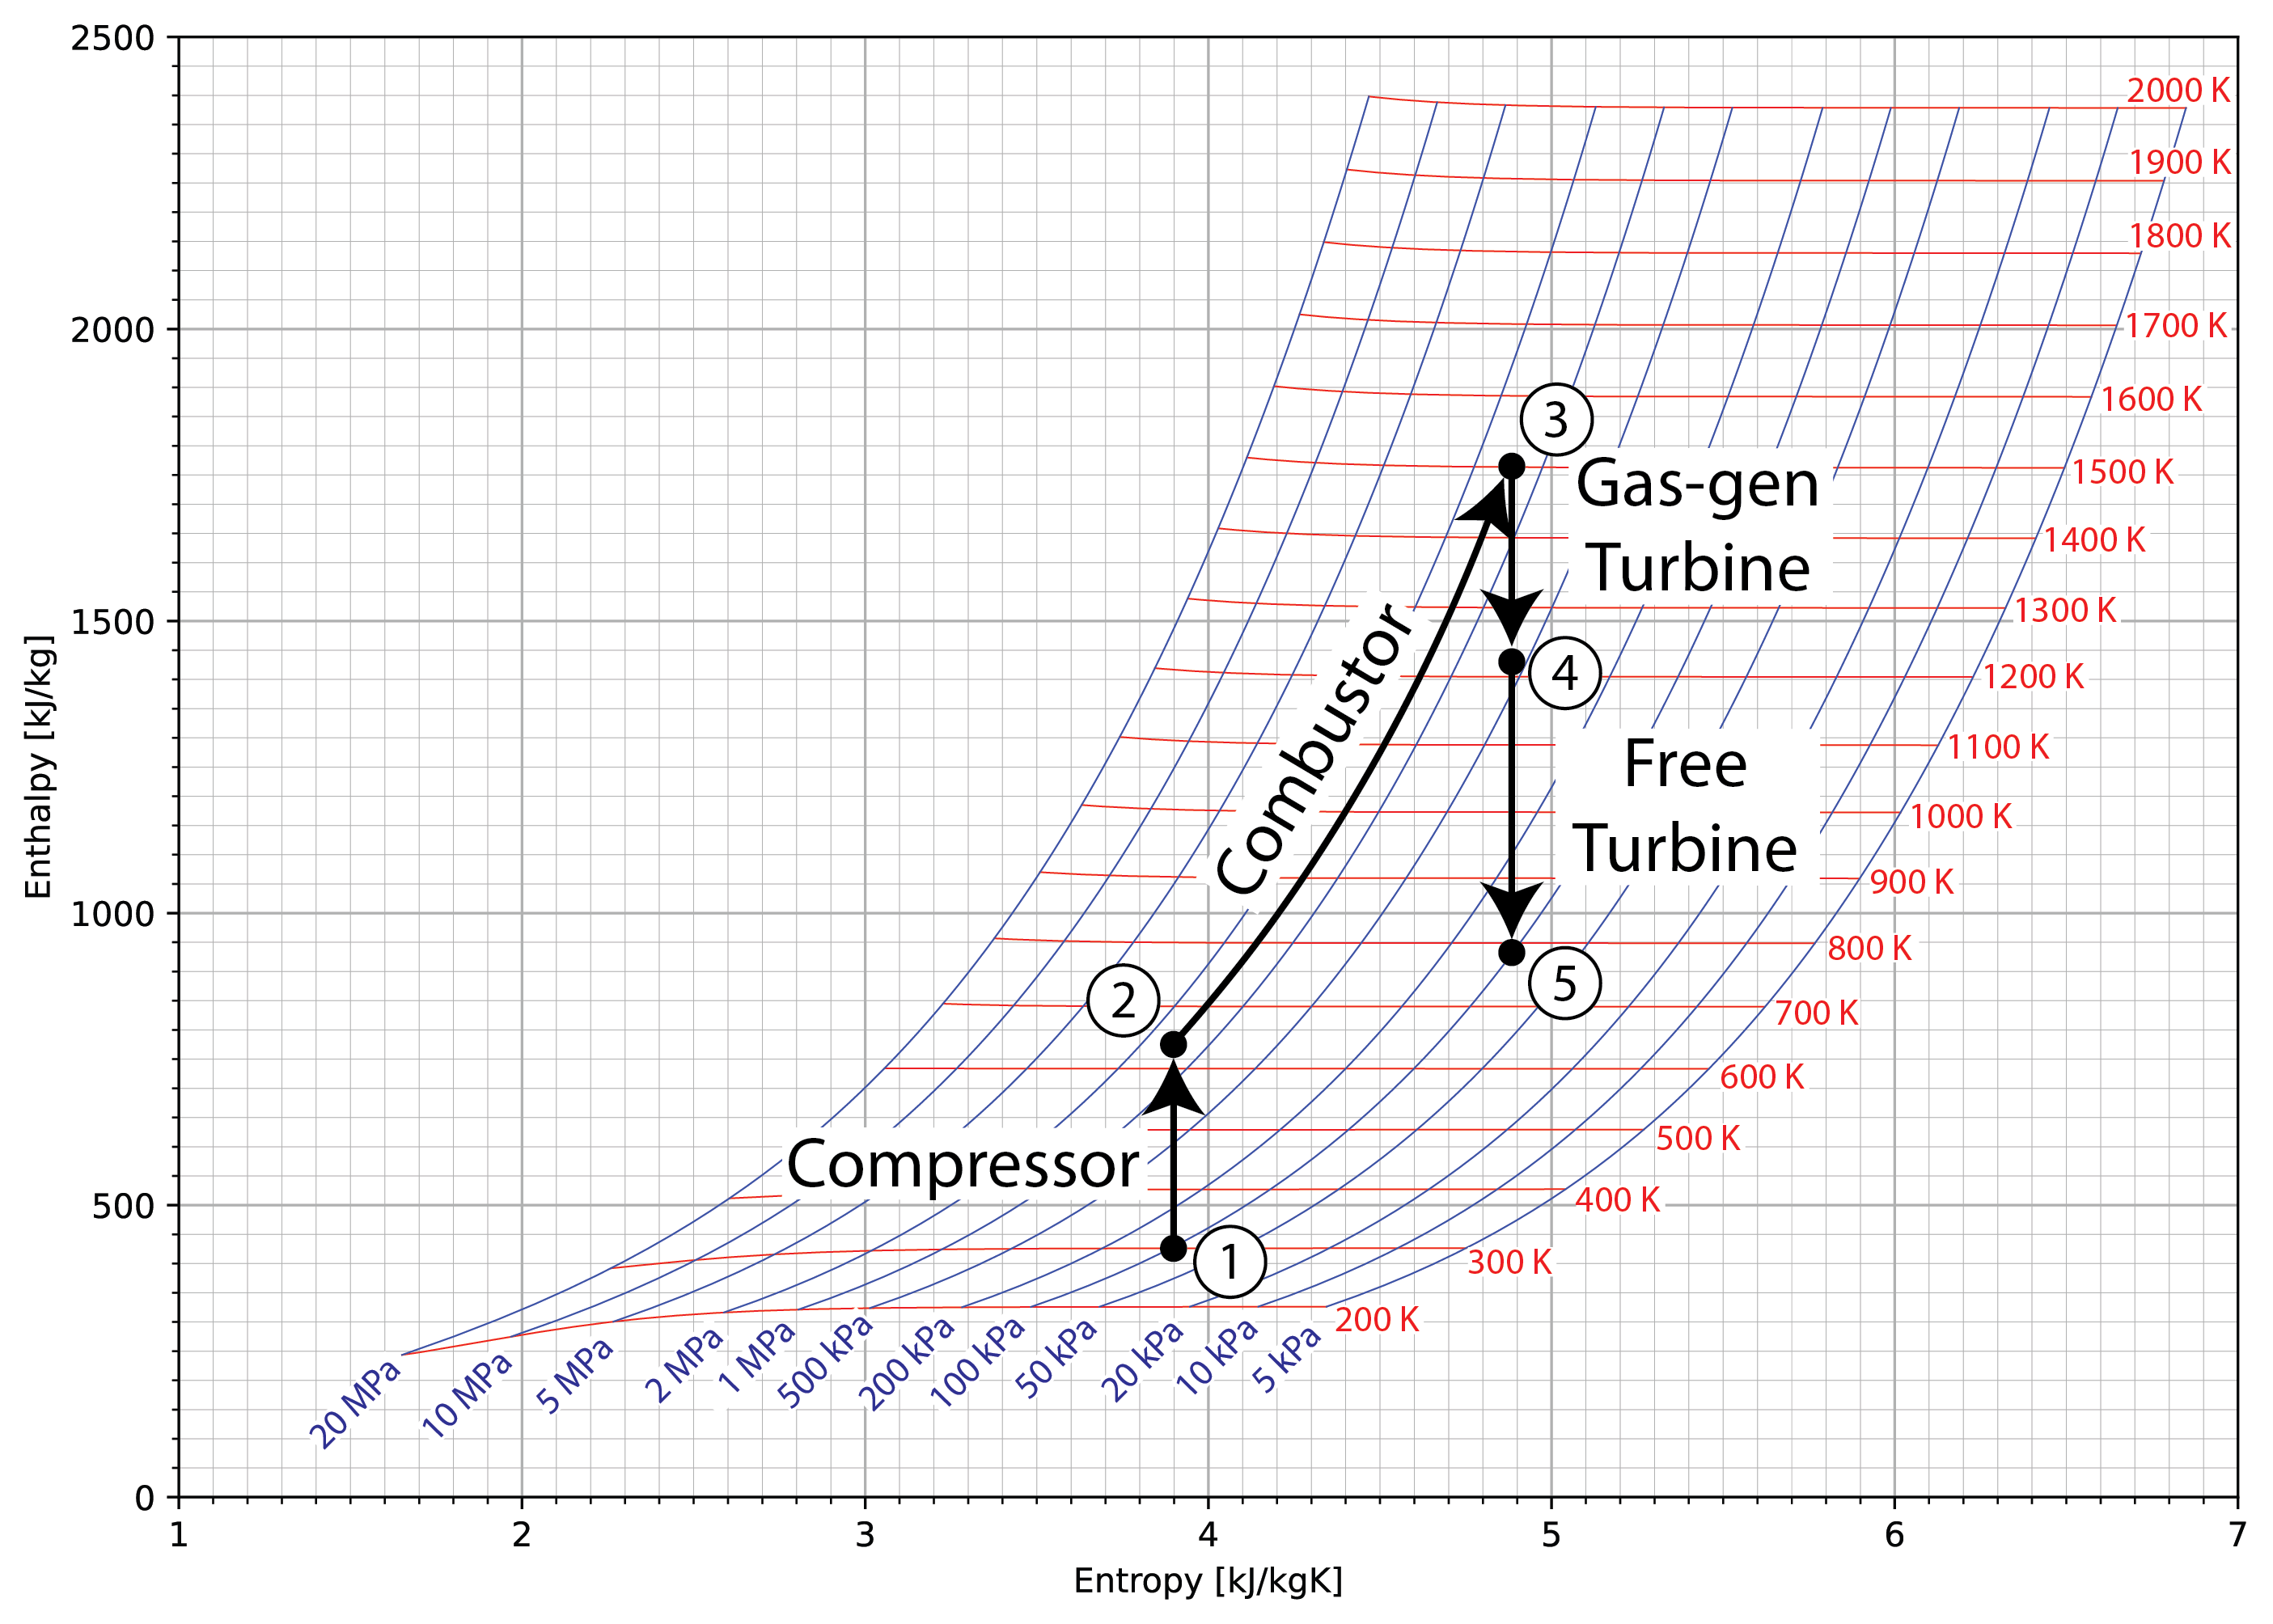
\includegraphics[width=.8\linewidth]{gasGenExamplehs}
  \end{center}

  
  \subsubsection*{Properties}

  Because the compressor and turbines are isentropic, we can find the entropy at states 1 and 3, and copy those values to the other states.  Values in black are given, while values in red are found from CoolProp.
  
  \begin{table}[H]
    \centering
    \def\arraystretch{1.5}
    \begin{tabular}{r|cccc}
      State & Pressure & Temperature & Enthalpy & Entropy \\ \hline
      1 & 100 kPa & 300 K &  & {\color{Red} 3.891 $\frac{\rm kJ}{\rm kg\, K}$} \\
      2 & 1.5 MPa &  &  & {\color{Red} 3.891 $\frac{\rm kJ}{\rm kg\, K}$} \\
      3 & 1.5 MPa & 1500 K & & {\color{Red} 4.857 $\frac{\rm kJ}{\rm kg\, K}$} \\
      4 &  &  & & {\color{Red} 4.857 $\frac{\rm kJ}{\rm kg\, K}$} \\
      5 & 100 kPa &  & & {\color{Red} 4.857 $\frac{\rm kJ}{\rm kg\, K}$}
    \end{tabular}
    \def\arraystretch{1.0}
  \end{table}
  
  This is enough to give us values for everything except for state 4.  Again, new values are in red.
  
  \begin{table}[H]
    \centering
    \def\arraystretch{1.5}
    \begin{tabular}{r|cccc}
      State & Pressure & Temperature & Enthalpy & Entropy \\ \hline
      1 & 100 kPa & 300 K & {\color{Red} 426.3 $\frac{\rm kJ}{\rm kg}$} & 3.891 $\frac{\rm kJ}{\rm kg\, K}$ \\
      2 & 1.5 MPa & {\color{Red} 641 K} & {\color{Red} 777.5 $\frac{\rm kJ}{\rm kg}$} & 3.891 $\frac{\rm kJ}{\rm kg\, K}$ \\
      3 & 1.5 MPa & 1500 K & {\color{Red} 1763.6 $\frac{\rm kJ}{\rm kg}$} & 4.857 $\frac{\rm kJ}{\rm kg\, K}$ \\
      4 &  &  &  & 4.857 $\frac{\rm kJ}{\rm kg\, K}$ \\
      5 & 100 kPa & {\color{Red} 764 K} &  {\color{Red} 909.1 $\frac{\rm kJ}{\rm kg}$} & 4.857 $\frac{\rm kJ}{\rm kg\, K}$
    \end{tabular}
    \def\arraystretch{1.0}
  \end{table}
  
  Finally, the enthalpy of state 4 is determined by the relationship $w_{turb, gg} = w_{comp}$.
  
  \begin{equation*}
    h_4 = h_3 - (h_2 - h_1) =  1763.6\, \frac{\rm kJ}{\rm kg} - \left(777.5\, \frac{\rm kJ}{\rm kg} - 426.3\, \frac{\rm kJ}{\rm kg}\right) = 1412.4\, \frac{\rm kJ}{\rm kg}
  \end{equation*}
  
  Along with the entropy, this gives us enough information to finish the table.
  
  \begin{table}[H]
    \centering
    \def\arraystretch{1.5}
    \begin{tabular}{r|cccc}
      State & Pressure & Temperature & Enthalpy & Entropy \\ \hline
      1 & 100 kPa & 300 K & 426.3 $\frac{\rm kJ}{\rm kg}$ & 3.891 $\frac{\rm kJ}{\rm kg\, K}$ \\
      2 & 1.5 MPa & 641 K & 777.5 $\frac{\rm kJ}{\rm kg}$ & 3.891 $\frac{\rm kJ}{\rm kg\, K}$ \\
      3 & 1.5 MPa & 1500 K & 1763.6 $\frac{\rm kJ}{\rm kg}$ & 4.857 $\frac{\rm kJ}{\rm kg\, K}$ \\
      4 &  {\color{Red} 607 kPa} &  {\color{Red} 1206.7 K} &  {\color{Red} 1412.4 $\frac{\rm kJ}{\rm kg}$}  & 4.857 $\frac{\rm kJ}{\rm kg\, K}$ \\
      5 & 100 kPa & 764 K & 909.1 $\frac{\rm kJ}{\rm kg}$ & 4.857 $\frac{\rm kJ}{\rm kg\, K}$
    \end{tabular}
    \def\arraystretch{1.0}
  \end{table}
  
  \subsubsection*{Work, Heat Transfer, and Efficiency}
  As typical for open systems, finding the work and heat transfer for individual components is done simply by finding the change in enthalpy.  Thus, the work extracted from the free turbine and the heat transfer in the combustor are as follows:
  \begin{align*}
    w_{turb, free} &= h_4 - h_5 = 1412.4\, \frac{\rm kJ}{\rm kg} - 909.1\, \frac{\rm kJ}{\rm kg} = 503.3\, \frac{\rm kJ}{\rm kg} \\
    q_{comb} &= h_3 - h_2 = 1763.6\, \frac{\rm kJ}{\rm kg} - 777.5\, \frac{\rm kJ}{\rm kg} = \redbox{986.1\, \frac{\rm kJ}{\rm kg}}
  \end{align*}

  Because the work of the gas generator turbine and the compressor are equal, they will cancel out in the efficiency equation.  Without those two terms, the efficiency is simply:
  \begin{equation*}
    \eta_{th} = \frac{w_{turb, free}}{q_{comb}} = \frac{503.3\, \frac{\rm kJ}{\rm kg}}{986.1\, \frac{\rm kJ}{\rm kg}} = 0.51 = \redbox{51 \%}
  \end{equation*}

  Thus, the gas generator with ideal components has an efficiency of 51\%.
  
\end{example}

\subsection{Combined Cycle}
%--------------------------------------------------------------------
The waste heat of a gas generator tends to be at a much higher temperature than we are used to from engines.  Because of this, it can be used to power a Rankine cycle, in what is known as a {\bf combined cycle}.  Because the waste energy is essentially free, the paired Rankine cycle can only increase the overall efficiency of the two cycles.  Example \ref{ex:combinedCycle} examines a combined cycle to determine its overall efficiency.

\begin{example}[label=ex:combinedCycle]{Combined Cycle Efficiency}
  Using the results from Example \ref{ex:turboshaft}, consider pairing the Rankine cycle from Example \ref{ex:RankineReheat}, which was calculated to have an efficiency of 25.5\%.  Assume that the gas generator provides 10 MW of power on its own, and that the water in the boiler of the Rankine cycle can cool the air to a temperature of 400 K.
  
  \begin{enumerate}[a)]
  \item Determine the mass flow rate of air through the gas generator.
  \item Determine the total heat transfer into the boiler.
  \item Determine the work output of the Rankine cycle.
  \item Determine the overall efficiency of the combined cycle.
  \end{enumerate}

  \subsubsection*{Mass Flow Rate of Air}
  The mass flow rate can be found with the relationship $\dot{W} = \dot{m} w$, based on the free turbine:
  \begin{equation*}
    \dot{m} = \frac{\dot{W}_{turb, free}}{w_{turb, free}} = \frac{10\, {\rm MW}}{503.3\, \frac{\rm kJ}{\rm kg}} = \redbox{19.9\, \frac{\rm kg}{\rm s}}
  \end{equation*}

  \subsubsection*{Rankine Heat Transfer and Work}
  Let's take a look at the $h$-$s$ diagram for the gas generator again, this time adding heat transfer out of the air after gas generator turbine.

  \begin{center}
    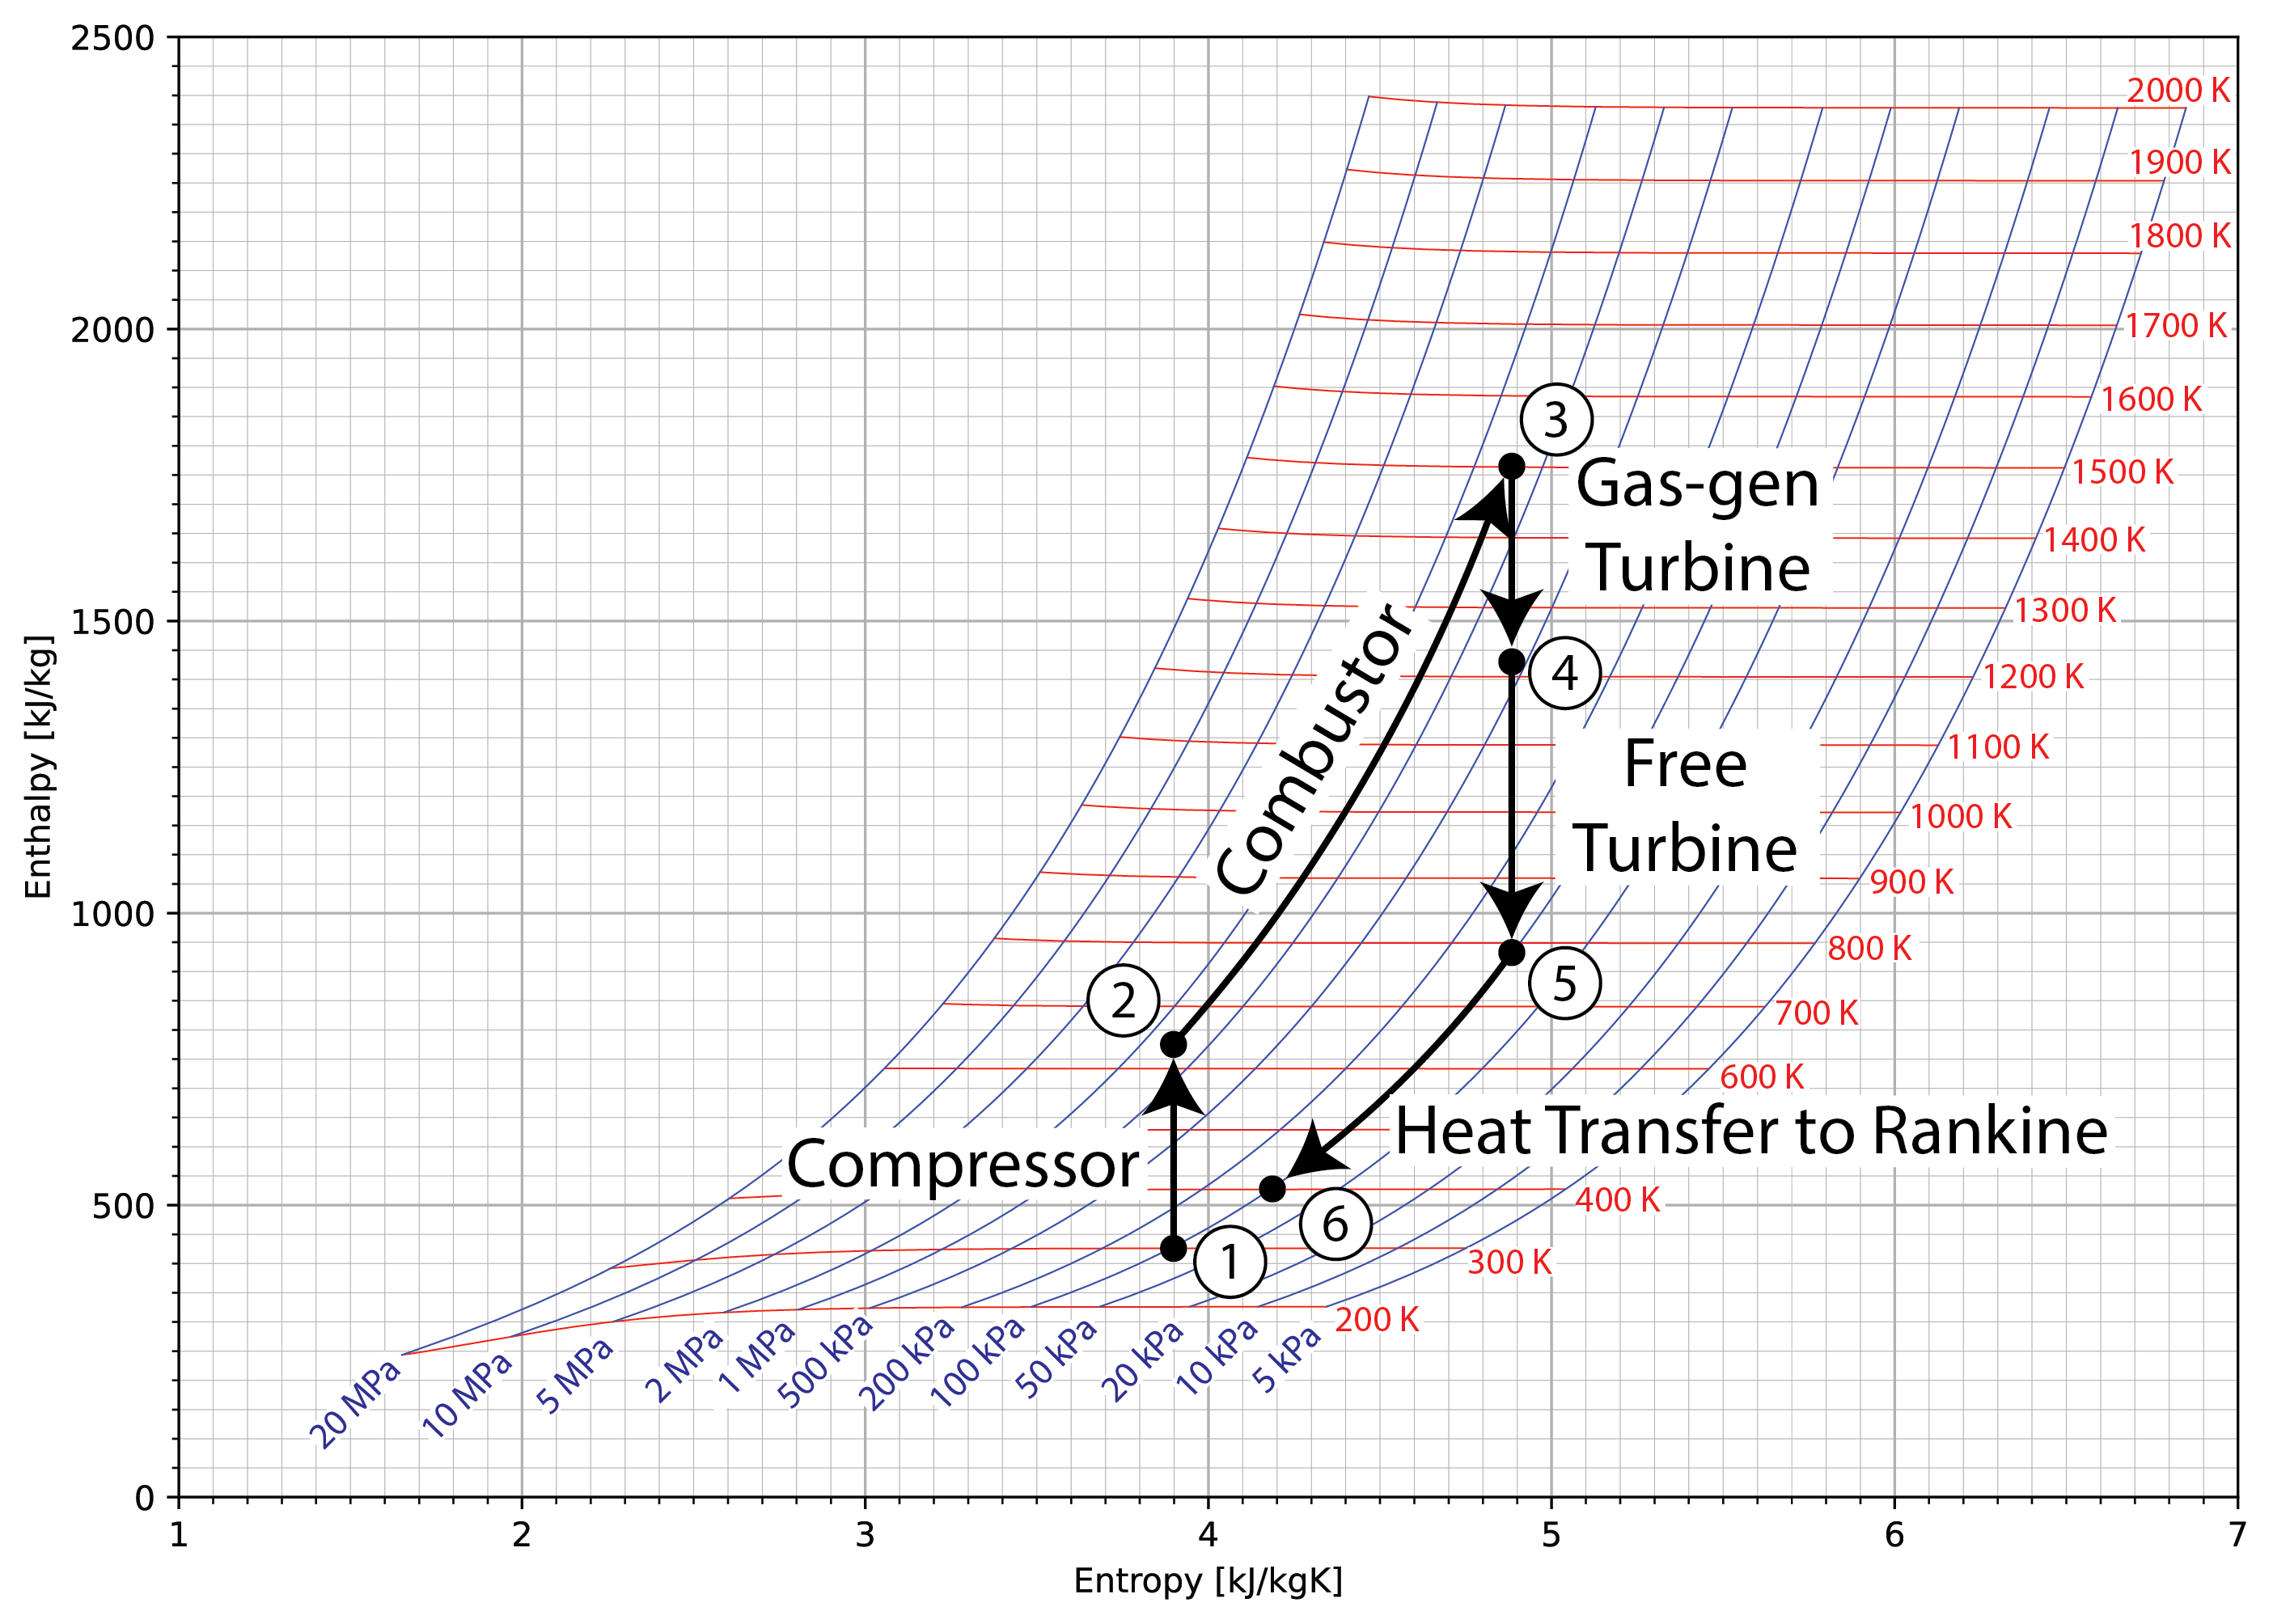
\includegraphics[width=.8\linewidth]{gasGenExamplehs2}
  \end{center}
  The exact value for enthalpy after the heat transfer is 527.3\,$\frac{\rm kJ}{\rm kg}$, found from the pressure and temperature at state 6.  Now that $h_6$ is known, the heat transfer to the Rankine cycle can be determined by the enthalpy drop in the air:
  \begin{equation*}
    \dot{Q}_{R} = \dot{m} (h_5-h_6) = 19.9\, \frac{\rm kg}{\rm s} \left(909.1\, \frac{\rm kJ}{\rm kg} - 527.3\, \frac{\rm kJ}{\rm kg}\right) = \redbox{7.59\, {\rm MW}}
  \end{equation*}

  Using the efficiency of the Rankine cycle, we can find the extra work extracted:
  \begin{equation*}
    \dot{W}_{R} = \eta_{th, R}\dot{Q}_{R} = 0.255 \cdot 7.59\, {\rm MW} = \redbox{1.94\, {\rm MW}}
  \end{equation*}
  \subsubsection*{Overall Efficiency}
  The overall efficiency of the combined cycle is determined by the sum of all power generated divided by the total heat flow into the gas generator.  The heat flow into the Rankine cycle isn't counted, as it is repurposed waste heat from the Brayton cycle.
  \begin{equation*}
    \eta_{th, CC} = \frac{\dot{W}_{B} + \dot{W}_{R}}{\dot{Q}_{B}} = \frac{10\, {\rm MW} + 1.94\, {\rm MW}}{19.9\, \frac{\rm kg}{\rm s} \cdot 986.1\, \frac{\rm kJ}{\rm kg}} = \frac{11.94\, {\rm MW}}{19.59\, {\rm MW}} = 0.609 = \redbox{60.9\%}
  \end{equation*}

  By adding a Rankine cycle alongside the Brayton cycle to use the waste heat, we end up improving the overall efficiency substantially to almost 61\%.
\end{example}


%====================================================================
\section{Aircraft Engines} \label{sec:aircraft}
%====================================================================

There are many different forms and modifications of aircraft gas turbine engines, and in this course we discuss three variants - the ideal turbojet engine, the more modern turbofan, and the turboprop engine, which is conceptually similar to the engines used for helicopters.

\subsection{Turbojet Engine}
%--------------------------------------------------------------------
The turbojet engine is composed of five components:
\begin{itemize}
\item A diffuser - reduces velocity of incoming flow and transforms kinetic energy into enthalpy.
\item A compressor - does work on the air and increases the enthalpy and pressure.
\item A combustion chamber (or combustor) - adds energy to the air as heat at constant pressure.
\item A turbine - extracts energy from the air as work while reducing the pressure.
\item A nozzle - converts extra enthalpy into kinetic energy while returning the pressure back to atmospheric.
\end{itemize}

\begin{figure}[H]
  \centering
  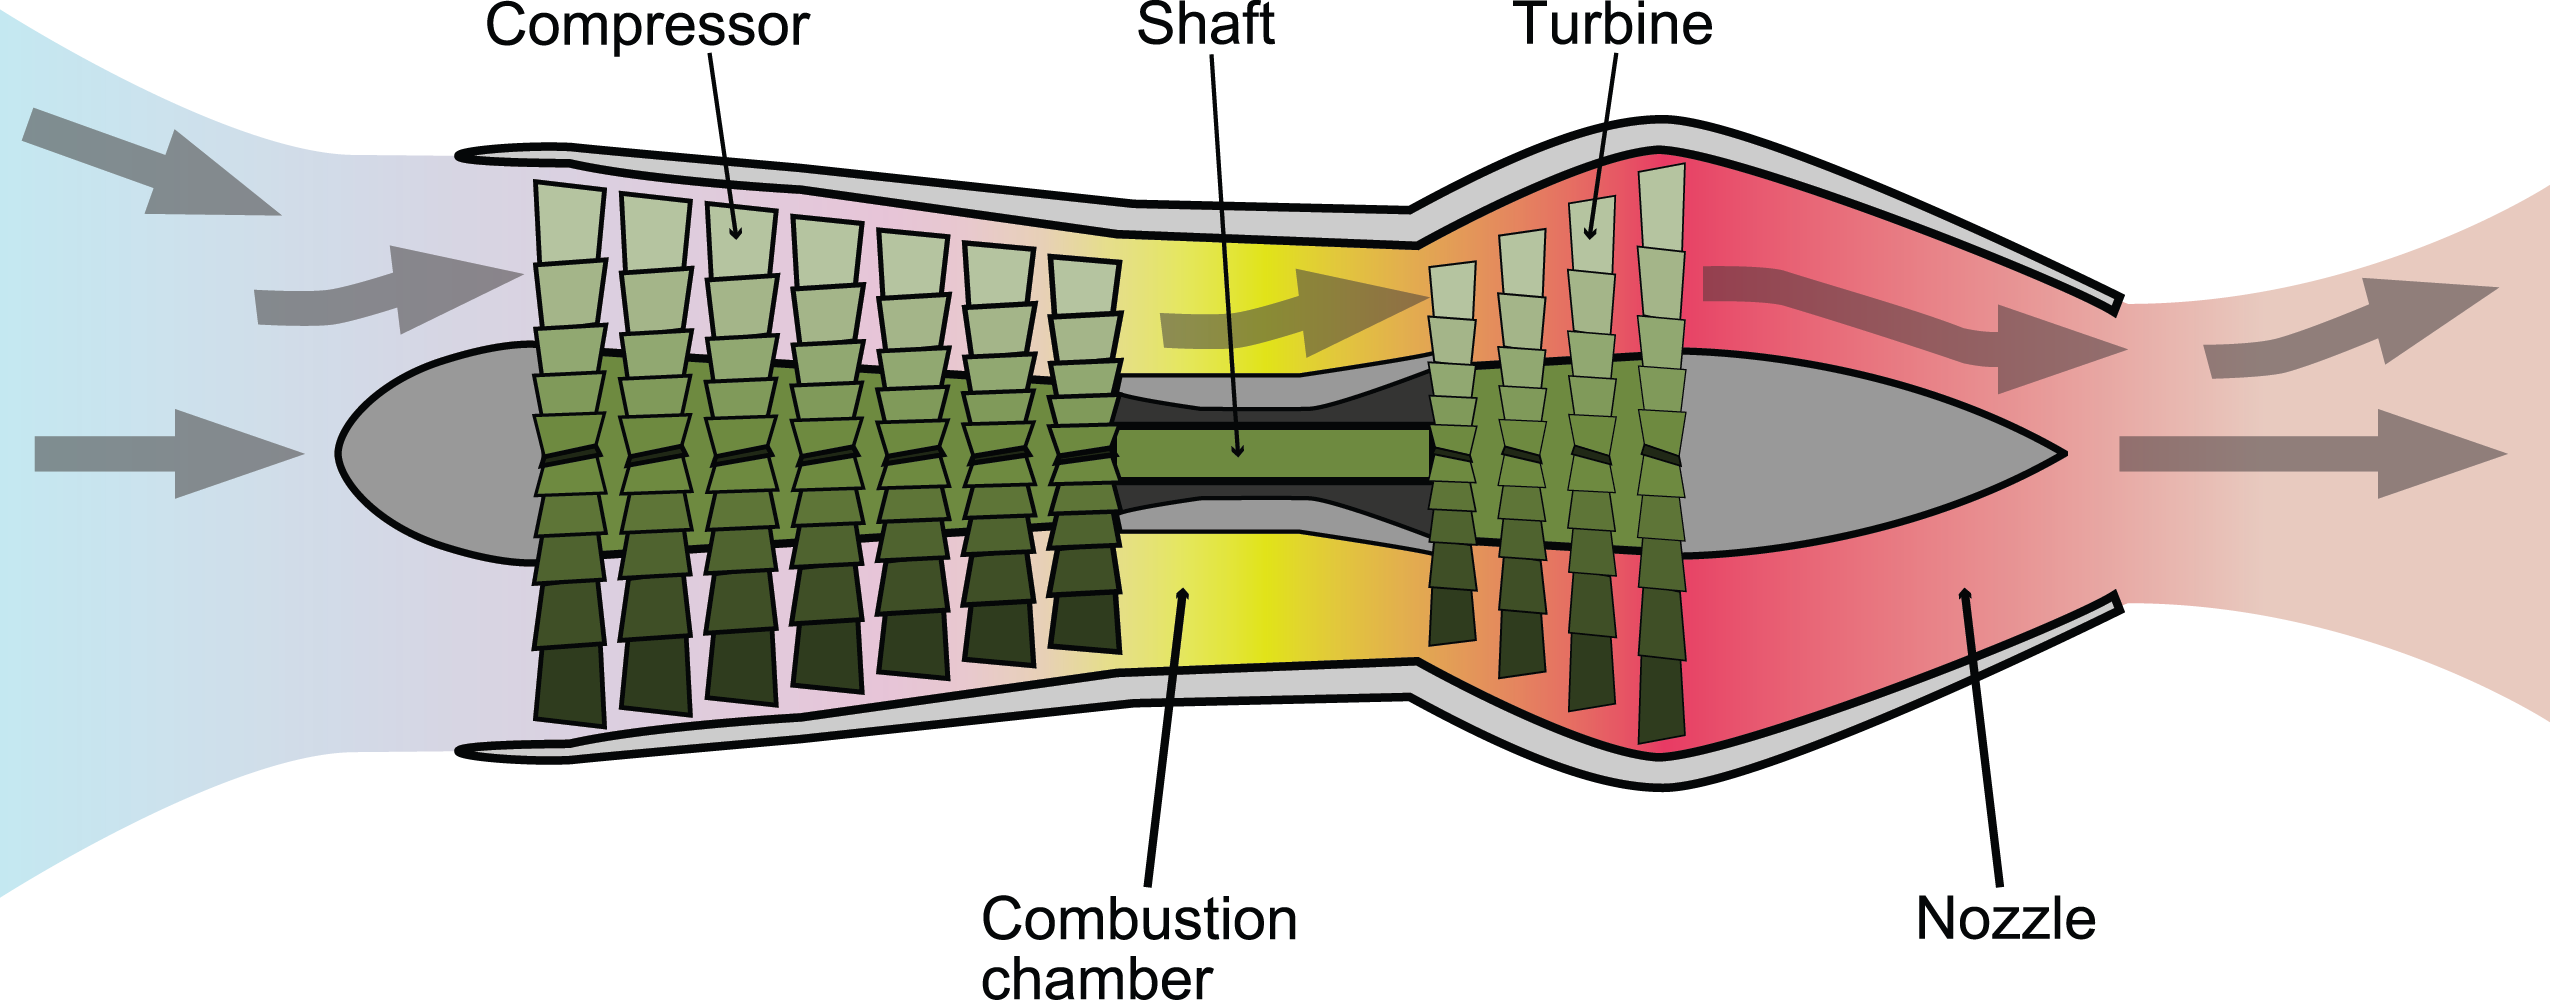
\includegraphics[width=.7\linewidth]{turbojetDiagram}
  \caption{A diagram showing the various components of a turbojet engine. Credit: EmoScopes, \href{https://commons.wikimedia.org/wiki/File:Turbojet_operation-axial_flow-en.svg}{Wikipedia}.}
  \label{fig:turbojet}
\end{figure}

\subsubsection*{Kinetic Energy in the Diffuser and Nozzle}

There are some concepts here that we have not thoroughly covered.  For instance, the diffuser and nozzle are the first components for which the velocity of the fluid is important. Everywhere else in the engine and the book, we assume that kinetic energy is negligble, but we cannot ignore it in these two components.  In other words, we will not neglect the kinetic energies of states 1 and 6, which will be represented as $KE_1$ and $KE_6$ (extensive properties) or $ke_1$ and $ke_6$ (intensive properties).  However, the kinetic energies of all remaining states will be assumed to be negligible.

\subsubsection*{The Standard Atmosphere}
Second, jet engines only operate at ground level for a very short time in any given flight.  Most of the time is spent at altitude, which does not have the standard pressure and temperature.  To accurately choose values for state 1, we need to look at the {\bf standard atmosphere}, which is simple a list of pressures and temperatures at various altitudes.  Values from the International Standard Atmosphere are given in Appendix \ref{app:ISA}.

\subsubsection*{Thrust and Efficiency}
Finally, the purpose of jet engines is to provide {\bf thrust}.  The thrust can be calculated through the conservation of momentum.  The air moving through the engine requires a force to accelerate it from its inlet velocity to its exit velocity.  An equal and opposite force will act on the aircraft.  Since the air is accelerated toward the rear of the engine, the reaction force will propel the aircraft forward.

\begin{equation}\label{eq:thrust}
  \vec{T} = \dot{m} \left(\vec{V}_{out} - \vec{V}_{in}\right)
\end{equation}

In order to calculate the efficiency of a jet engine, we need to somehow compare the thrust to the heat provided through combustion of the fuel.  To do this, we define the {\bf propulsive power} as the dot product of the thrust $T$ and the velocity of the aircraft $\vec{V}_{\infty}$.
\begin{align}
  \nonumber \dot{W}_{prop} &= \vec{T} \cdot \vec{V}_{\infty} = \dot{m} \vec{V}_{\infty}\cdot\left(\vec{V}_{out} - \vec{V}_{in}\right)\\
  \label{eq:propulsivePower} w_{prop} &= \vec{V}_{\infty} \cdot \left(\vec{V}_{out} - \vec{V}_{in}\right)
\end{align}

As always, the efficiency of the engine is what we get out (propulsive power) divided by what we pay for it (heat from combustion), as shown in Equation \ref{eq:aircraftEfficiency}.

\begin{equation}\label{eq:aircraftEfficiency}
  \eta_{jet} = \frac{w_{prop}}{q_{comb}} = \frac{\vec{V}_{\infty} \cdot \left(\vec{V}_{out} - \vec{V}_{in}\right)}{h_4-h_3}
\end{equation}

Note that the efficiency is dependent not only on the thermodynamics of the cycle, but also the current speed of the aircraft.  For this reason, $\eta_{jet}$ is often called the {\bf overall efficiency}.  Often, the overall efficiency is broken into two parts, the {\bf propulsive efficiency} $\eta_{p}$ and the {\bf thermal efficiency}, $\eta_{th}$.

\begin{equation*}
  \eta_p = \frac{\vec{V}_{\infty} \cdot \left(\vec{V}_{out} - \vec{V}_{in}\right)}{h_6 - h_5} \qquad \qquad \eta_{th} = \frac{h_6 - h_5}{h_4 - h_3}
\end{equation*}

It can be seen that $\eta_p$ is the propulsive power divided by the excess enthalpy after the turbine, while $\eta_{th}$ is the excess enthalpy divided by the heat transfer in the combustion chamber.  Multiplying these two values together results in the overall efficiency.

\subsubsection{$h$-$s$ Diagram for a Turbojet}
Because air is superheated throughout the entire Brayton cycle, we can use the $h$-$s$ diagram of air to describe the turbojet, as shown in Figure \ref{fig:turbojet_hs}.

\begin{figure}[H]
  \centering
  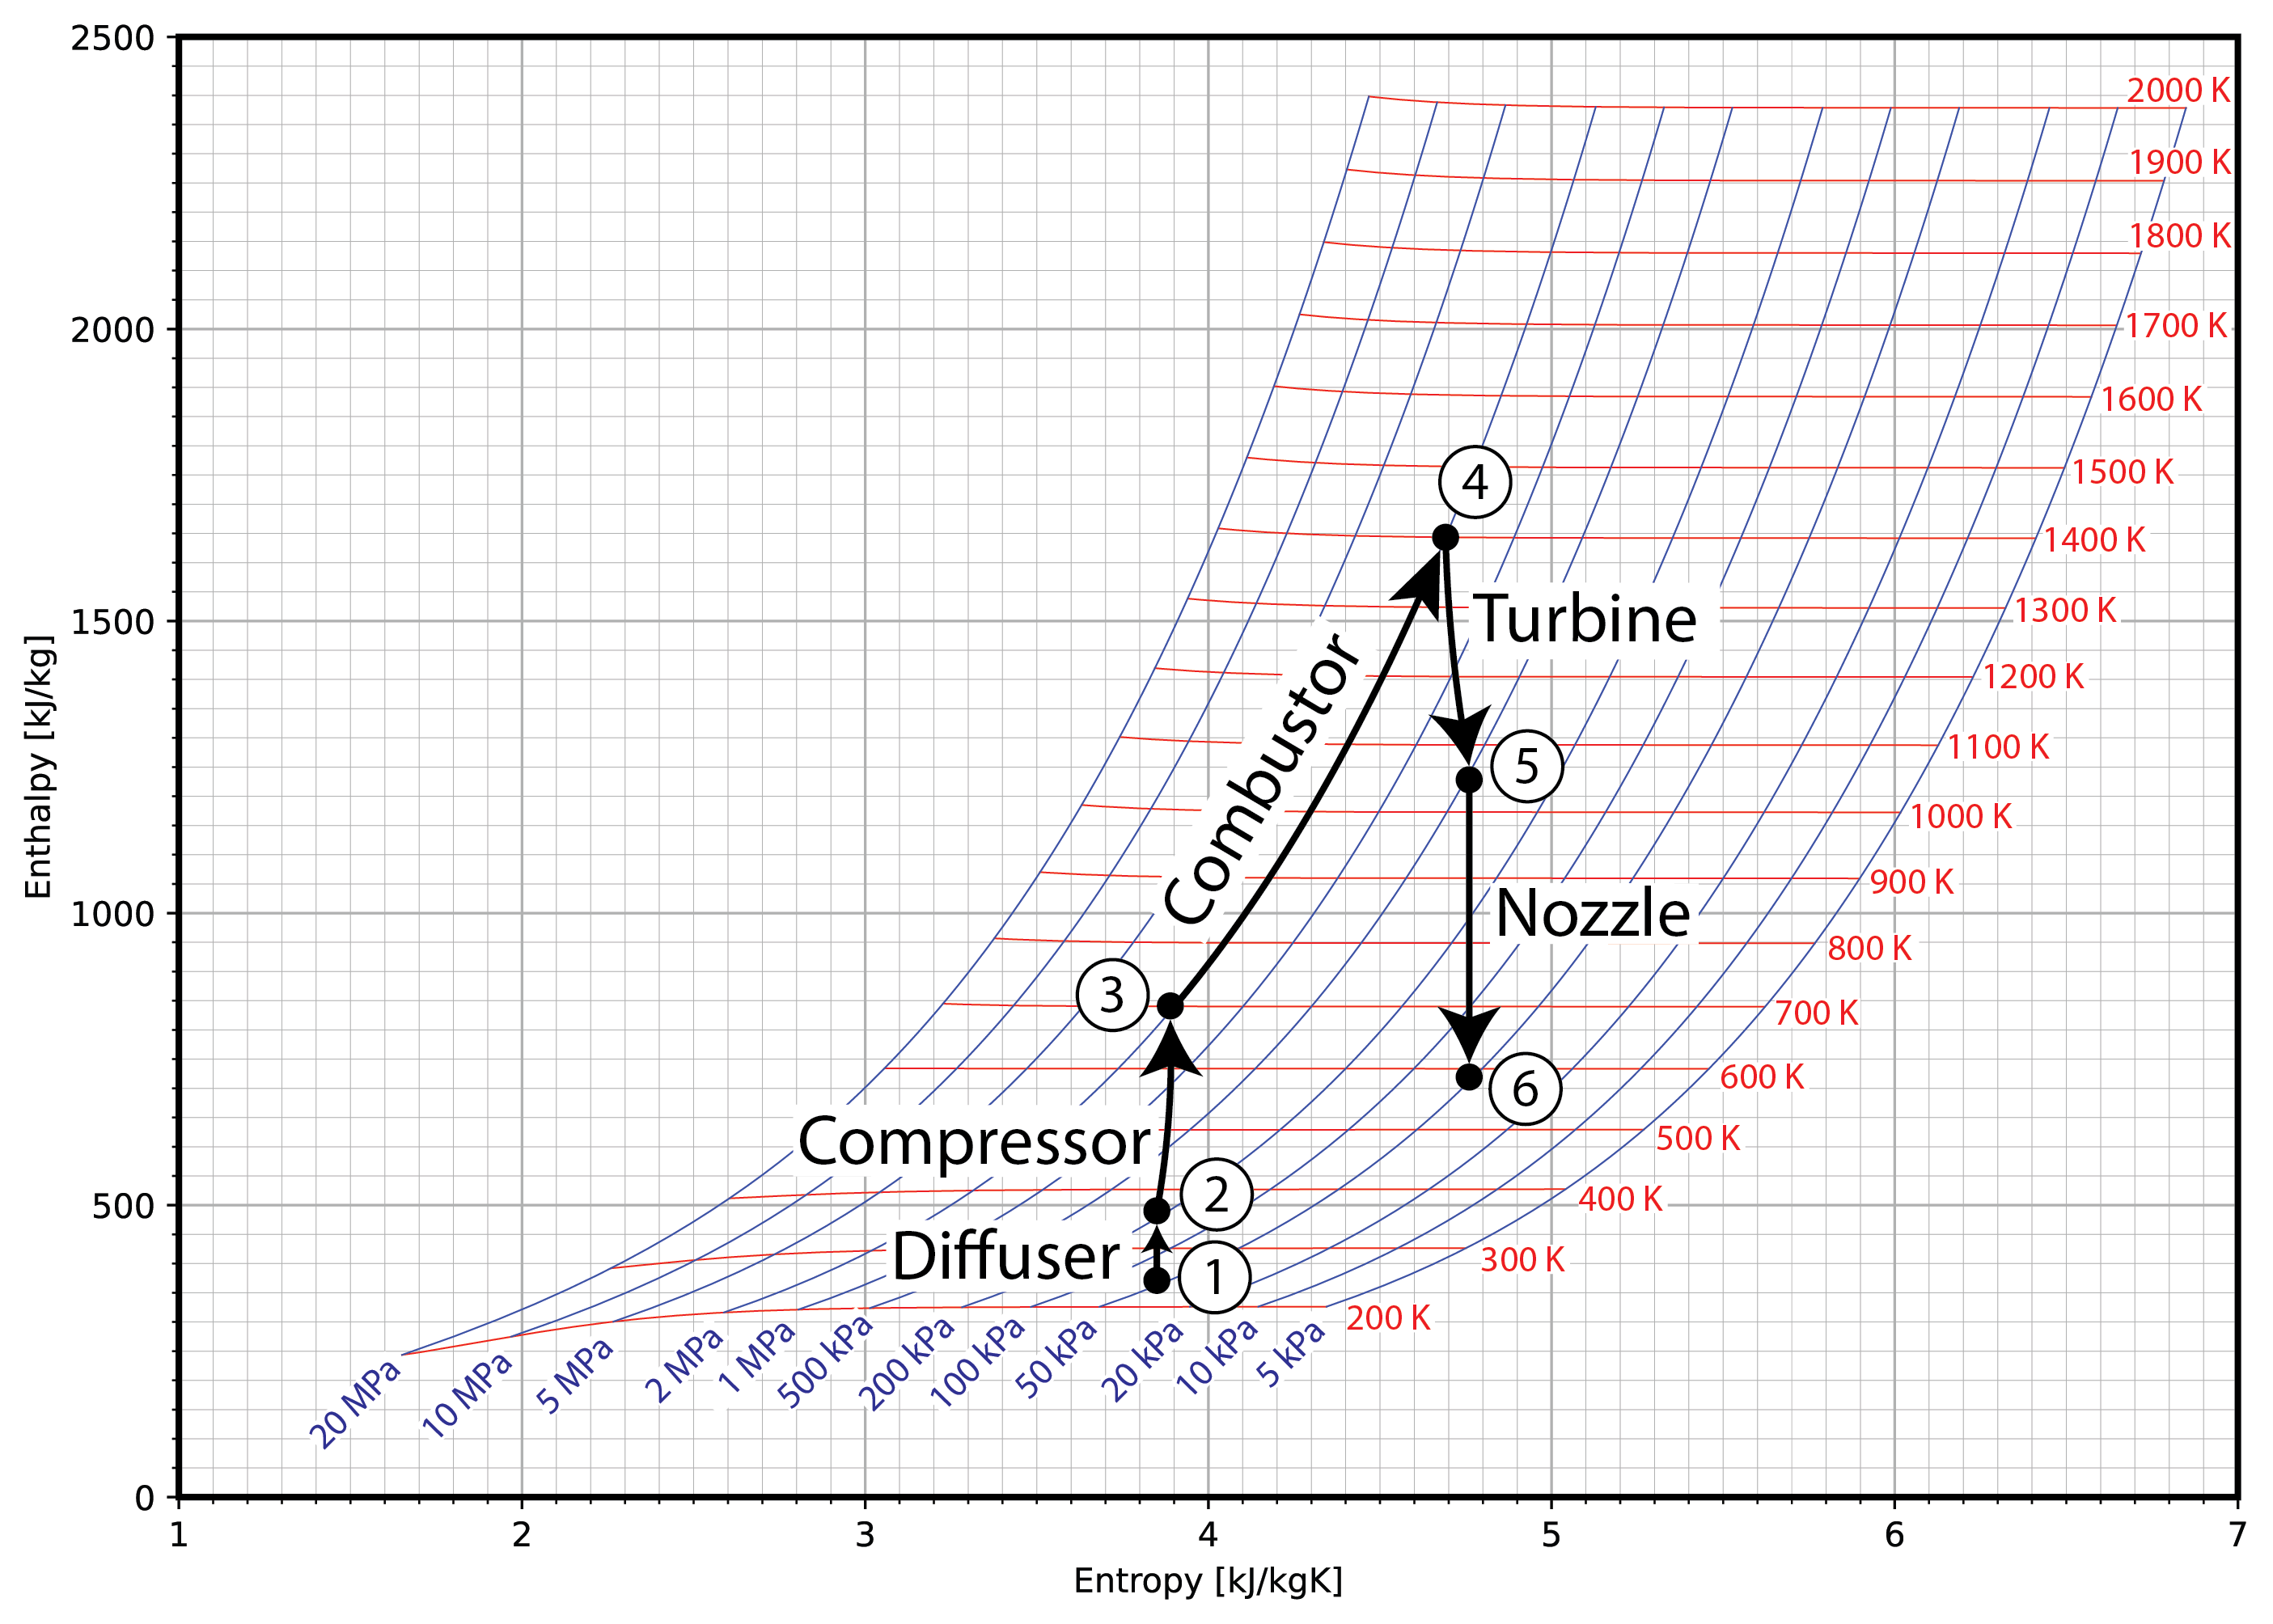
\includegraphics[width=.7\linewidth]{jetEnginehs}
  \caption{$h$-$s$ diagram of a turbojet.}
  \label{fig:turbojet_hs}
\end{figure}

Note that the diffuser and nozzle are assumed to be perfectly isentropic.  While there is typically a small increase in entropy through those components, we will neglect it in this book.  Example \ref{ex:turbojetIsentropic} will analyze a jet engine, assuming all components are isentropic. Example \ref{ex:turbojetReal} will analyze the same engine, but incorporating the isentropic efficiency of the compressor and turbine.

\begin{example}[label=ex:turbojetIsentropic]{Isentropic Analysis of a Turbojet}
  A turbojet is flying at a speed of 200 m/s at an altitude of 20 kilometers.  Assuming the pressure ratio of the compressor is 12 and the turbine inlet tempearture is 1250 K, determine the thrust provided by the engine, assuming the flow rate of air is 10 kg/s.

  \begin{enumerate}[a)]
  \item Determine the temperature, pressure, and enthalpy of each state.  Find the kinetic energy of appropriate states.
  \item Plot each state and process on the $h$-$s$ diagram for air.
  \item Find the work/heat transfer of each component.
  \item Determine the thrust and efficiency of the turbojet ($\eta_{jet}$)
  \end{enumerate}

  \subsubsection*{State 1 Properties}
  The pressure and temperature for state 1 can be determined directly from the standard atmosphere table in Appendix \ref{app:ISA}. Enthalpy and entropy can be found using CoolProp. 

  \begin{align*}
    p_1 &= 5.529 {\rm\, kPa} & T_1 &= 216.7 {\rm\, K} \\
    h_1 &= 342.9\, \frac{\rm kJ}{\rm kg} &  s_1 &= 4.396\, \frac{\rm kJ}{\rm kg\,K}
  \end{align*}
  
  Additionally, we can find the kinetic energy for state 1 from the velocity:
  \begin{equation*}
    ke_1 = \frac{1}{2} \left(200\, \frac{\rm m}{\rm s}\right)^2 = 10\, \frac{\rm kJ}{\rm kg}
  \end{equation*}

  \subsubsection*{State 2 Properties}
  Air flows through the diffuser to get to state 2.  We assume that the diffuser is isentropic, meaning that $s_2 = s_1$.  Additionally, the diffuser transfers the kinetic energy in state 1 to enthalpy.  Thus, the enthalpy for state 2 is found through:
  \begin{equation*}
    h_2 = h_1 + ke_1 = 342.9\, \frac{\rm kJ}{\rm kg} + 10\, \frac{\rm kJ}{\rm kg} = 352.9\, \frac{\rm kJ}{\rm kg}
  \end{equation*}
  
  With $h_2$ and $s_2$, we can determine the temperature and pressure of state 2 from CoolProp:
  \begin{align*}
    p_2 &= 7.520 {\rm\, kPa} & T_2 &= 236.7 {\rm\, K} 
  \end{align*}

  \subsubsection*{State 3 Properties}
  The compressor has a given pressure ratio, meaning that $p_3$ can be found through the definition of pressure ratio:
  \begin{equation*}
    p_3 = PR \cdot p_2 = 12 \cdot 7.520 {\rm\, kPa} = 90.24 {\rm\, kPa}
  \end{equation*}
  Additionally, we assume that the compressor is isentropic, so $s_3 = s_2$.  This gives us values of enthalpy and temperature from CoolProp:
  \begin{align*}
    h_3 &= 608.6\, \frac{\rm kJ}{\rm kg} &  T_3 &= 479.8 {\rm\, K}
  \end{align*}

  \subsubsection*{State 4 Properties}
  The combustor operates under constant pressure, so $p_4 = p_3$.  Additionally, we are given the turbine inlet temperature, which is $T_4 = 1500$ K.  Once again, we go to CoolProp to find enthalpy and entropy.
  \begin{align*}
    h_4 &= 1762.4 \frac{\rm kJ}{\rm kg} &  s_4 &= 5.664 \frac{\rm kJ}{\rm kg\,K}
  \end{align*}
  
  \subsubsection*{State 5 Properties}
  The turbine produces only enough power to run the compressor.  We can express this through the following equation:
  \begin{align*}
    w_{comp} &= w_{turb} \\
    h_3 - h_2 &= h_4 - h_5 \\
    h_5 = h_4 + h_2 - h_3 &= 1762.4\, \frac{\rm kJ}{\rm kg} + 352.9\, \frac{\rm kJ}{\rm kg} - 608.6\, \frac{\rm kJ}{\rm kg} = 1516.7\, \frac{\rm kJ}{\rm kg}
  \end{align*}
  Additionally, we assume that the turbine is isentropic, so $s_5 = s_4$.  CoolProp provides temperature and pressure.
  \begin{align*}
    p_5 &= 48.874 {\rm\, kPa} & T_5 &= 1295.2 {\rm\, K} 
  \end{align*}

  \subsubsection*{State 6 Properties}
  The pressure of state 6 will again be atmospheric ($p_6 = 5.529 {\rm\ kPa}$).  Assuming an isentropic nozzle ($s_6 = s_5$), this gives us enough to go to CoolProp for the final properties.
  \begin{align*}
    h_6 &= 890.8\, \frac{\rm kJ}{\rm kg} &  T_6 &= 747.3 {\rm\, K}
  \end{align*}

  Because the nozzle converts enthalpy to kinetic energy, we can calculate the kinetic energy of state 6:
  \begin{equation*}
    ke_6 = h_5 - h_6 = 1516.7\, \frac{\rm kJ}{\rm kg} - 890.8\, \frac{\rm kJ}{\rm kg} = 625.8\, \frac{\rm kJ}{\rm kg}
  \end{equation*}

  \subsubsection*{$h$-$s$ Diagram}
  With all of the properties in hand, we can plot each of the states on the $h$-$s$ diagram.
  \begin{center}
    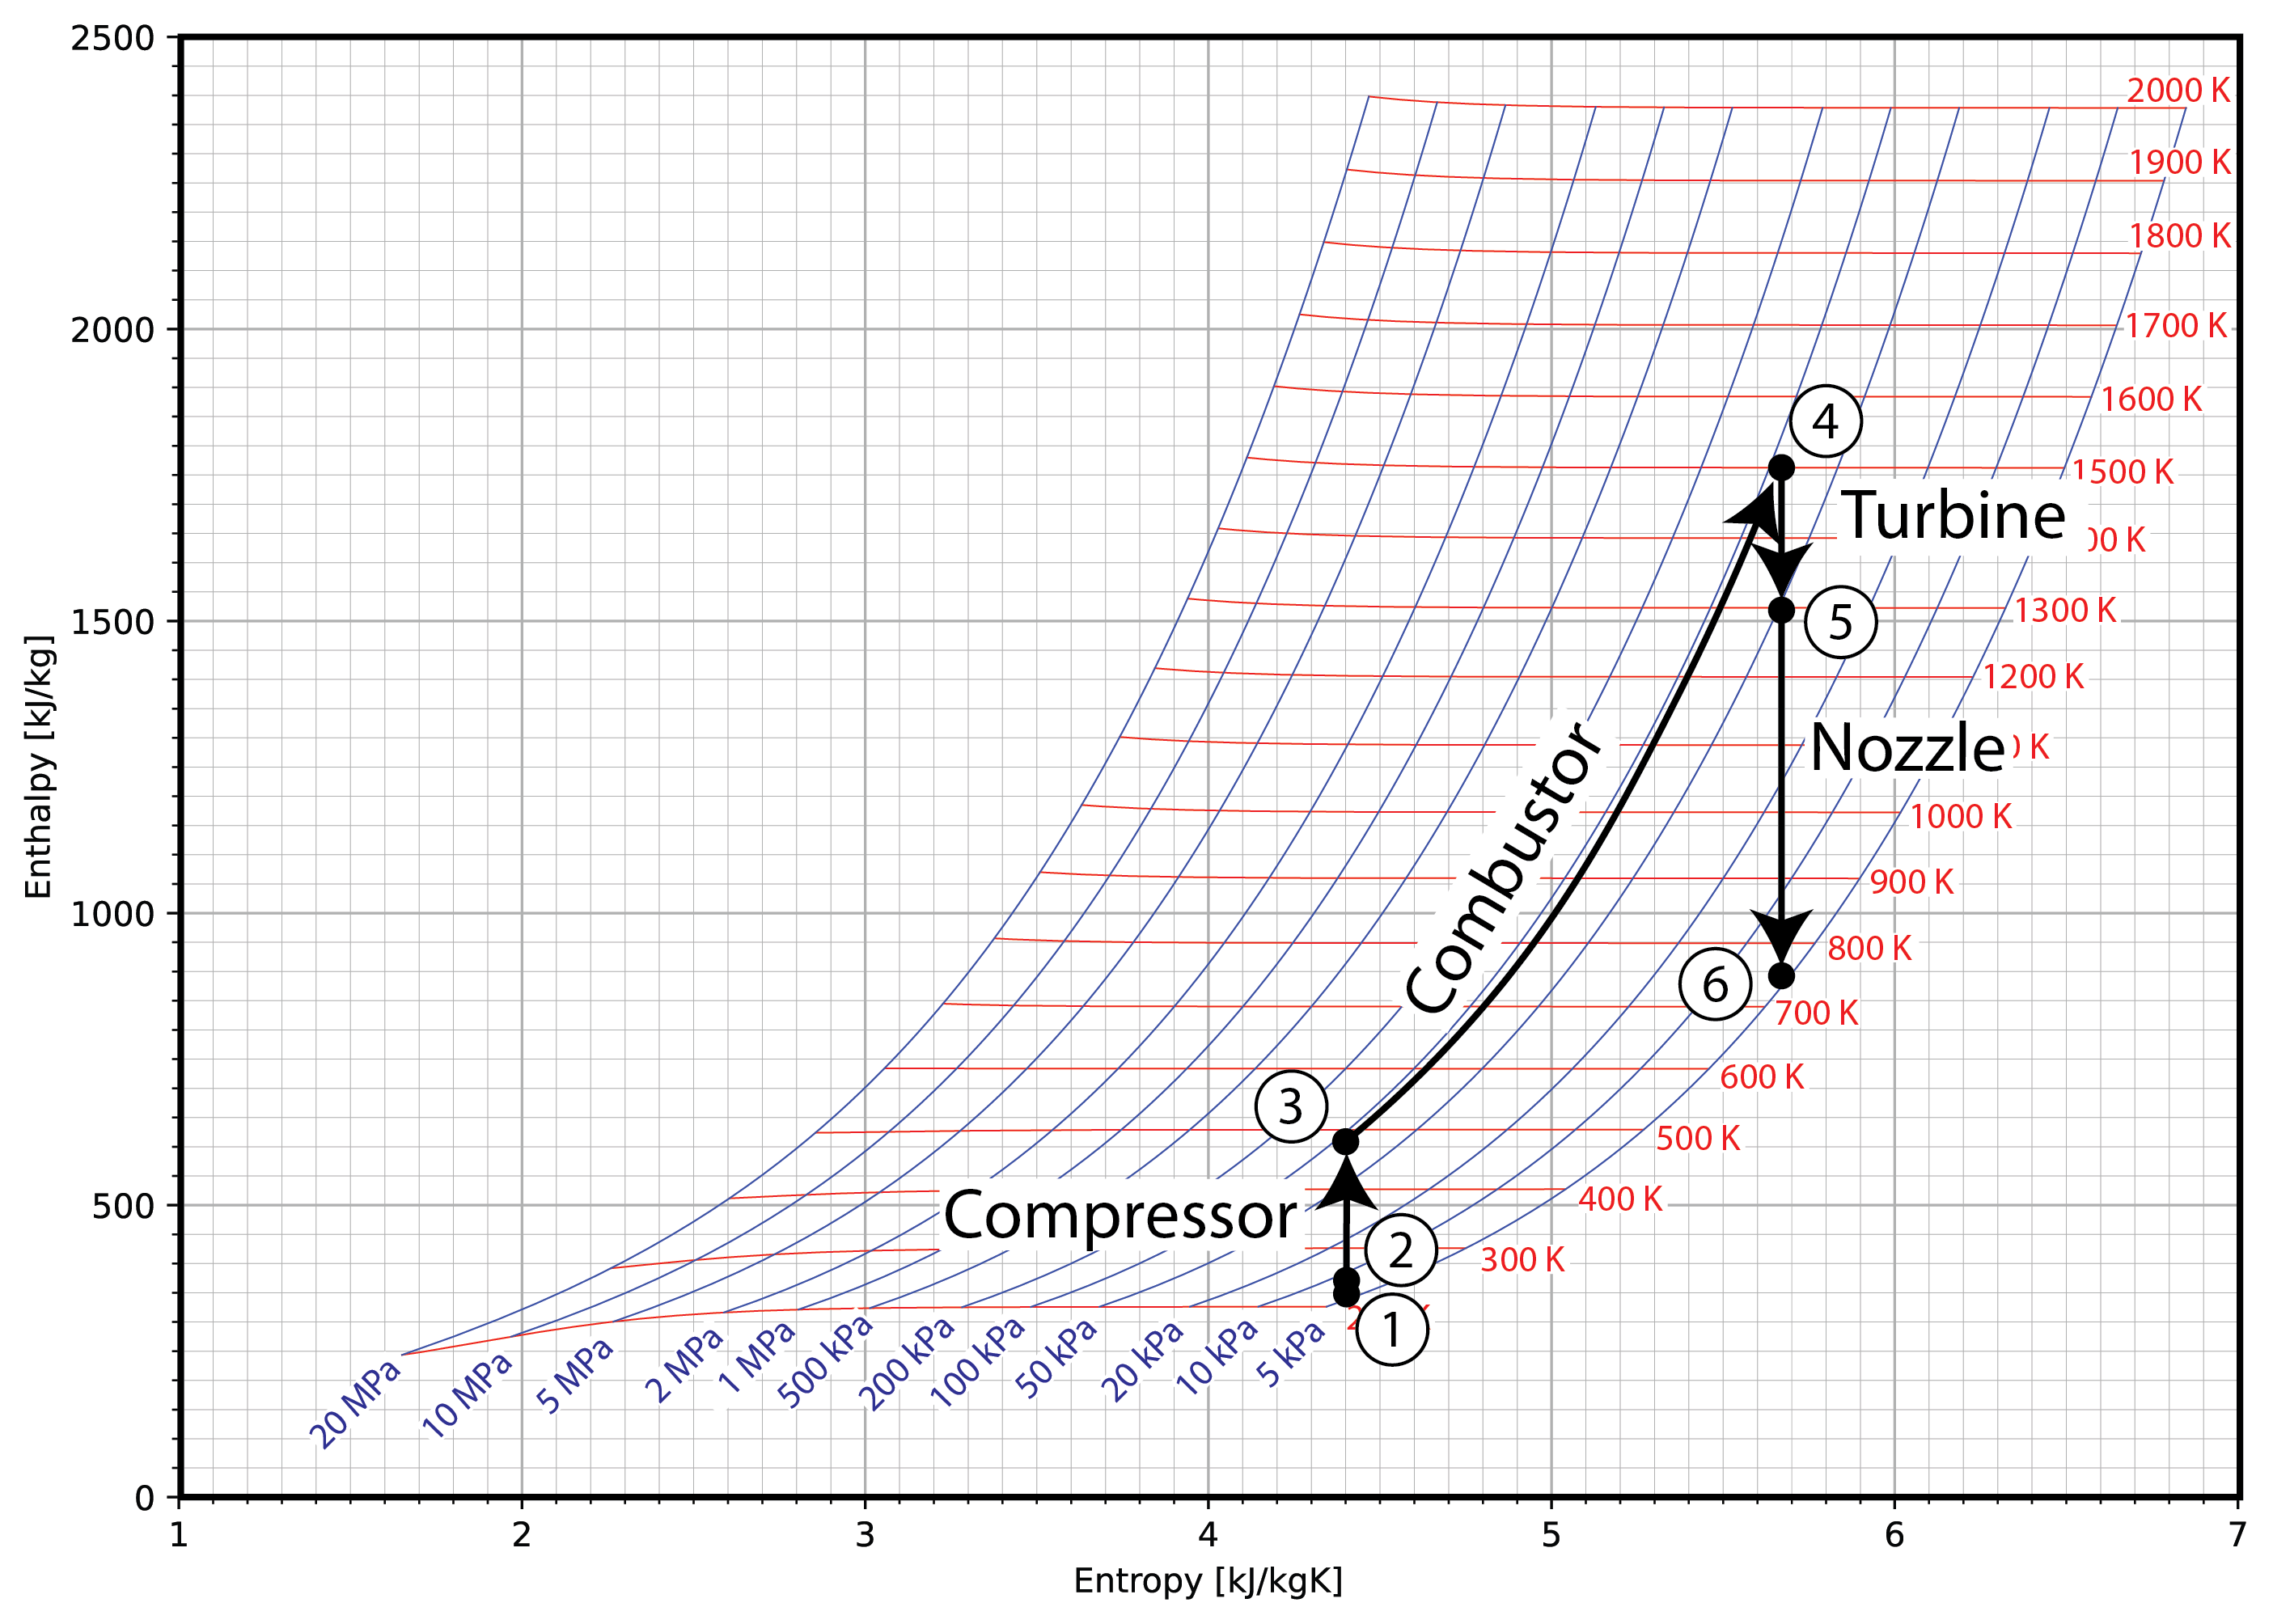
\includegraphics[width=0.75\linewidth]{isentropicTurbojetExample}
  \end{center}
  \subsubsection*{Component Analysis}
  The work for the compressor and turbine are equivalent:
  \begin{equation*}
    w_{comp} = w_{turb} = h_3 - h_2 = h_4 - h_5 = 245.7\, \frac{\rm kJ}{\rm kg}
  \end{equation*}

  The heat transfer from combustion is simply:
  \begin{equation*}
    q_{comb} = h_4 - h_3 = 1153.8\, \frac{\rm kJ}{\rm kg}
  \end{equation*}

  \subsubsection*{Thrust and Efficiency}
  In order to find thrust, we must first find the exit velocity.  This can be found from the kinetic energy at state 6:
  \begin{equation*}
    \vec{V}_6 = \sqrt{2 ke_6} = \sqrt{2 \left(625.8\, \frac{\rm kJ}{\rm kg}\right)} = 1118.7\, \frac{\rm m}{\rm s}
  \end{equation*}
  If the units feel weird above, keep in mind that a Joule can be broken down into $\rm N \cdot m$, which in turn becomes $\frac{\rm kg\, m}{\rm s^2} \cdot \rm m$.  Thus, a $\frac{\rm kJ}{\rm kg}$ is simply 1000 $\frac{\rm m^2}{\rm s^2}$.

  In any case, we can now calculate the thrust:
  \begin{equation*}
    \vec{T} = \dot{m} \left(\vec{V}_{out} - \vec{V}_{in}\right) = 10 \frac{\rm kg}{\rm s} \left(1118.7 \frac{\rm m}{\rm s} - 200 \frac{\rm m}{\rm s}\right) = \redbox{9187\, \rm N}
  \end{equation*}

  The propulsive power is:
  \begin{equation*}
    w_{prop} =  \left(\vec{V}_{out} - \vec{V}_{in}\right) \cdot \vec{V}_{\infty} = \left(1118.7\, \frac{\rm m}{\rm s} - 200\, \frac{\rm m}{\rm s}\right) \cdot 200\, \frac{\rm m}{\rm s} = 183.7\, \frac{\rm kJ}{\rm kg}
  \end{equation*}

  Finally, the turbojet efficiency is:
  \begin{equation*}
    \eta_{jet} = \frac{w_{prop}}{q_{comb}} = \frac{183.7\, \frac{\rm kJ}{\rm kg}}{1153.8\, \frac{\rm kJ}{\rm kg}} = \redbox{15.9\%}
  \end{equation*}
  This is a relatively low efficiency, which can be improved by:
  \begin{itemize}
  \item Reducing the exit velocity and increasing the flow rate, as is common in modern high-bypass turbofan engines
  \item Increasing the turbine inlet temperature, which can be accomplished through modern composite materials and active cooling (pumping coolant through microchannels in the turbine blades)
  \item Increasing the pressure ratio of the compressor
  \end{itemize}
\end{example}

% vvvvvvvvvvvvvvvvvvvvvvvvvvvvvvvvvvvvvvvvvvvvvvvvvvvvvvvvvvvvvvvvvvvv
\begin{example}[label=ex:turbojetReal]{Real Analysis of a Turbojet}

  The turbojet from Example \ref{ex:turbojetIsentropic} will again be analyzed, this time using an isentropic efficiency of 85\% for the compressor and an isentropic efficiency of 90\% for the turbine.

  A turbojet is flying at a speed of 200 m/s at an altitude of 20 kilometers.  Assuming the pressure ratio of the compressor is 12 and the turbine inlet tempearture is 1250 K, determine the thrust provided by the engine, assuming the flow rate of air is 10 kg/s.

  \begin{enumerate}[a)]
  \item Determine the temperature, pressure, and enthalpy of each state.  Find the kinetic energy of appropriate states.
  \item Plot each state and process on the $h$-$s$ diagram for air.
  \item Find the work/heat transfer of each component.
  \item Determine the thrust and efficiency of the turbojet ($\eta_{jet}$)
  \end{enumerate}

  \subsubsection*{Summary of Example \ref{ex:turbojetIsentropic}}
  The table below summarizes the results of the previous example.  Several states are no longer correct.  These states have been written in gray, while states that are still valid are in black.
  
  \begin{table}[H]
    \centering
    \def\arraystretch{1.5}
    %\caption{Tabular Representation of Energy Equation for Stirling Cycle}
    %\label{tab:ch3_stirling}
    \begin{tabular}{r|cccc}
      State & Pressure & Temperature & Enthalpy & Entropy \\ \hline
      1 & 5.53 kPa & 217 K & 342.9 $\frac{\rm kJ}{\rm kg}$ & 4.396 $\frac{\rm kJ}{\rm kg\,K}$ \\
      2 & 7.52 kPa & 237 K & 352.9 $\frac{\rm kJ}{\rm kg}$ & 4.396 $\frac{\rm kJ}{\rm kg\,K}$ \\
      3s & 90.2 kPa & 480 K & 608.6 $\frac{\rm kJ}{\rm kg}$ & 4.396 $\frac{\rm kJ}{\rm kg\,K}$ \\
      3 & 90.2 kPa & {\color{lightgray} 480 K} & {\color{lightgray} 608.6 $\frac{\rm kJ}{\rm kg}$} & {\color{lightgray}4.396 $\frac{\rm kJ}{\rm kg\,K}$} \\
      4 & 90.2 kPa & 1500 K & 1762.4 $\frac{\rm kJ}{\rm kg}$ & 5.664 $\frac{\rm kJ}{\rm kg\,K}$ \\
      {\color{lightgray} 5s} & {\color{lightgray} 48.874 kPa} & {\color{lightgray} 1295 K} & {\color{lightgray} 1516.7 $\frac{\rm kJ}{\rm kg}$} & {\color{lightgray} 5.664 $\frac{\rm kJ}{\rm kg\,K}$} \\
      {\color{lightgray} 5} & {\color{lightgray} 48.874 kPa} & {\color{lightgray} 1295 K} & {\color{lightgray} 1516.7 $\frac{\rm kJ}{\rm kg}$} & {\color{lightgray} 5.664 $\frac{\rm kJ}{\rm kg\,K}$} \\
      6 & 5.54 kPa & {\color{lightgray} 747 K} & {\color{lightgray} 890.8 $\frac{\rm kJ}{\rm kg}$} & {\color{lightgray} 5.664 $\frac{\rm kJ}{\rm kg\,K}$}
    \end{tabular}
    \def\arraystretch{1.0}
  \end{table}
  
  \subsubsection{State 3 Properties}
  In order to determine the properties after the real compressor, we need to follow the same process as in Example \ref{ex:isentropicEffCompressor}.  From the definition of the isentropic efficiency:
  \begin{align*}
    \eta_C &= \frac{w_s}{w_a} = \frac{h_{3s}-h_2}{h_3-h_2} \qquad \rightarrow \qquad h_{3} = \frac{1}{\eta_C} \left(h_{3s} -h_2\right) + h_2 \\
    h_{3} &= \frac{1}{0.85} \left(608.6 \frac{\rm kJ}{\rm kg} - 352.9 \frac{\rm kJ}{\rm kg} \right) + 352.9 \frac{\rm kJ}{\rm kg} = 652.0 \frac{\rm kJ}{\rm kg}
  \end{align*}

  Using the pressure and enthalpy of the new state 3, we can determine the entropy and temperature:
  
  \begin{align*}
    s_3 &= 4.482 \frac{\rm kJ}{\rm kg\, K} &  T_3 &= 521.9 {\rm K}
  \end{align*}

  As a result, the combustor now supplies slightly less heat:
  \begin{equation*}
    q_{comb} = h_4-h_3 = 1762.4 \frac{\rm kJ}{\rm kg} - 652.0 \frac{\rm kJ}{\rm kg} = 1110.4 \frac{\rm kJ}{\rm kg}
  \end{equation*}
  
  \subsubsection*{State 5s/5 Properties}
  At first glance, we do not have enough information to find all the properties for either state 5 or state 5s.  The entropy of state 5s will be the same as state 4 ($s_{5s}=s_4$), and the work of the real turbine must match the work of the real compressor ($h_3-h_2 = h_4-h_5$).  Thus, we have two separate states for which we know only one property, though we can say that:
  \begin{align*}
    s_{5s} &= 5.664 \frac{\rm kJ}{\rm kg\, K} &  h_5 &= 1473.3 \frac{\rm kJ}{\rm kg}
  \end{align*}
  
  Fortunately, states 5 and 5s are linked by the pressure ($p_5=p_{5s}$) and by the isentropic efficiency of the turbine ($\eta_T$).  These two additional constraints give us enough information to determine both states.

  We start with the definition of the isentropic efficiency:
  \begin{align*}
    \eta_T &= \frac{w_a}{w_s} = \frac{h_4-h_5}{h_4-h_{5s}} \qquad \rightarrow \qquad h_{5s} = \frac{1}{\eta_T} \left(h_5 -h_4\right) + h_4 \\
    h_{5s} &= \frac{1}{0.9} \left(1473.3\, \frac{\rm kJ}{\rm kg} -1762.4\, \frac{\rm kJ}{\rm kg}\right) + 1762.4\, \frac{\rm kJ}{\rm kg} = 1441.2\, \frac{\rm kJ}{\rm kg}
  \end{align*}

  Using CoolProp:
  \begin{align*}
    p_{5s} &= 39.690 {\rm\, kPa} & T_{5s} &= 1231.5 {\rm\, K} 
  \end{align*}

  Finally, we can use CoolProp with $p_5 = 39.69$ kPa and $h_5 = 1473.3\, \frac{\rm kJ}{\rm kg}$:
  \begin{align*}
    s_5 &= 5.690\, \frac{\rm kJ}{\rm kg\, K} &  T_5 &= 1258.7\, {\rm K}
  \end{align*}

  \subsubsection*{State 6 Properties}
  Finally, state 6 can be found assuming an isentropic nozzle ($s_6=s_5$), with the final pressure equivalent to atmospheric ($p_6=p_1$).  This is enough to use in CoolProp to find the enthalpy and temperature.
  
  \begin{align*}
    h_6 &= 910.3\, \frac{\rm kJ}{\rm kg} &  T_6 &= 765.3 {\rm\, K}
  \end{align*}

  \subsection*{$h$-$s$ Diagram}
  With all of the states updated, we can create an updated $h$-$s$ diagram for the engine.
  \begin{center}
    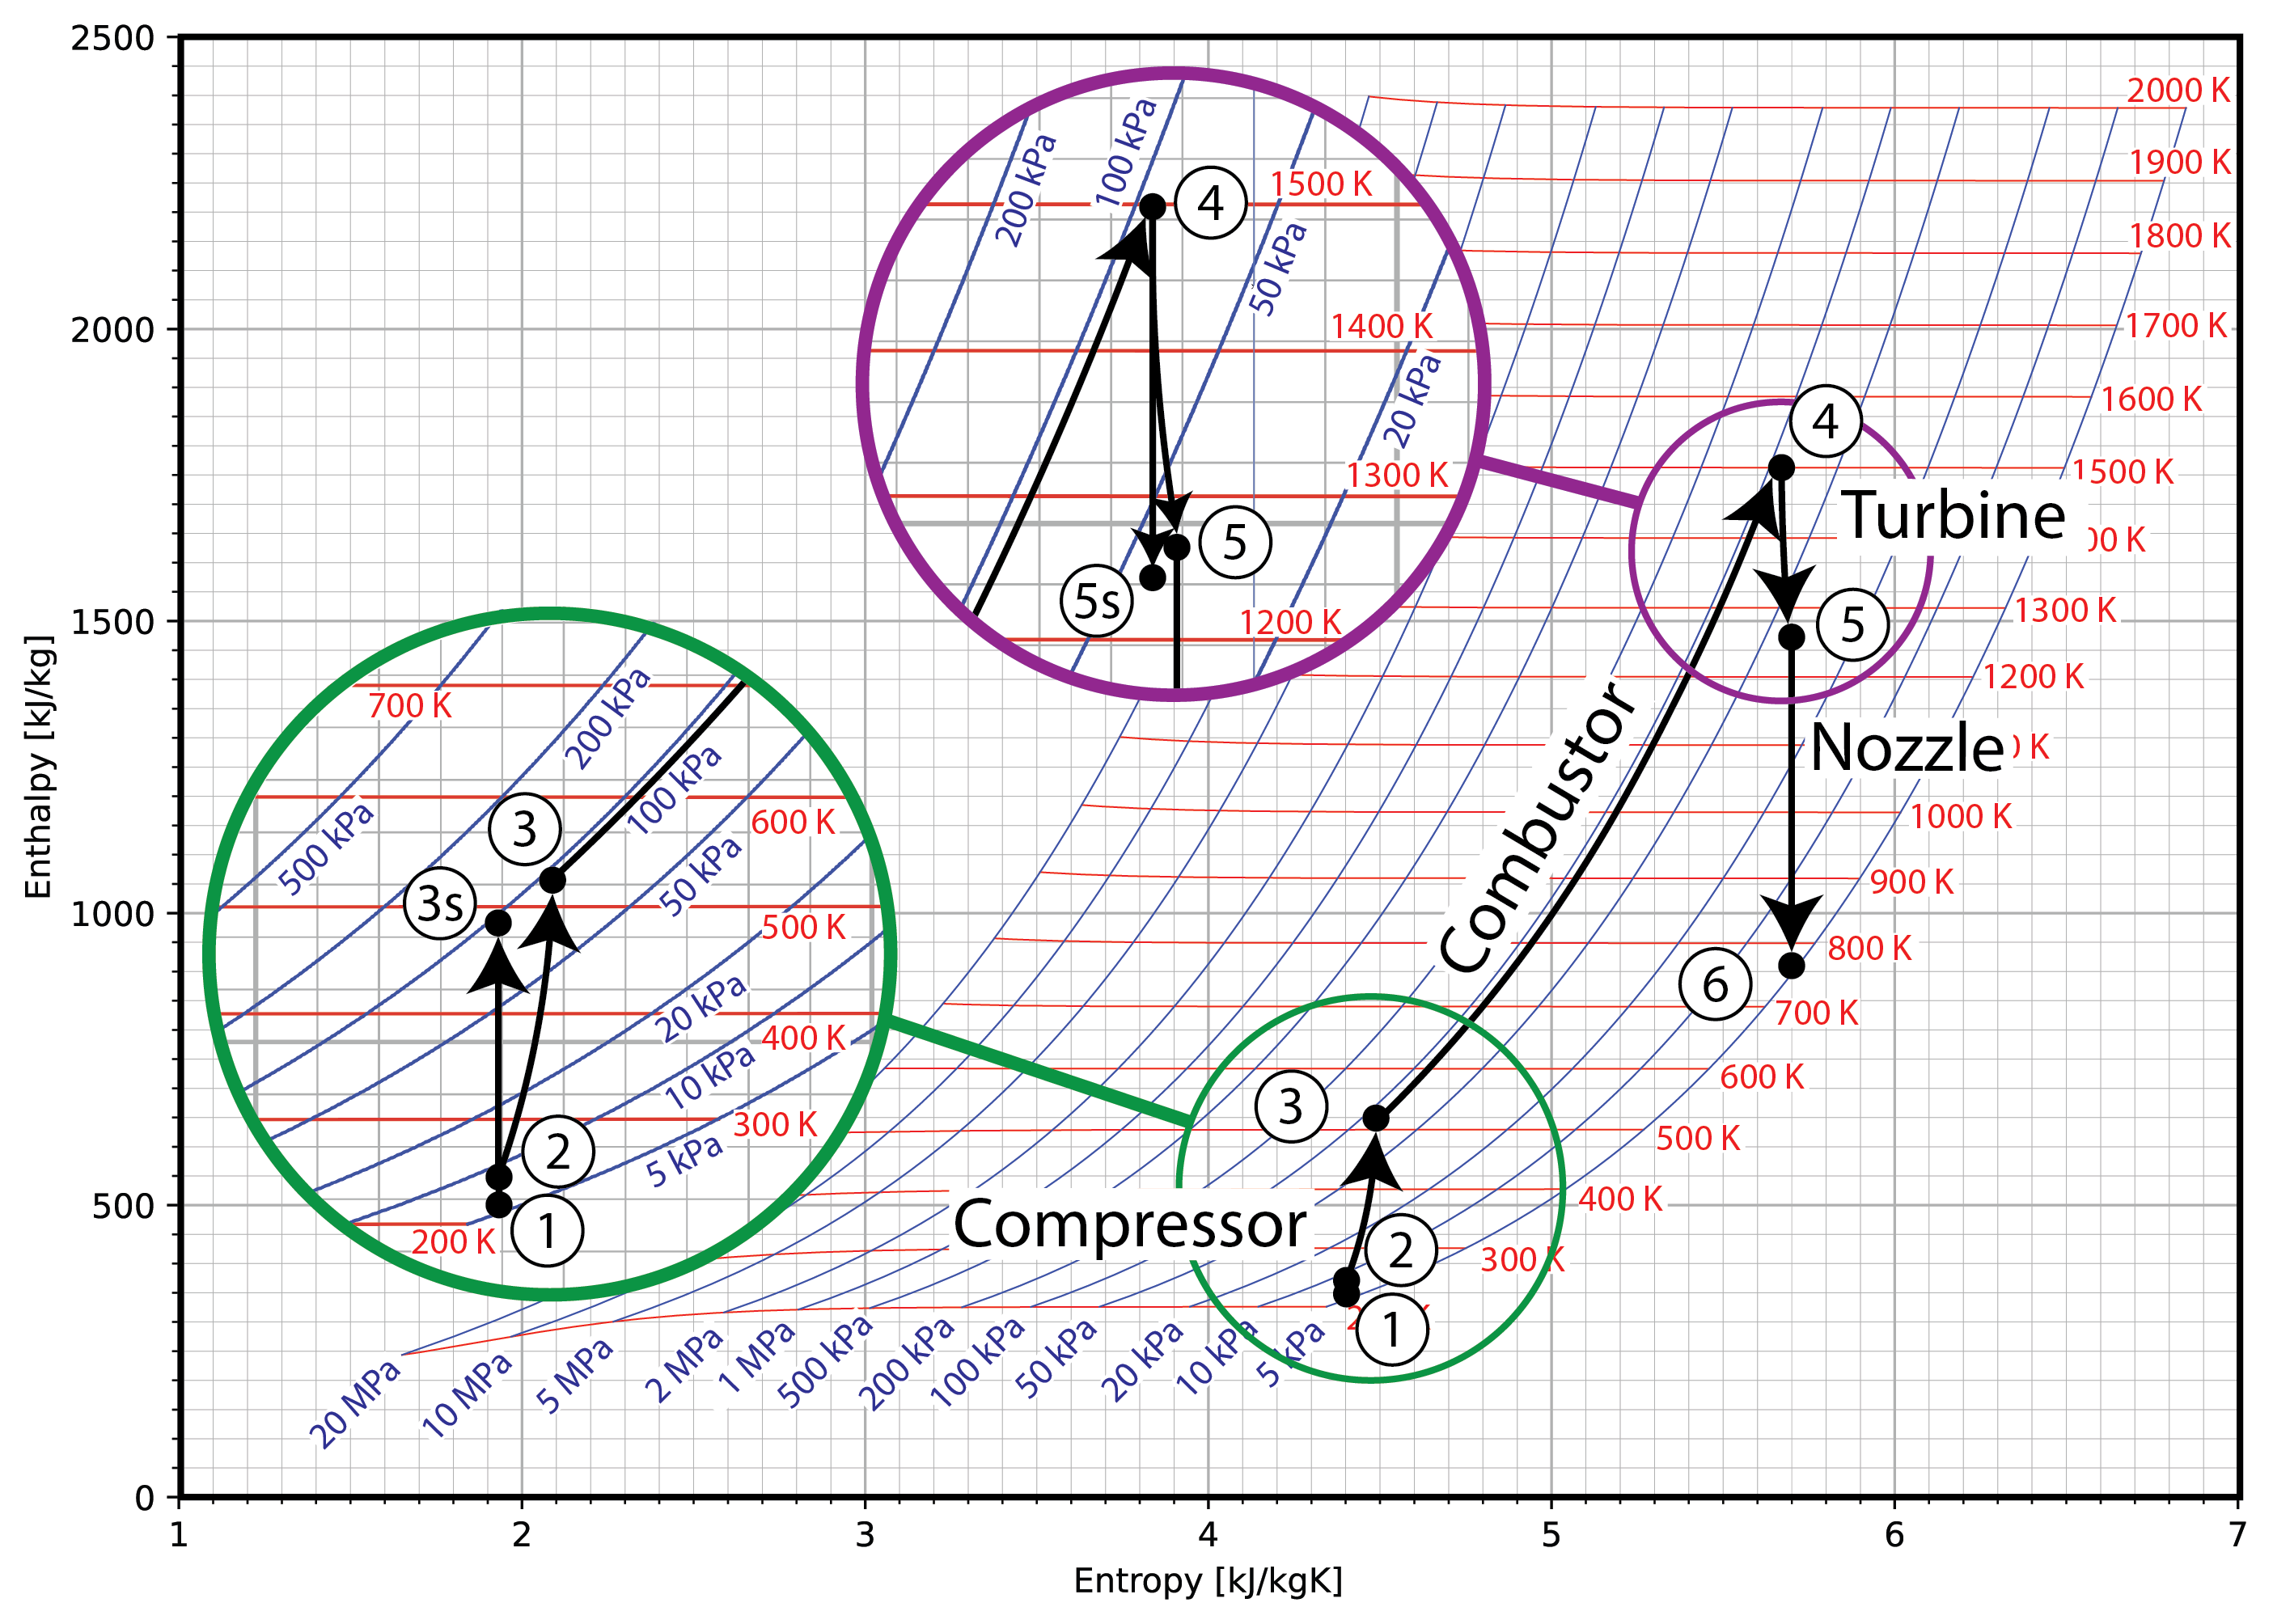
\includegraphics[width=0.75\linewidth]{realTurbojetExample}
  \end{center}
  
  
  \subsubsection*{Thrust and Efficiency}
  As in Example \ref{ex:turbojetIsentropic}, we find the kinetic energy at state 6, then use that to find the velocity.
  \begin{align*}
    ke_6 & = h_5 - h_6 = 1473.3\, \frac{\rm kJ}{\rm kg} - 910.3\, \frac{\rm kJ}{\rm kg} = 563.0\, \frac{\rm kJ}{\rm kg} \\
    \vec{V}_6 &= \sqrt{2 ke_6} = \sqrt{2 \left(563.0 \frac{\rm kJ}{\rm kg}\right)} = 1061.1\, \frac{\rm m}{\rm s}
  \end{align*}

  We can now calculate the thrust:
  \begin{equation*}
    \vec{T} = \dot{m} \left(\vec{V}_{out} - \vec{V}_{in}\right) = 10\, \frac{\rm kg}{\rm s} \left(1061.1\, \frac{\rm m}{\rm s} - 200\, \frac{\rm m}{\rm s}\right) = \redbox{8611\, \rm N}
  \end{equation*}

  The propulsive power is:
  \begin{equation*}
    w_{prop} =  \left(\vec{V}_{out} - \vec{V}_{in}\right) \cdot \vec{V}_{\infty} = \left(1061.1\, \frac{\rm m}{\rm s} - 200\, \frac{\rm m}{\rm s}\right) \cdot 200 \, \frac{\rm m}{\rm s} = 172.2\, \frac{\rm kJ}{\rm kg}
  \end{equation*}

  Finally, the turbojet efficiency is:
  \begin{equation*}
    \eta_{jet} = \frac{w_{prop}}{q_{comb}} = \frac{172.2 \frac{\rm kJ}{\rm kg}}{1110.4 \frac{\rm kJ}{\rm kg}} = 0.155
  \end{equation*}

  Thus, the efficiency is reduced from 15.9\% to 15.5\% by accounting for the non-ideal compressor and turbine.
  
\end{example}
% vvvvvvvvvvvvvvvvvvvvvvvvvvvvvvvvvvvvvvvvvvvvvvvvvvvvvvvvvvvvvvvvvvvv



\subsection{Turbofan Engine}
%--------------------------------------------------------------------
The turbofan adds the additional complication of splitting the gas flow, and introduces the concept of a {\bf bypass ratio} (BPR).
\begin{equation*}
  {\rm BPR} = \frac{\dot{m}_{bypass}}{\dot{m}_{comp}}
\end{equation*}

The various components of a turbofan can be seen in Figure \ref{fig:turbofan}.  Of note, the rotational speed of the fan is typically lower than what is required for the compressor, so there are typically two shafts (labelled low-pressure and high-pressure shafts).  For our analysis, we will neglect these details, and lump together the two compressors and the two turbines.

\begin{figure}[H]
  \centering
  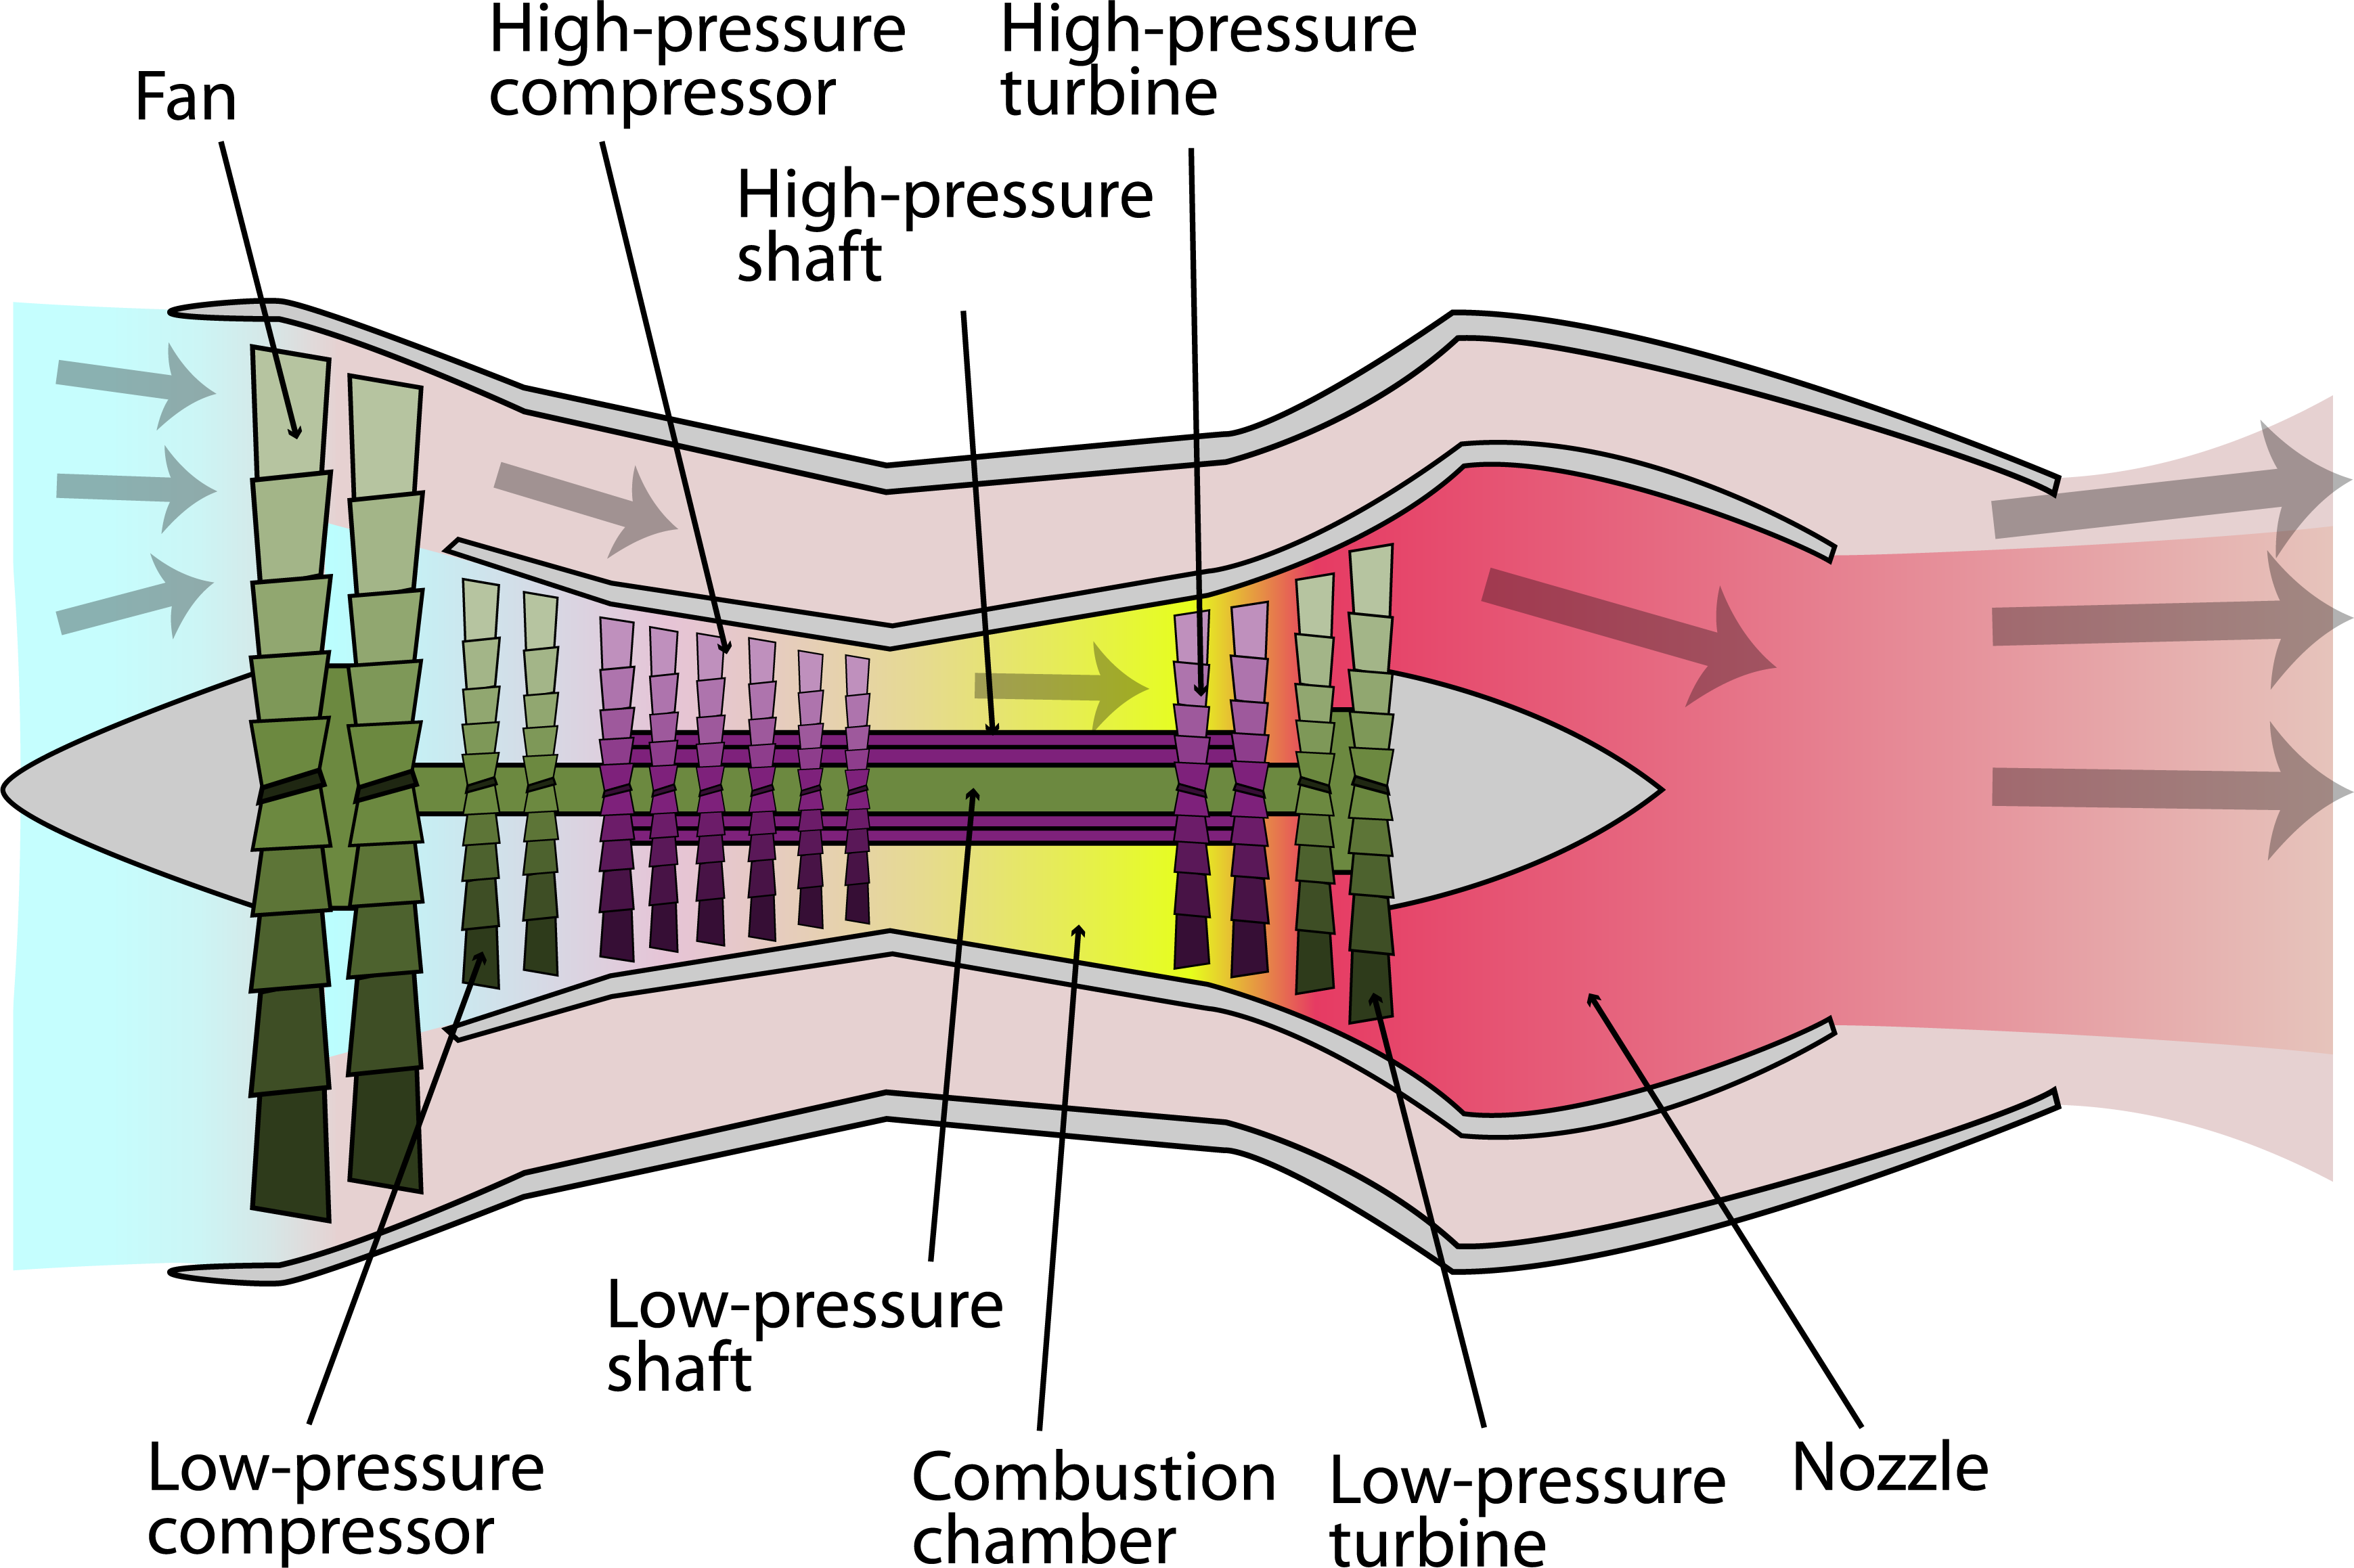
\includegraphics[width=.7\linewidth]{turbofanDiagram}
  \caption{A diagram showing the various components of a turbofan engine. Credit: K.Aainsqatsi, \href{https://commons.wikimedia.org/wiki/File:Turbofan_operation_lbp.svg}{Wikipedia}.}
  \label{fig:turbofan}
\end{figure}



\subsection{Turboprop/Helicopter Gas Turbine Engine}
%--------------------------------------------------------------------
The gas turbine engine for usage in turboprops is shown below:

\begin{figure}[H]
  \centering
  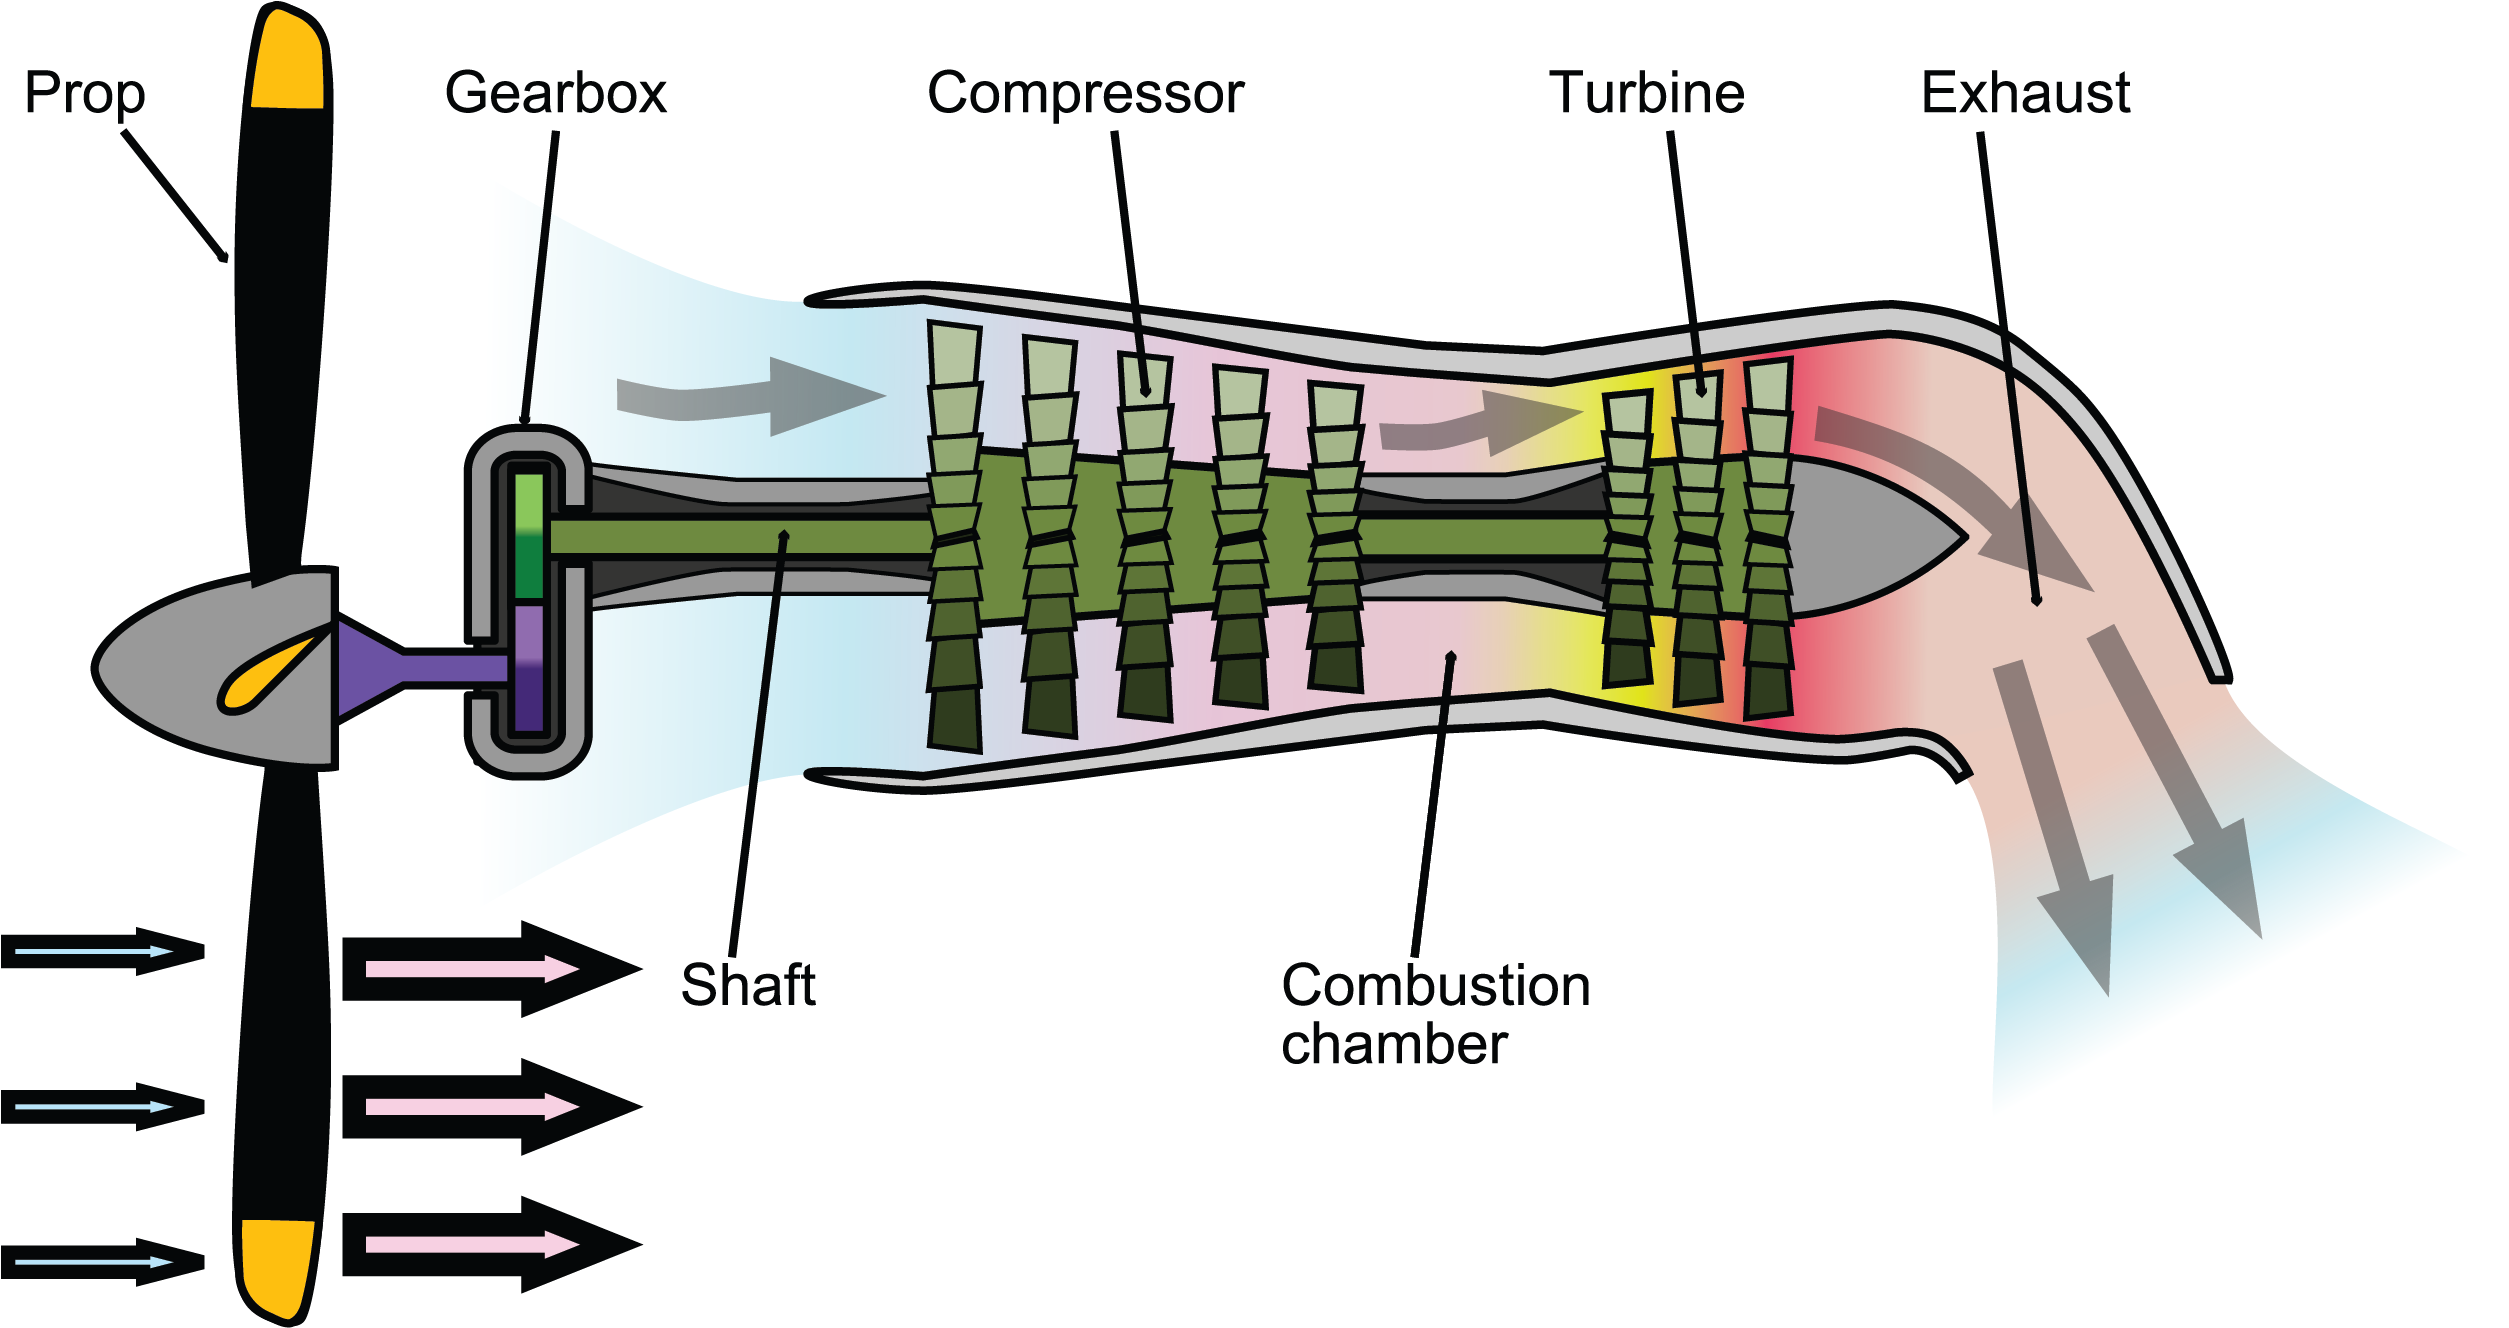
\includegraphics[width=.7\linewidth]{turbopropDiagram}
  \caption{A diagram showing the various components of a turbofan engine. Credit: Emoscopes, \href{https://commons.wikimedia.org/wiki/File:Turboprop_operation-en.svg}{Wikipedia}.}
  \label{fig:turboprop}
\end{figure}

In this case we see that there is no diffuser or nozzle, and that the turbine section has been replaced by two independent turbines - a "gas generator", or "gassifier" turbine to drive the compressor, and an output turbine to drive the helicopter blades. A typical gas turbine engine of this type is the General Electric T700 engine shown below, which is used in the Army Black Hawk helicopter.

\begin{figure}[H]
\centering
\begin{subfigure}{.5\textwidth}
  \centering
  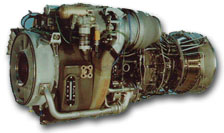
\includegraphics[width=.8\linewidth]{t700_baseline}
  \caption{Photograph of the GE T700 engine.}
  \label{fig:t700_baseline}
\end{subfigure}%
\begin{subfigure}{.5\textwidth}
  \centering
  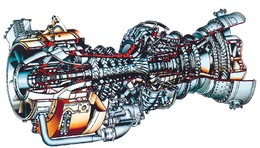
\includegraphics[width=.8\linewidth]{t700_section}
  \caption{Section view schematic of GE T700 engine.}
  \label{fig:t700_section}
\end{subfigure}
%\caption{}
%\label{fig:minimalHeatEnginePump}
\end{figure}

% vvvvvvvvvvvvvvvvvvvvvvvvvvvvvvvvvvvvvvvvvvvvvvvvvvvvvvvvvvvvvvvvvvvv
\begin{example}[label=ex:T700]{GE T700 Gas Turbine Engine}
  We wish to do an ideal thermodynamic analysis of the General Electric T700 gas turbine engine.
  \begin{center}
    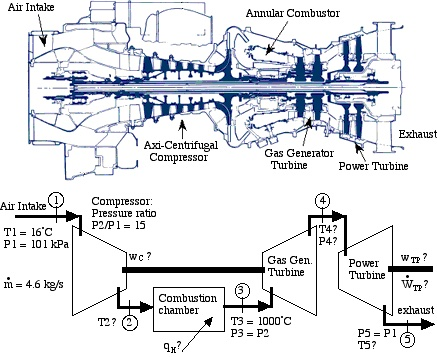
\includegraphics[width=.8\linewidth]{gas_turbine}
  \end{center}
  Notice that there are two turbines operating on independent output shafts. The High Pressure (first) turbine, named the Gas Generator Turbine, is directly connected by a shaft to the compressor. Its sole purpose is to drive the the axial/centrifugal compressor, thus the energy output of this turbine must equal the energy consumed by the compressor. The Low Pressure (second) turbine, named the Power Turbine, is connected via gearing to the helicopter rotor.

  {\bf Note:} Because of the large temperature variation throughout this problem we will need to consider the temperature dependence of the specific heat capacities of air. In the above schematic diagram we see that the temperature extremes of the system are 16°C - 1000°C (289 K - 1273 K), giving an average temperature of 781 K. From the table of Specific Heat Capacities of Air we see that at 800 K, $c_p$ = 1.099 [kJ/kgK] and the ratio of specific heat capacities $\gamma$ = 1.354, thus we use those values throughout this problem.
  
  Assume that the compressor and both turbines are isentropic, and that the combustion process occurs at constant pressure (isobaric). Using the information shown on the schematic diagram above, do the following:
  \begin{enumerate}[a)]
  \item  Sketch the entire process on an $h$-$s$ diagram, clearly showing the 5 stations on the diagram and the relevant isentropic and constant pressure lines.
  \item Determine the energy consumed by the compressor \answer{[$w_C$ = -328 kJ/kg]}, and the temperature at the outlet of the compressor \answer{[$T_2$ = 587 K]}.
  \item Determine the heat energy absorbed by the working gas in the combustion chamber \answer{[$q_H$ = 754 kJ/kg]}.
  \item Determine the temperature \answer{[$T_4$ = 975 K]} and the pressure \answer{[$p_4$ = 546 kPa]} at the outlet of the gas generator turbine.
  \item Determine the temperature \answer{[$T_5$ = 627 K]} and energy output of the power turbine \answer{[$w_{PT}$ = 382.5 kJ/kg]}.
  \item Given that the mass flow rate of the working gas through the system is 4.6 kg/s, determine the power output of the power turbine \answer{[1.76 MW]}.
  \end{enumerate}

  {\bf Solution:}
  information shown on the schematic diagram above, do the following:
  \begin{enumerate}[a)]
  \item  Sketch the entire process on an $h$-$s$ diagram, clearly showing the 5 stations on the diagram and the relevant isentropic and constant pressure lines.

    Unlike the case with a pure fluid such as steam, the $h$-$s$ diagram is not drawn to scale. Instead, is sketched in order to provide an intuitive graphical understanding of the problem.

    Furthermore, for an ideal gas the enthalpy is proportional to the temperature, hence the y-axis can be considered either an enthalpy or temperature axis. The various temperatures and pressures shown on this diagram are evaluated and plotted as we progress with the solution.

  \begin{center}
    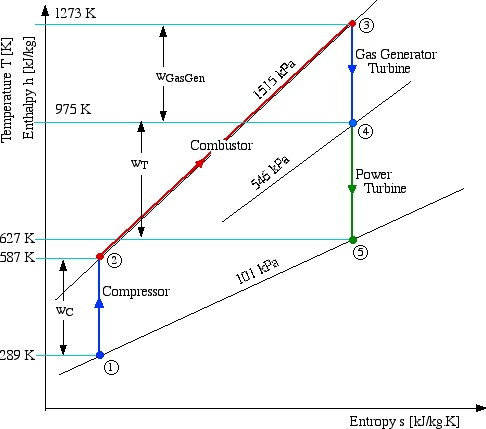
\includegraphics[width=.9\linewidth]{T700_h_s}
  \end{center}
      
   
\item Determine the energy consumed by the compressor, and the temperature at the outlet of the compressor.

  Ideally both the compressor and the turbine are isentropic devices, thus given the pressure ratio, in order to determine the temperature we consider the isentropic relations developed for an ideal gas.

  
  \begin{center}
    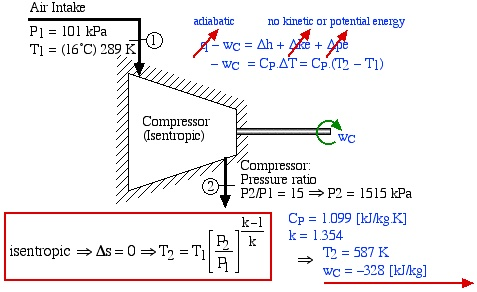
\includegraphics[width=.9\linewidth]{compressor}
  \end{center}
  
\item Determine the heat energy absorbed by the working gas in the combustion chamber.
  
  \begin{center}
    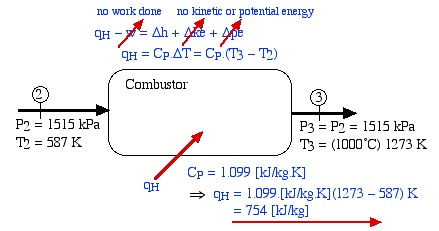
\includegraphics[width=.9\linewidth]{combustor}
  \end{center}
  
\item Determine the temperature and the pressure at the outlet of the gas generator turbine.

  Once more. since both turbines are isentropic, we use the pressure temperature relations developed for an isentropic process of an ideal gas.

  \begin{center}
    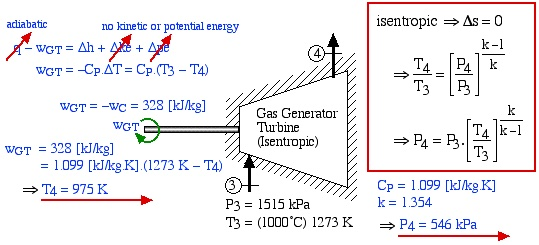
\includegraphics[width=.9\linewidth]{gasgen_turb}
  \end{center}
    
\item Determine the temperature and energy output of the power turbine.
  
  \begin{center}
    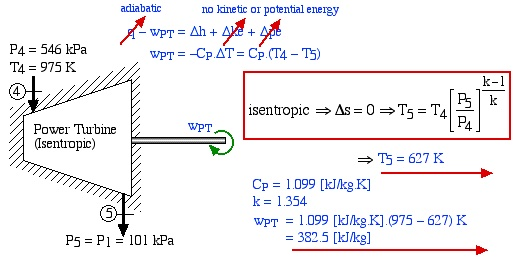
\includegraphics[width=.9\linewidth]{power_turb}
  \end{center}
\item Given that the mass flow rate of the working gas through the system is 4.6 kg/s, determine the power output of the power turbine.

  \begin{equation*}
    \dot{W}_{PT} = \dot{m} w_{PT} = 4.6 \frac{\rm kg}{\rm s} \cdot 382.5\frac{\rm kJ}{\rm kg} = 1.76\ {\rm MW}
  \end{equation*}
  \end{enumerate}

  Note that the actual power output of the T700 engine is around 1800 hp, which is significantly less than the above value ($\approx$ 2360 hp). This is because we have assumed that the compressor and both turbines are isentropic, which will never occur in practice. In a later problem, we will extend this exercise to consider a non-isentropic compressor and turbines.
\end{example}
% vvvvvvvvvvvvvvvvvvvvvvvvvvvvvvvvvvvvvvvvvvvvvvvvvvvvvvvvvvvvvvvvvvvv


\begin{homework}
  \question Consider the adiabatic steam turbine shown below.
  \begin{center}
    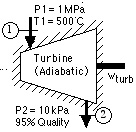
\includegraphics[width=0.3\textwidth]{steamTurb}
  \end{center}
  \begin{questionparts}
  \item Carefully plot the turbine process on the $h$-$s$ diagram and indicate the turbine work done on the plot.
  \item Using steam tables determine the specific work output of the turbine \answer{[1015 kJ/kg]}.
  \item Using steam tables determine the entropy generated by this process. \answer{[0.01 kJ/kg.K]}.
  \item Discuss these results and determine if this is a feasible turbine design.
  \end{questionparts}

  \question Adiabatic Evaluation of a R134a Compressor
  A young engineer was assigned to evaluate the compressor of a proposed R-134a refrigeration system shown below, and assumed it to be adiabatic.
  \begin{questionparts}
  \item Under this assumption, and ignoring kinetic and potential energy effects, determine the specific work input to the compressor \answer{[48.3 kJ/kg]}.
  \item His supervisor checked the results and told him that his assumption was incorrect and not physically feasible. On the $h$-$s$ diagram for R134a, draw the actual compression process (as assumed) as well as the equivalent isentropic compression process.
  \item Using the $h$-$s$ diagram, as well as relevant data evaluated at the inlet and outlet of the compressor, explain how she arrived at that conclusion.
  \end{questionparts}
  \newpage
  \question Previously, we provided a problem concerning a home refrigerator, and examining it's performance before and after adding an internal heat exchanger.
  \begin{center}
    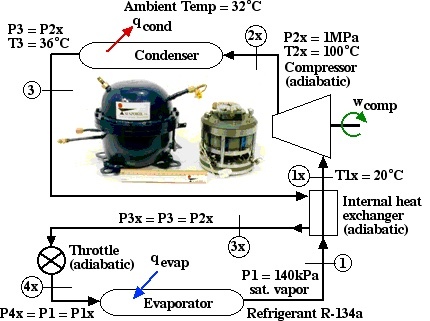
\includegraphics[width=0.5\textwidth]{ch4_HW_refrigHX}
  \end{center}
  \begin{questionparts}
  \item Plot the actual and the isentropic compressor processes on the enthalpy-entropy ($h$-$s$) diagram for both cases: with and without the internal heat exchanger.
  \item Using the R134a tables determine the actual compressor adiabatic efficiency ($\eta_C$) for both cases \answer{[75\%, 76\%]}
  \end{questionparts}

  \question A compressor is used to drive R134a through a heat pump.  R134a enters the compressor at a pressure $p_1$ = 400 kPa and a temperature $T_1$ = 40°C and leaves at a pressure $p_2$ = 1.6 MPa.  For the actual compressor, the exit tempearture is $T_2$ = 100°C.

  \begin{questionparts}
  \item Carefully plot the actual and isentropic compression processes on the $h$-$s$ diagram and indicate the actual and isentropic specific work done to drive the compressor on the plot.
  \item Using R134a refrigerant tables, determine the specific work required to drive the compressor \answer{[43.5 kJ/kg]}.
  \item Using R134a refrigerant tables, determine the adiabatic efficiency of the compressor \answer{[$\eta_C$ = 78\%]}.
  \item Discuss these results and determine if this is a feasible compressor design.
  \end{questionparts}
  \newpage
  \question In Example \ref{ex:T700} we did an ideal thermodynamic analysis of the General Electric T700 helicopter gas turbine engine, shown in the following schematic diagram:
  \begin{center}
    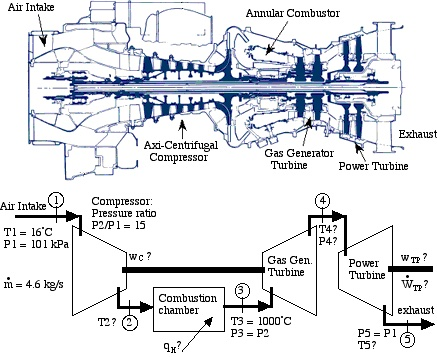
\includegraphics[width=.8\linewidth]{gas_turbine}
  \end{center}

  Notice again that there are two turbines operating on independent output shafts. The High Pressure (first) turbine, named the Gas Generator turbine, is directly connected by a shaft to the compressor. Its sole purpose is to drive the the compressor, thus the energy output of this turbine must equal the energy consumed by the compressor. The Low Pressure (second) turbine, named the Power turbine, is connected via gearing to the helicopter rotor.

  In Example \ref{ex:T700} we assumed that the compressor and both turbines were isentropic. In this exercise we wish to extend the analysis to non-isentropic compressor and turbines.

  Assume that the compressor adiabatic efficiency $\eta_C$ = 88\%, and that each turbine has an adiabatic efficiency $\eta_T$ = 86\%.

  \begin{questionparts}
  \item Sketch the entire process on an $h$-$s$ diagram, clearly showing the 5 stations on the diagram and the relevant isentropic and constant pressure lines. Indicate the relevant actual and isentropic work values on the sketch.
  \item Determine the actual energy consumed by the compressor \answer{[$w_{C,act}$ = 373 kJ/kg]}, and the actual temperature at the outlet of the compressor \answer{[$T_{2a}$ = 628K]}.
  \item Determine the heat energy absorbed by the working gas in the combustion chamber \answer{[$q_H$ = 709 kJ/kg]}.
  \item Determine the actual temperature [$T_{4a}$ = 934K] and the pressure [$P_4$ = 366 kPa] at the outlet of the gas generator turbine.
  \item Determine the actual temperature [$T_{5a}$] and energy output of the power turbine [$w_{PT,act}$ = 252 kJ/kg].
  \item Given that the mass flow rate of the working gas through the system is 4.6 kg/s, determine the actual power output of the power turbine \answer{[1161 kW]}.
  \item Determine the thermal efficiency ($\eta_{th}$) of the T700 gas turbine. Compare this value to the equivalent reversible thermal efficiency and discuss your results.
  \end{questionparts}

\end{homework}


